\chapter{}
\label{append}

\section{Statistical Tests}
\begin{figure}[!htb]
	\centering
	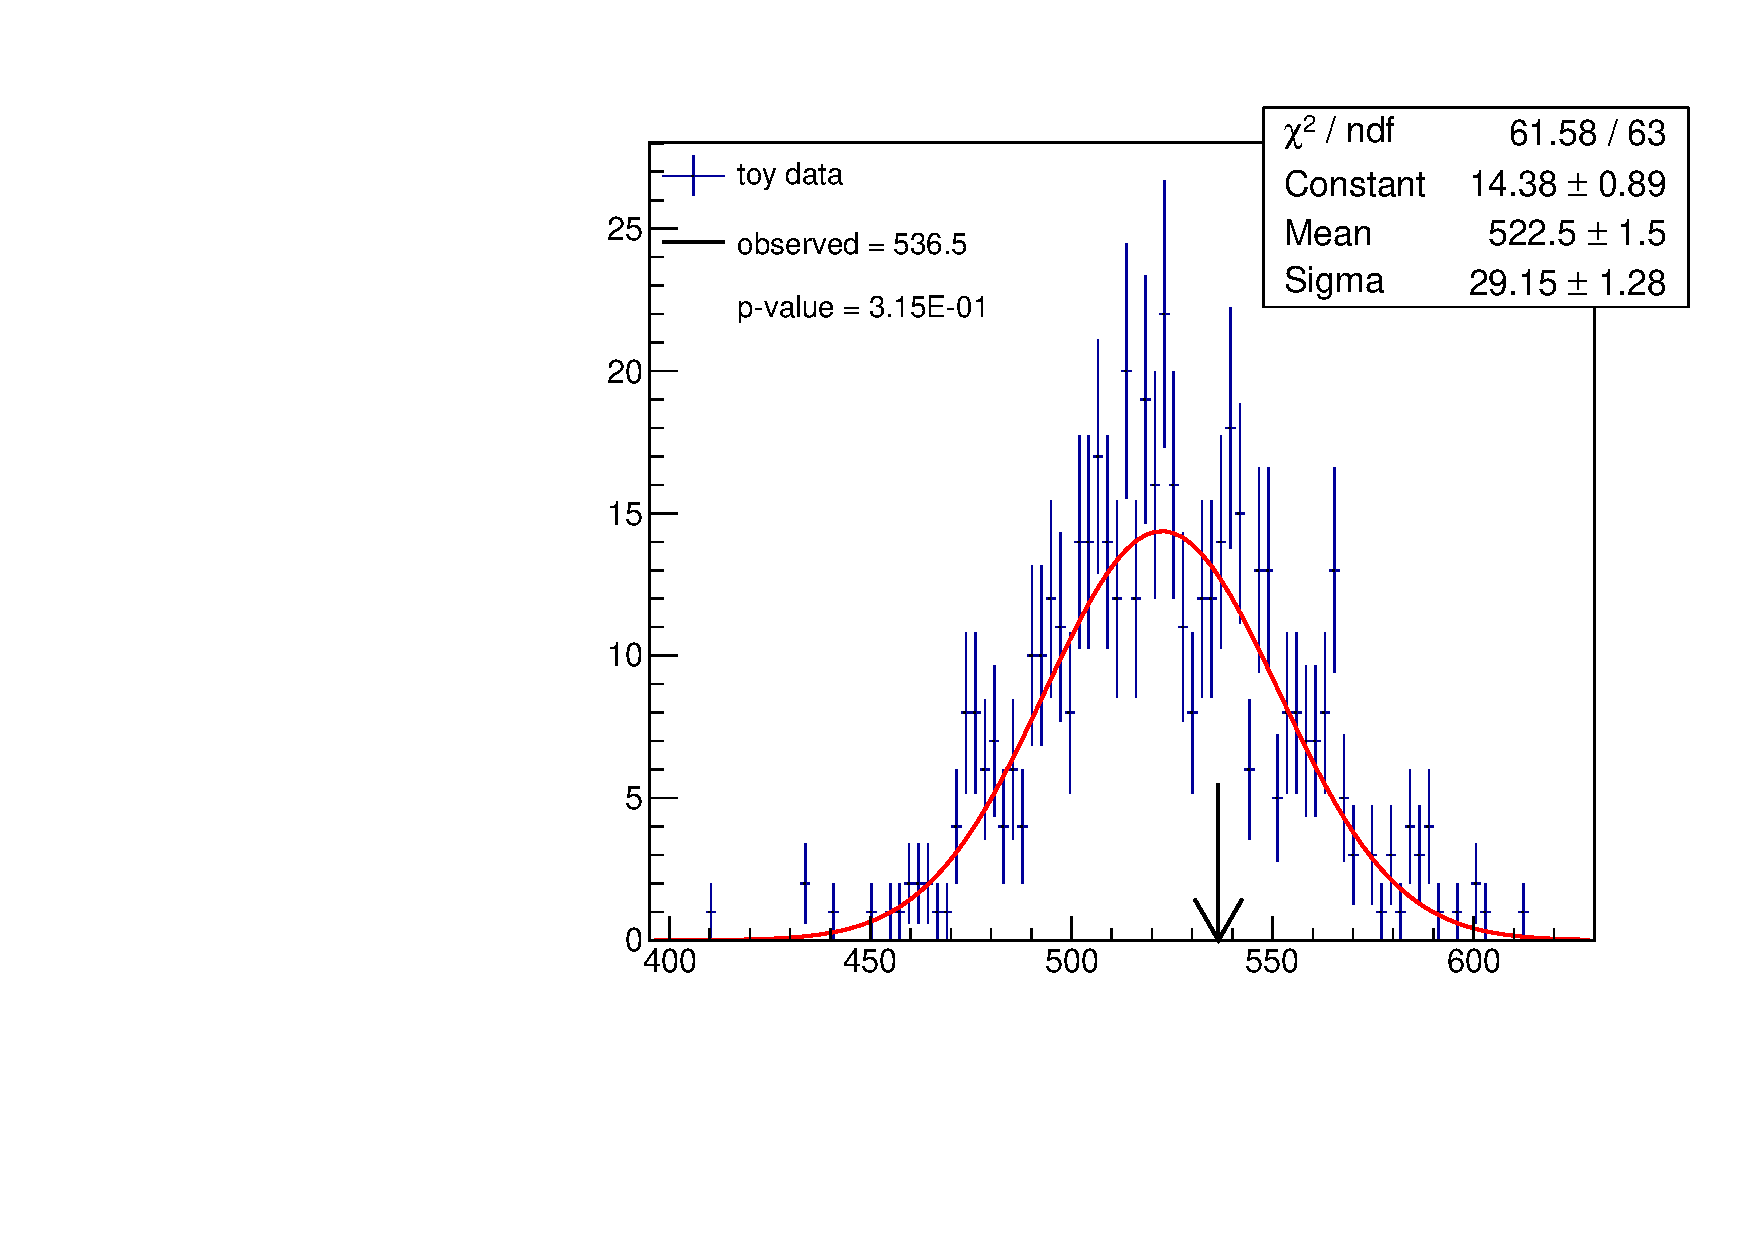
\includegraphics[width=0.75\textwidth]{Figures/gof_plot.pdf}
	\caption{Full Run 2 Goodness of Fit test plot with 500 toys.}
	\label{fig:gofplot}
\end{figure}

\begin{figure}[!htb]
	\centering
	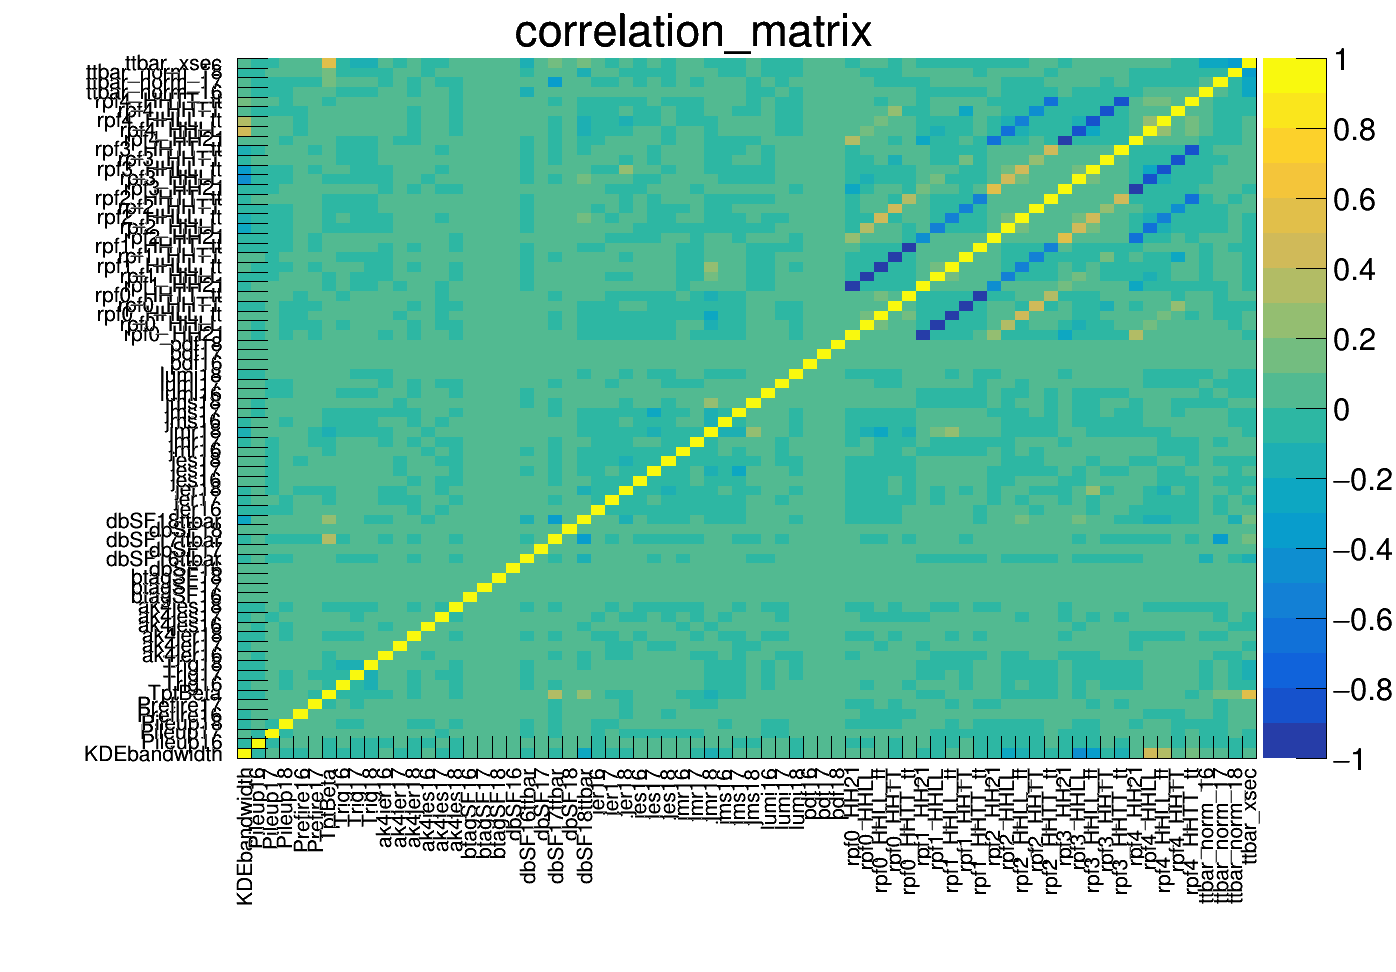
\includegraphics[width=0.75\textwidth]{Figures/correlation_matrix.png}
	\caption{Full Run 2 Correlation Matrix.}
	\label{fig:corrMatrixplot}
\end{figure}


\begin{figure}[!htb]
	\centering
	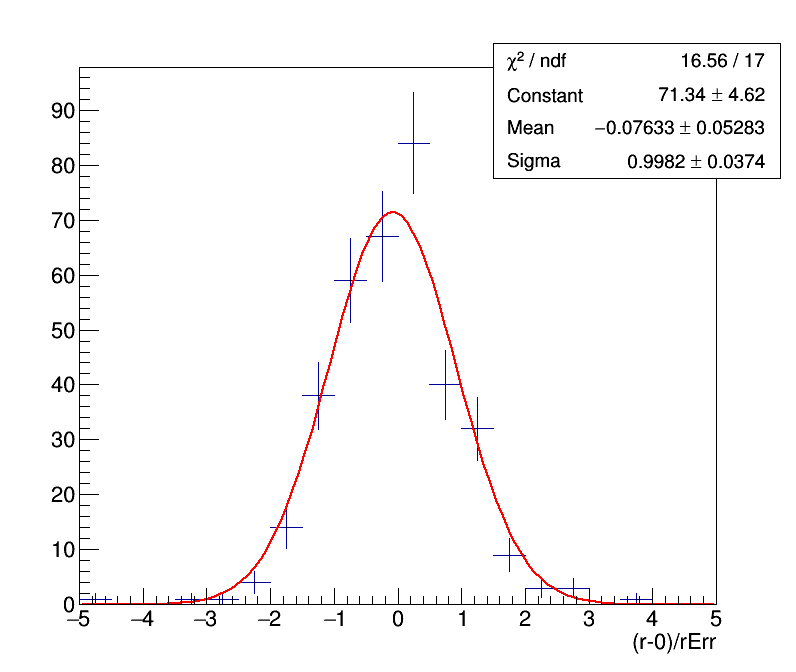
\includegraphics[width=0.4\textwidth]{Figures/signalInjection0_500_sigpull_1000.png}
	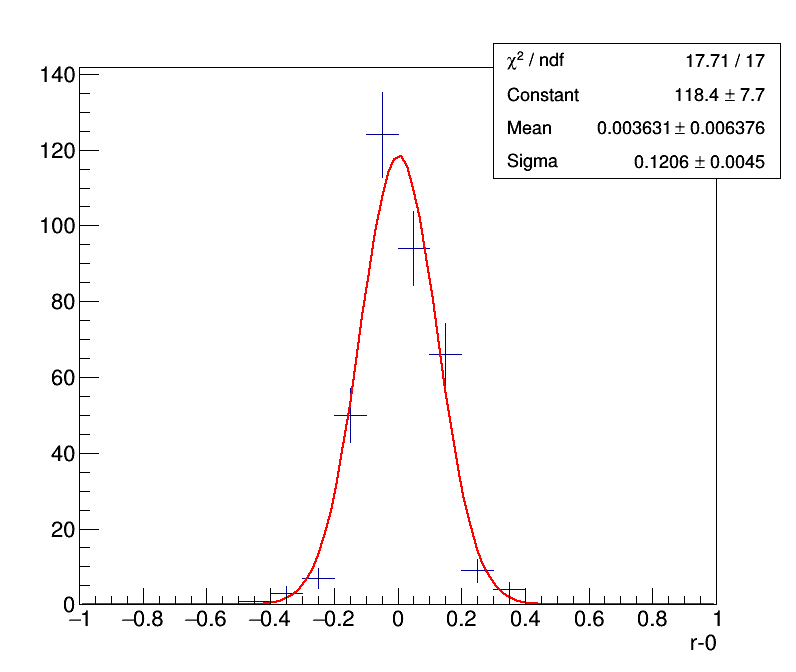
\includegraphics[width=0.4\textwidth]{Figures/signalInjection0_500_sigstrength_1000.png}
	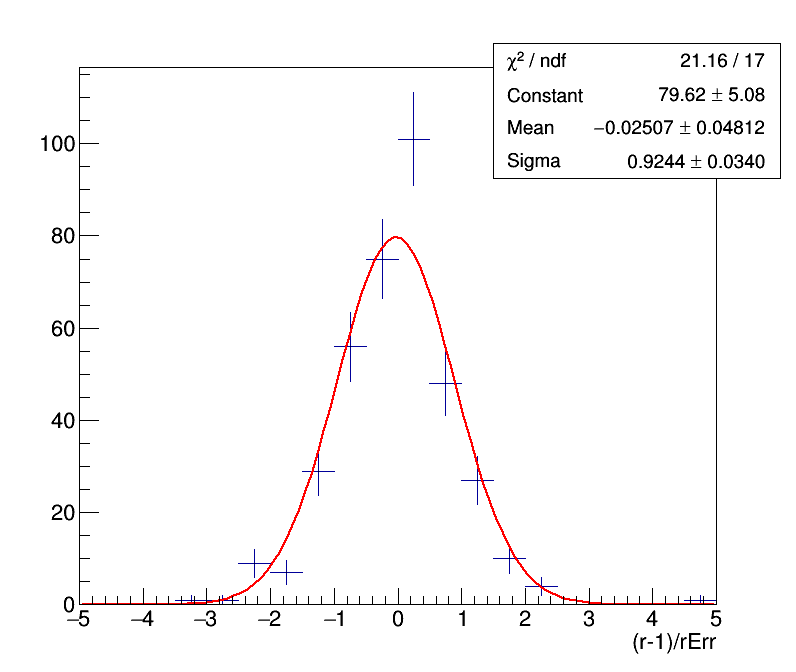
\includegraphics[width=0.4\textwidth]{Figures/signalInjection1_500_sigpull_1000.png}
	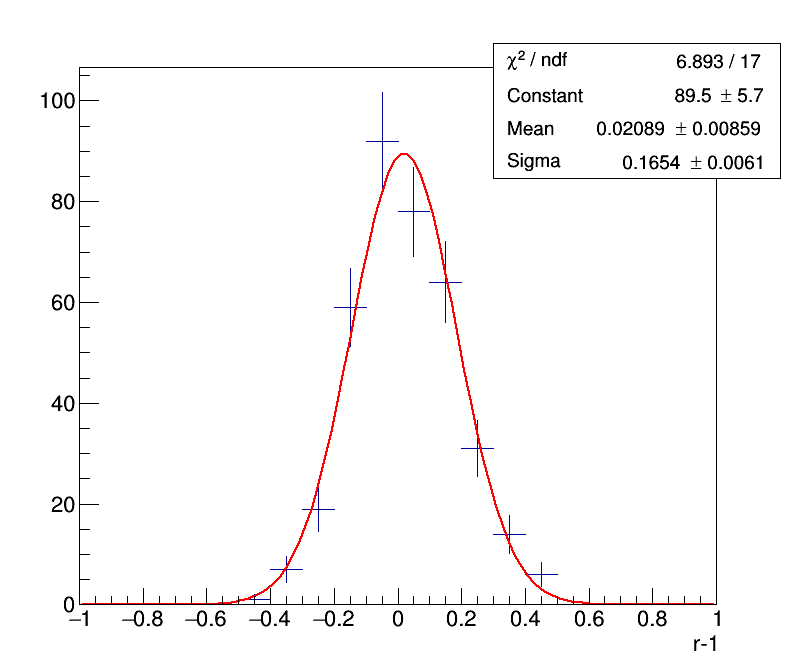
\includegraphics[width=0.4\textwidth]{Figures/signalInjection1_500_sigstrength_1000.png}
	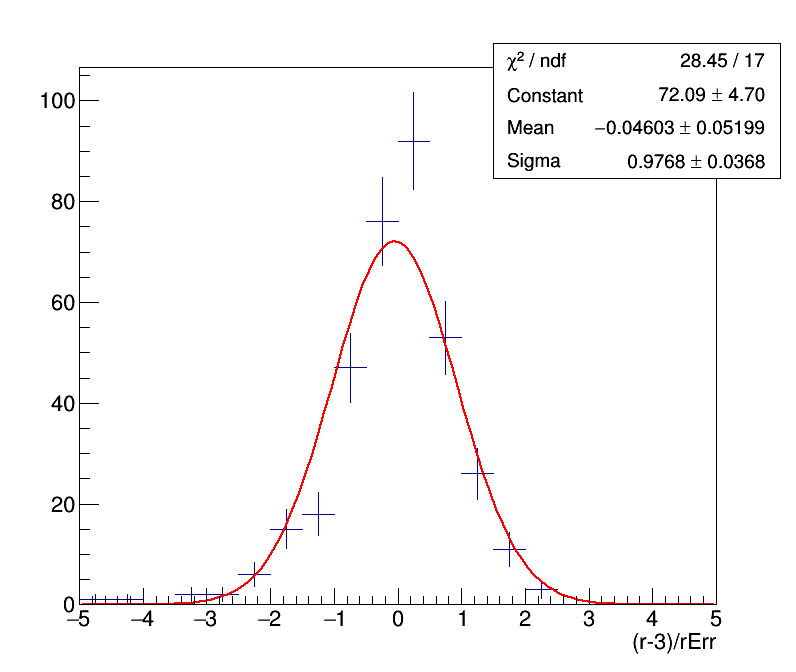
\includegraphics[width=0.4\textwidth]{Figures/signalInjection3_500_sigpull_1000.png}
	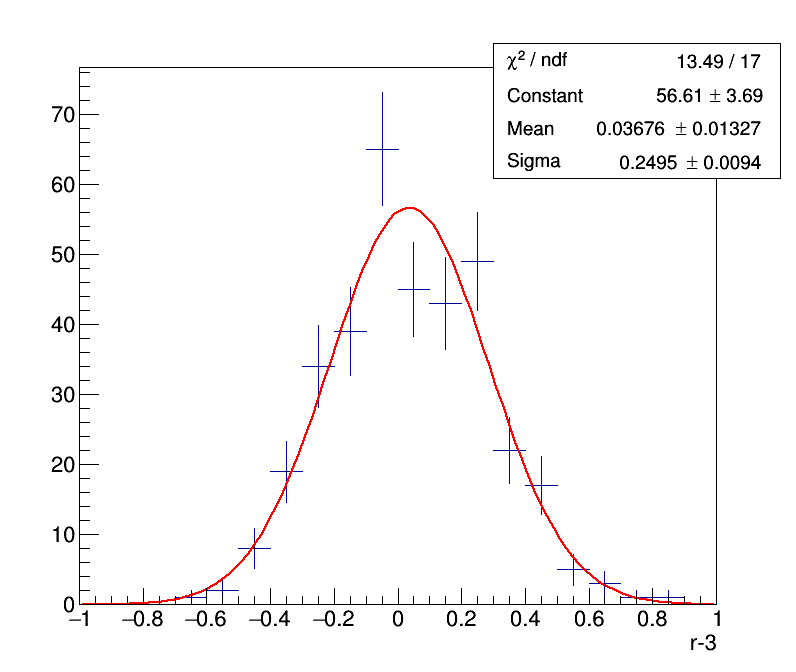
\includegraphics[width=0.4\textwidth]{Figures/signalInjection3_500_sigstrength_1000.png}
	\caption{Signal Injection (Left Column is Pull and Right is Strength) for Full Run 2 at 1 TeV for r = 0, 1, 3 with 500 toys.}
	\label{fig:signalInjection1000plot}
\end{figure}

\begin{figure}[!htb]
	\centering
	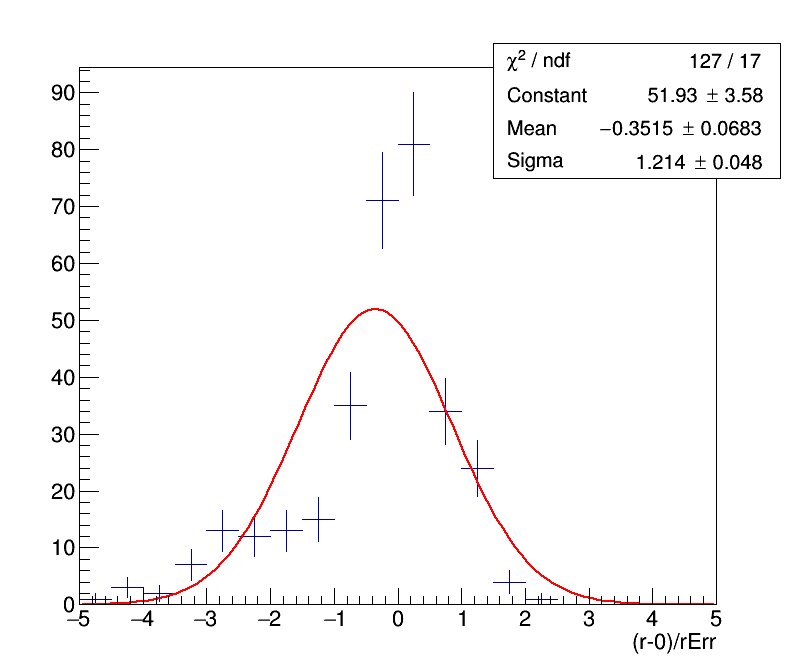
\includegraphics[width=0.4\textwidth]{Figures/signalInjection0_500_sigpull_2000.png}
	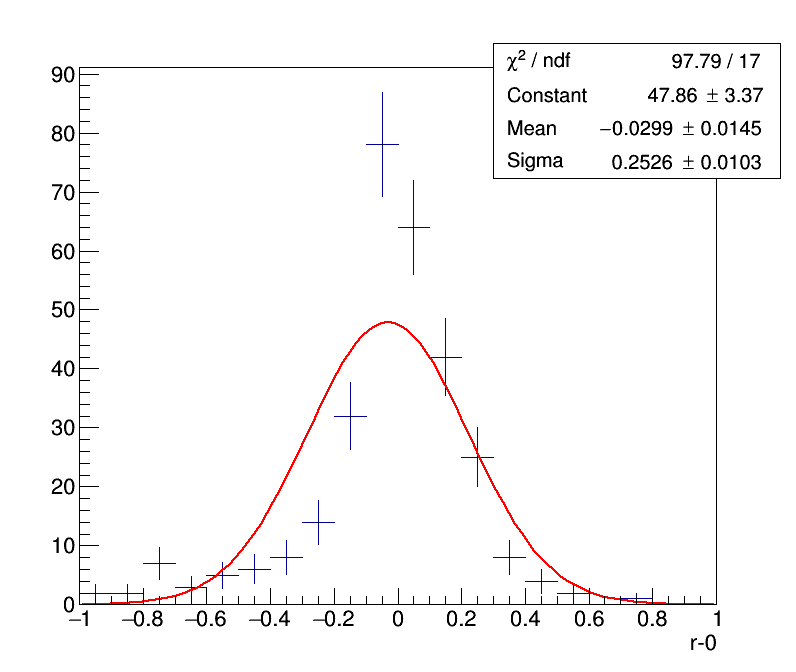
\includegraphics[width=0.4\textwidth]{Figures/signalInjection0_500_sigstrength_2000.png}
	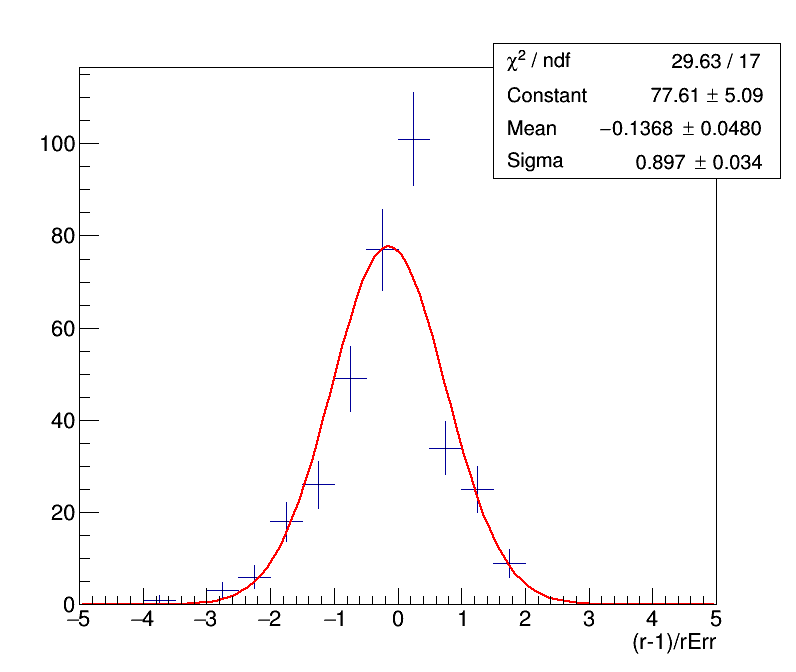
\includegraphics[width=0.4\textwidth]{Figures/signalInjection1_500_sigpull_2000.png}
	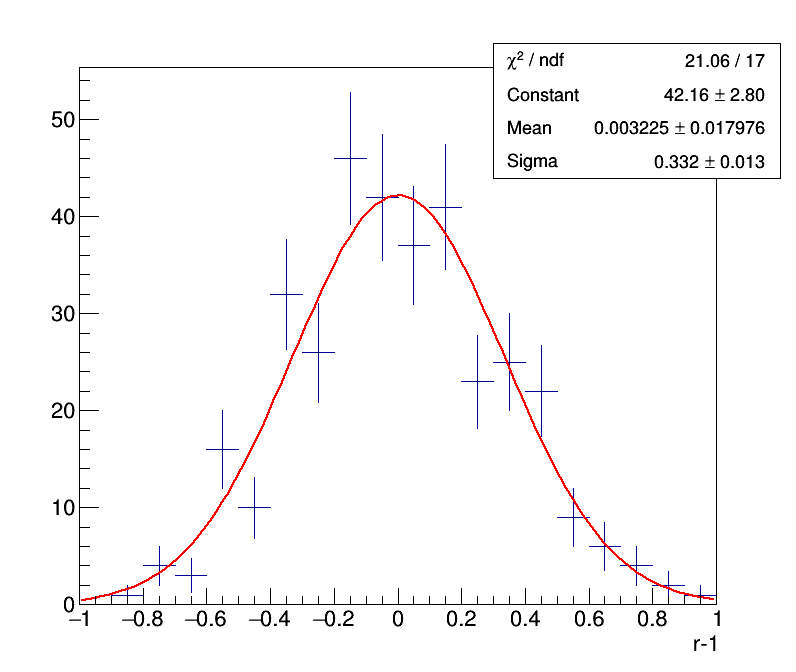
\includegraphics[width=0.4\textwidth]{Figures/signalInjection1_500_sigstrength_2000.png}
	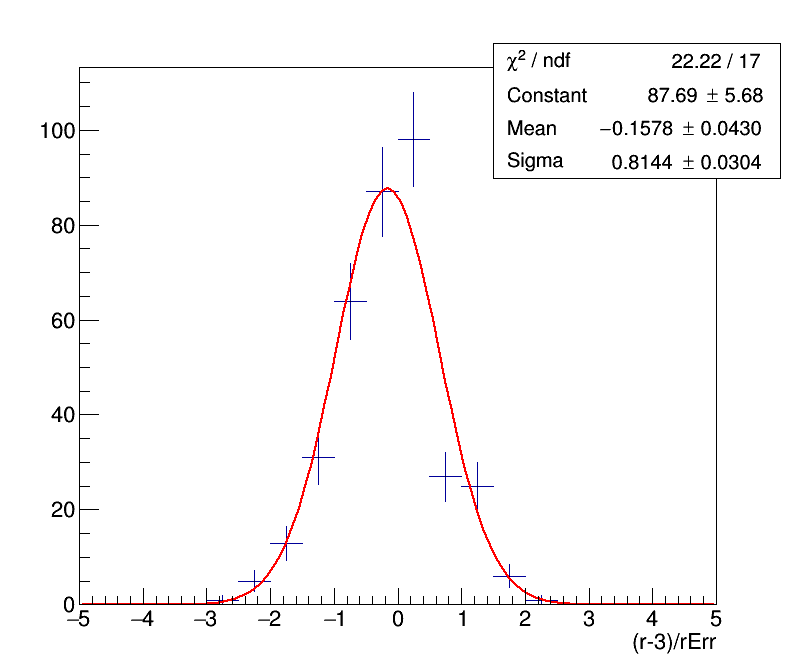
\includegraphics[width=0.4\textwidth]{Figures/signalInjection3_500_sigpull_2000.png}
	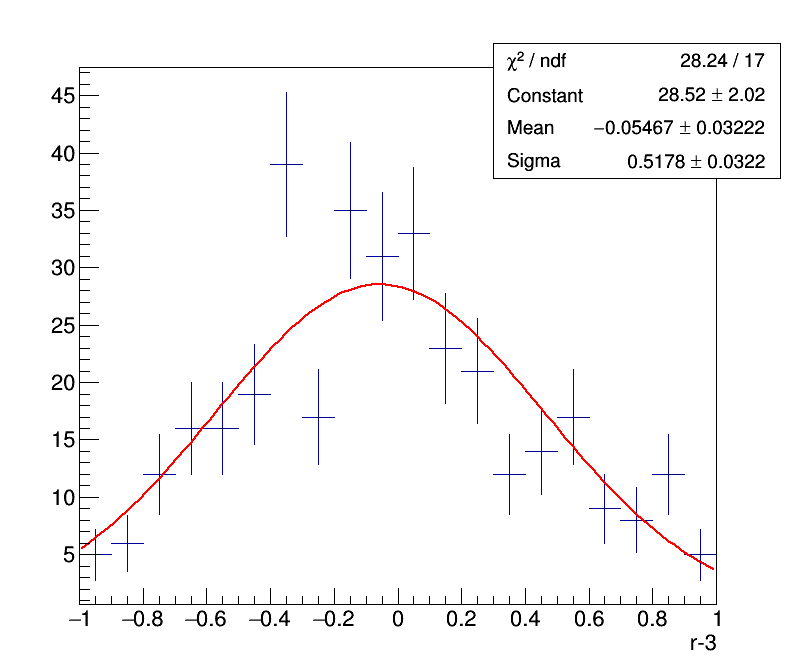
\includegraphics[width=0.4\textwidth]{Figures/signalInjection3_500_sigstrength_2000.png}
	\caption{Signal Injection (Left Column is Pull and Right is Strength) for Full Run 2 at 2 TeV for r = 0, 1, 3 with 500 toys.}
	\label{fig:signalInjection2000plot}
\end{figure}

\begin{figure}[!htb]
	\centering
	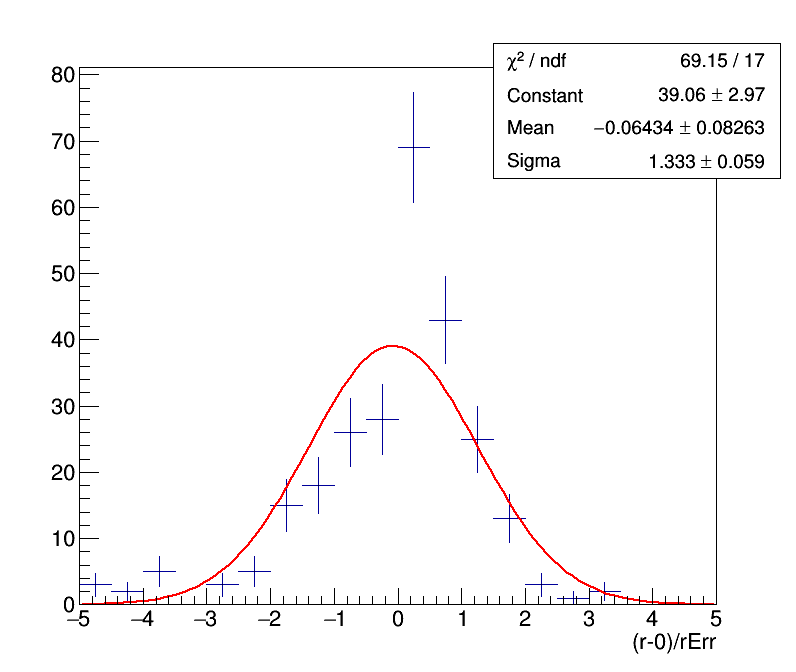
\includegraphics[width=0.4\textwidth]{Figures/signalInjection0_500_sigpull_3000.png}
	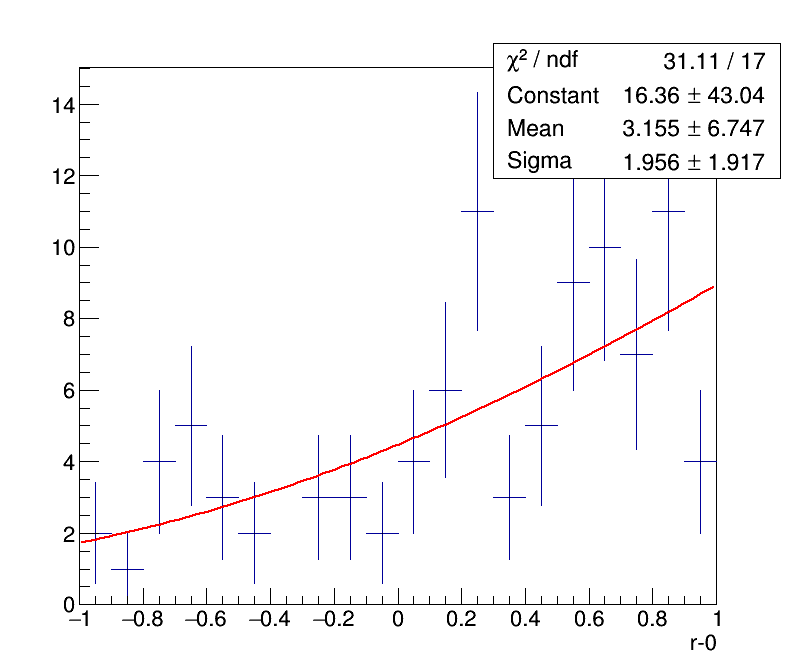
\includegraphics[width=0.4\textwidth]{Figures/signalInjection0_500_sigstrength_3000.png}
	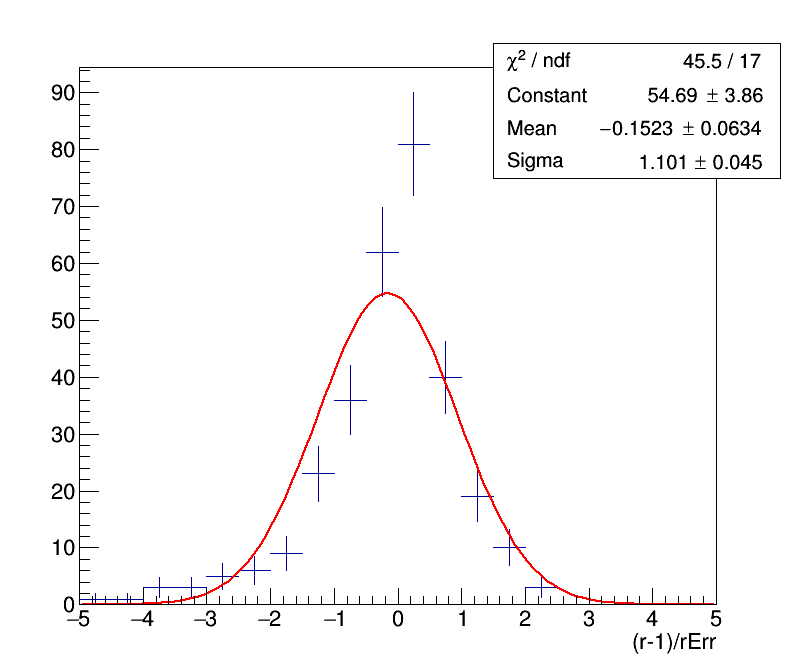
\includegraphics[width=0.4\textwidth]{Figures/signalInjection1_500_sigpull_3000.png}
	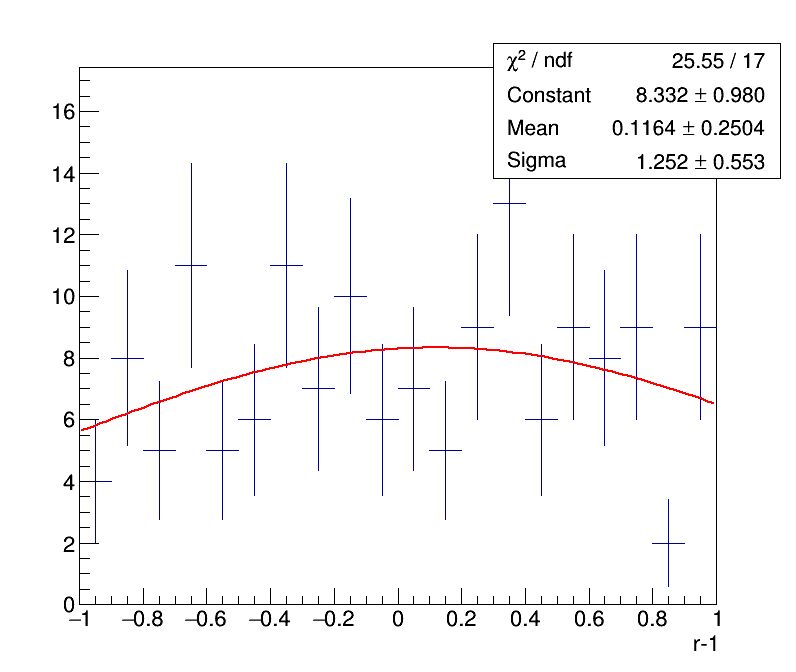
\includegraphics[width=0.4\textwidth]{Figures/signalInjection1_500_sigstrength_3000.png}
	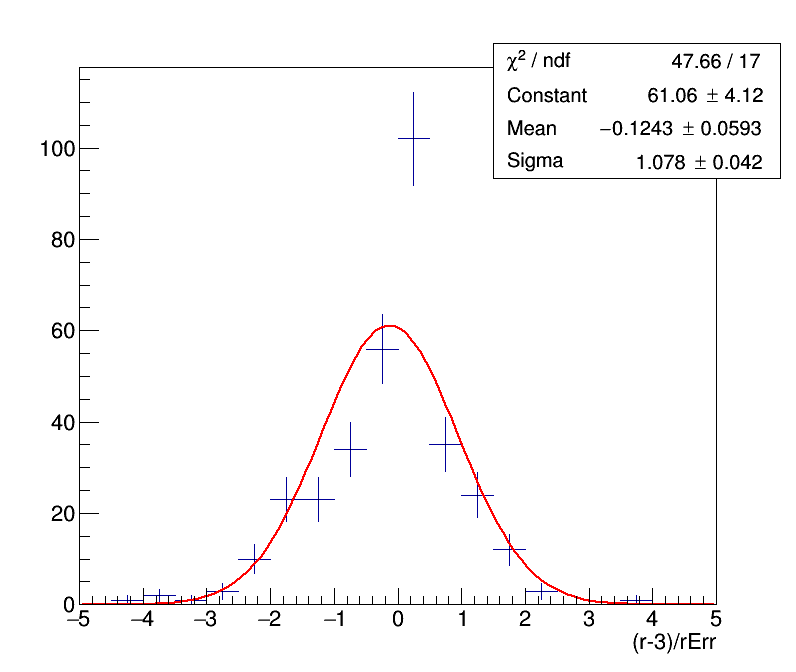
\includegraphics[width=0.4\textwidth]{Figures/signalInjection3_500_sigpull_3000.png}
	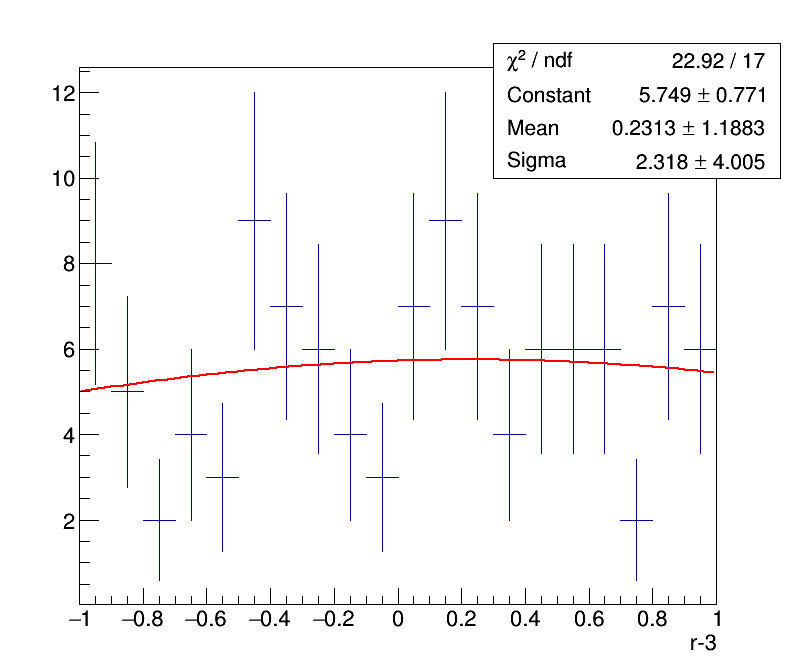
\includegraphics[width=0.4\textwidth]{Figures/signalInjection3_500_sigstrength_3000.png}
	\caption{Signal Injection (Left Column is Pull and Right is Strength) for Full Run 2 at 3 TeV for r = 0, 1, 3 with 500 toys.}
	\label{fig:signalInjection3000plot}
\end{figure}
It is obvious that there may be some bias at the 2 and 3 TeV points when we inject $r = 0$. However, this is actually due to there being poor statistics at those mass points. When we simulate a higher integrated luminosity we get a plot with a more reasonable shape.
\begin{figure}[!htb]
	\centering
	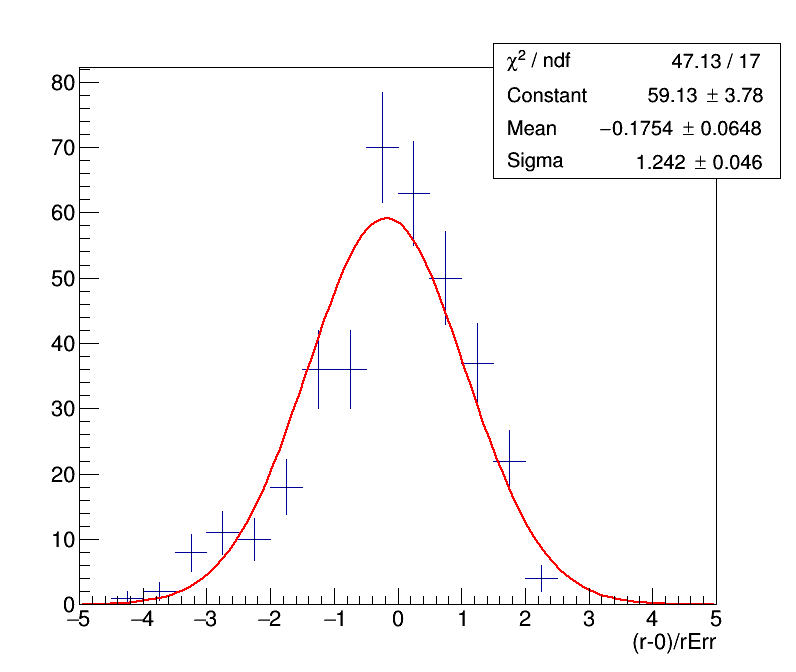
\includegraphics[width=0.5\textwidth]{Figures/signalInjection0_500_sigpull_2000_HIGHYIELD.png}
	\caption{Signal Injection for Full Run 2 at 2 TeV for r = 0 with 500 toys and a simulated higher integrated luminosity.}
	\label{fig:signalInjection2000plotHIGH}
\end{figure}
\clearpage
\subsection{F-Test}
We performed an F-test to optimize the function used to perform the fit. The results show that a 2nd order in $\mjred$ and 2nd order in $\mred$ fit function is most optimal. 
\begin{figure}[!htb]
	\centering
	% 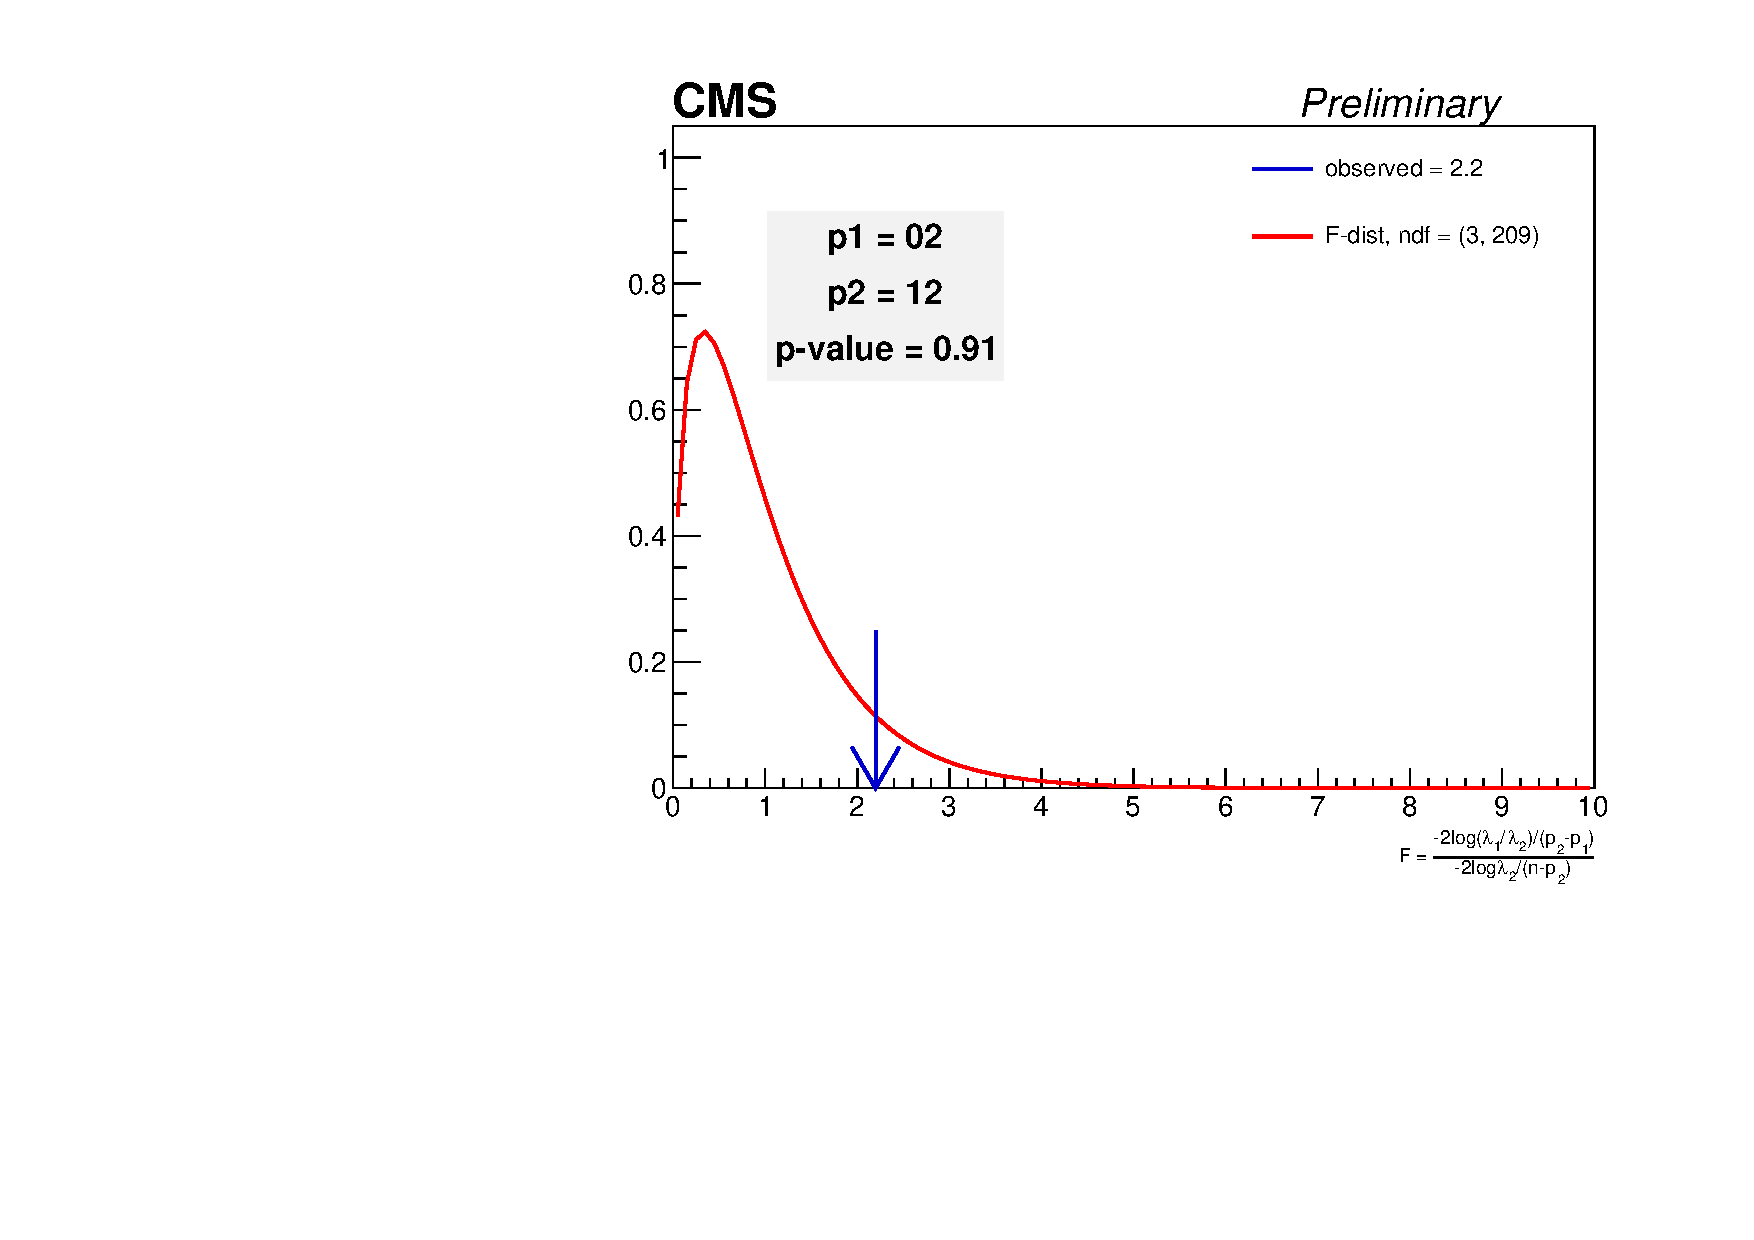
\includegraphics[width=0.4\textwidth]{Figures/ftest_vs_FTESTpol02_pol12_notoys.pdf}
	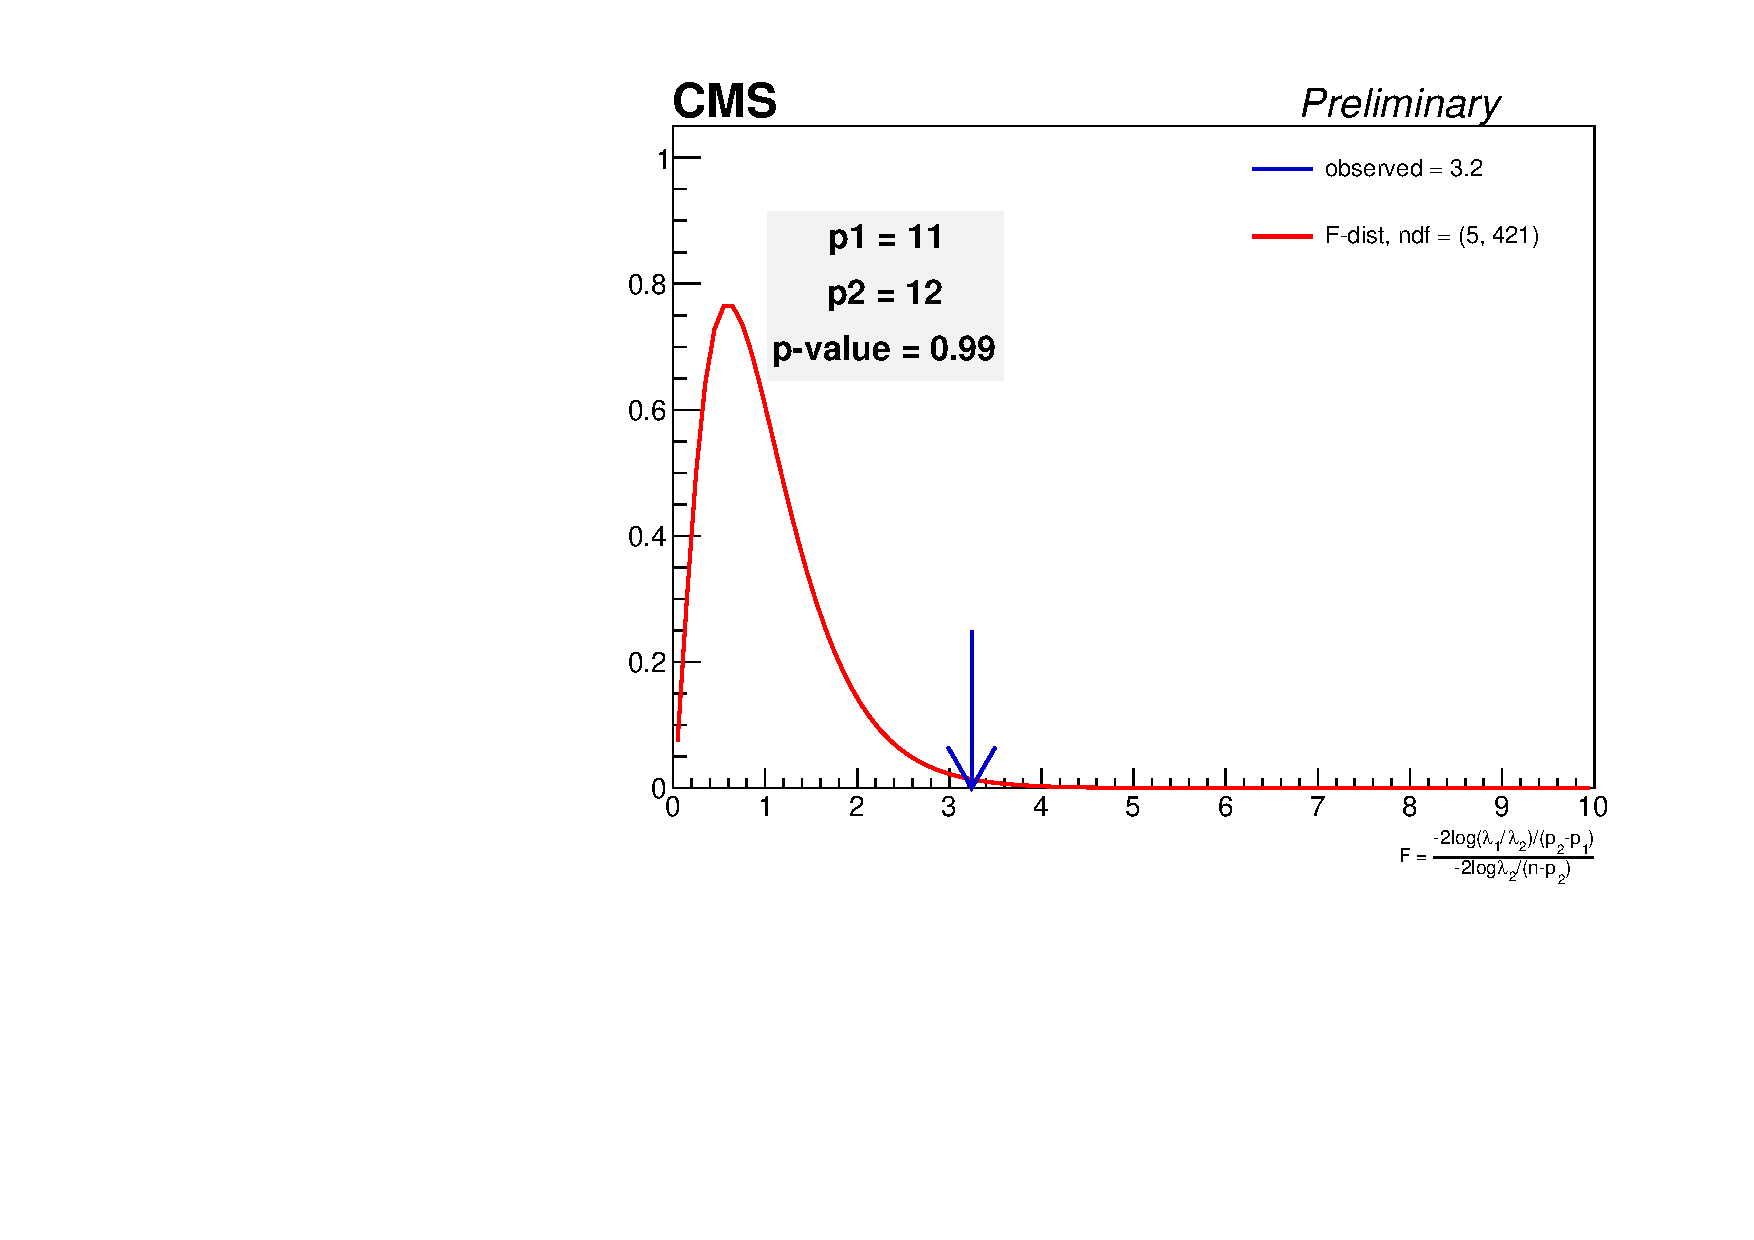
\includegraphics[width=0.4\textwidth]{Figures/ftest_vs_FTESTBNEWpol11_pol12_notoys.pdf}
	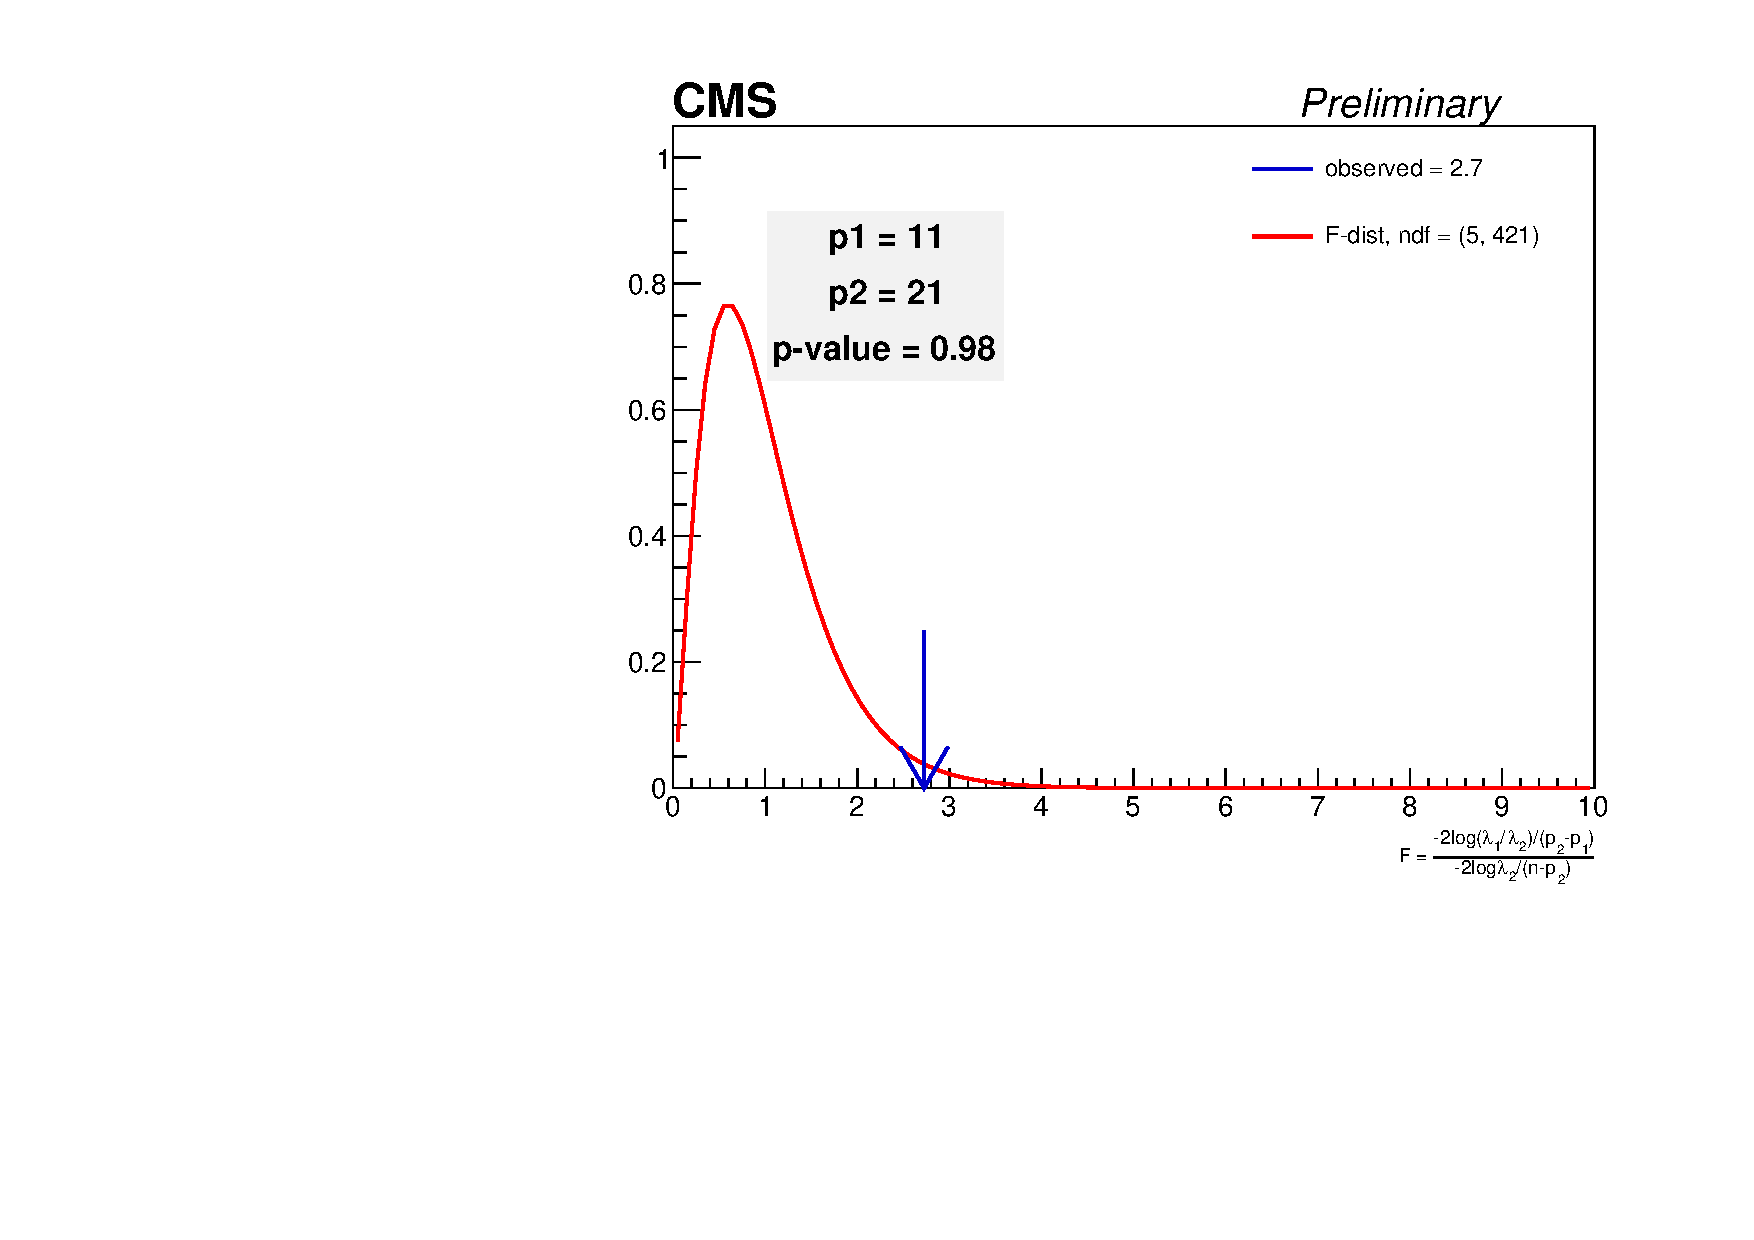
\includegraphics[width=0.4\textwidth]{Figures/ftest_vs_FTESTBNEWpol11_pol21_notoys.pdf}
	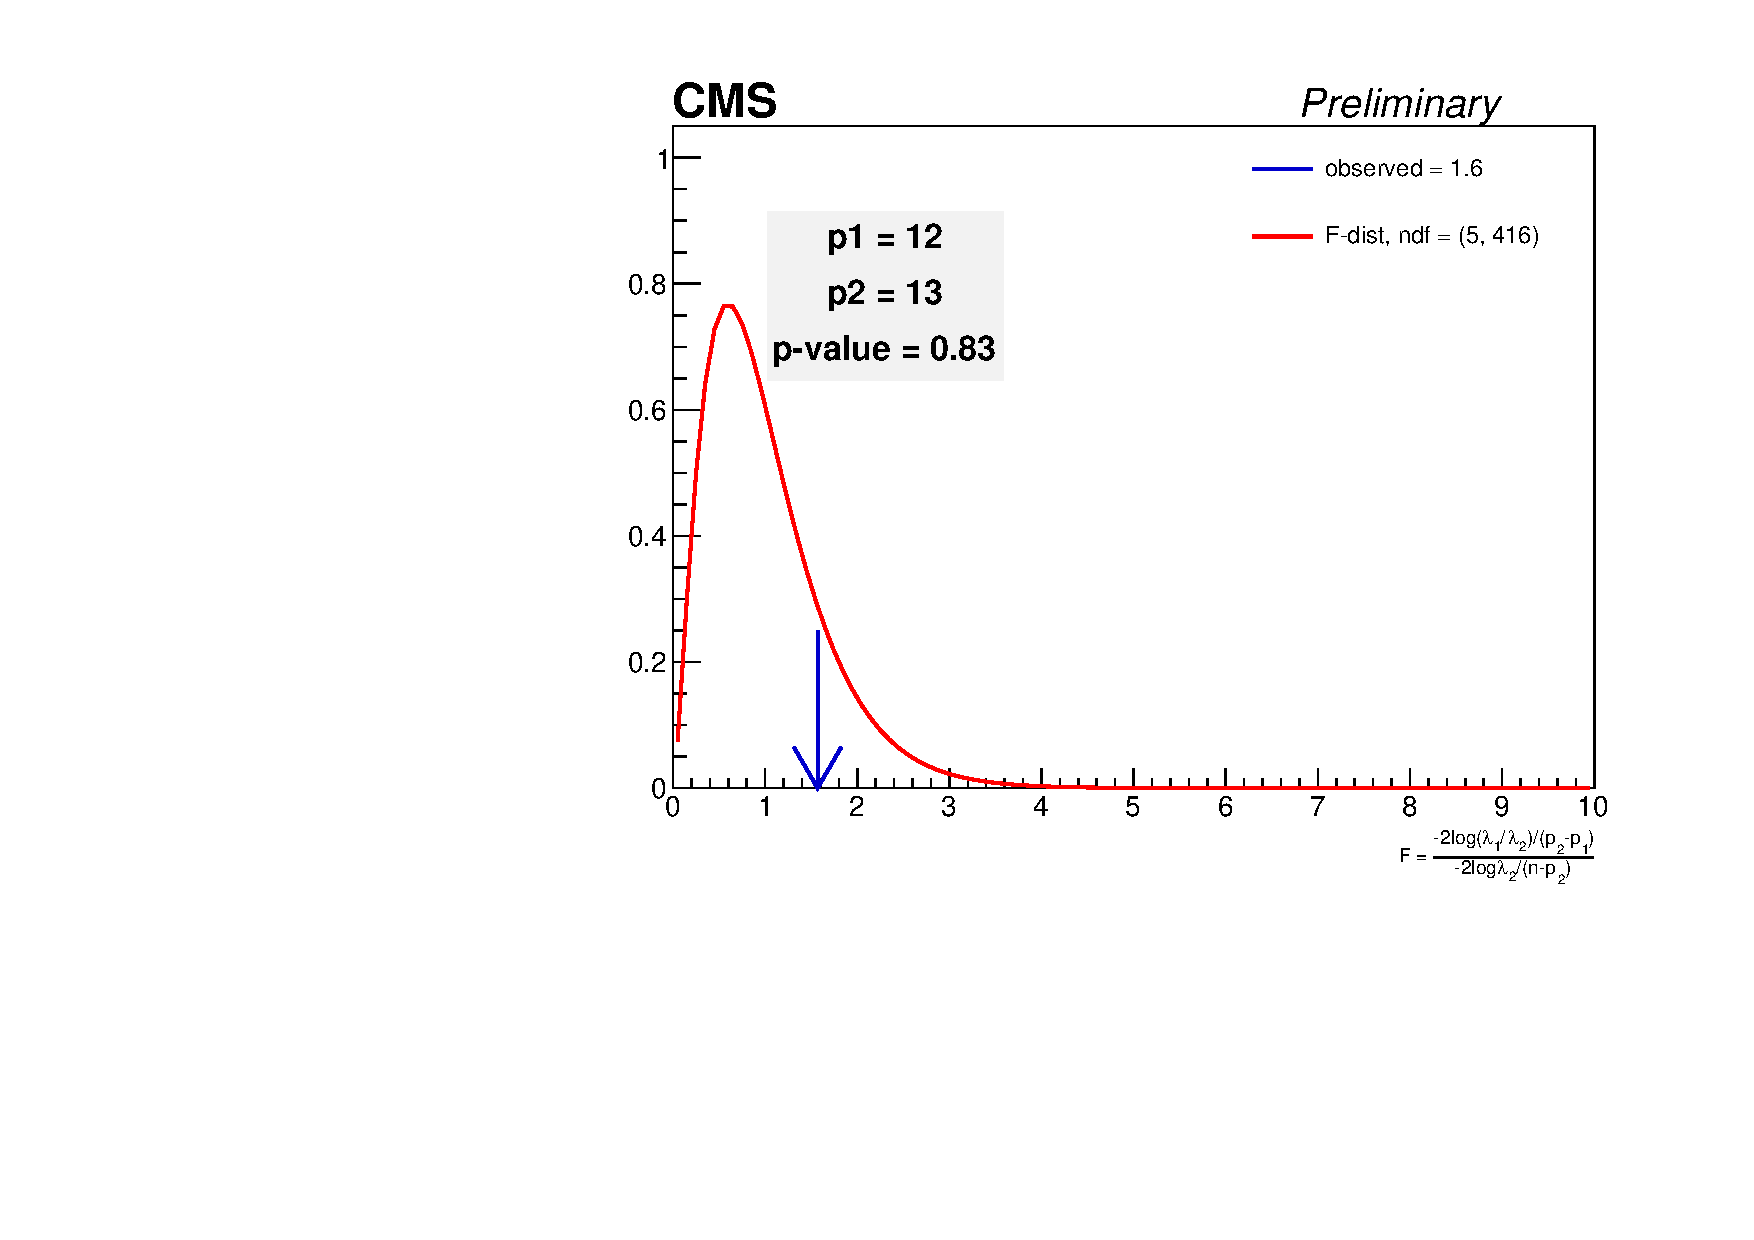
\includegraphics[width=0.4\textwidth]{Figures/ftest_vs_FTESTBNEWpol12_pol13_notoys.pdf}
	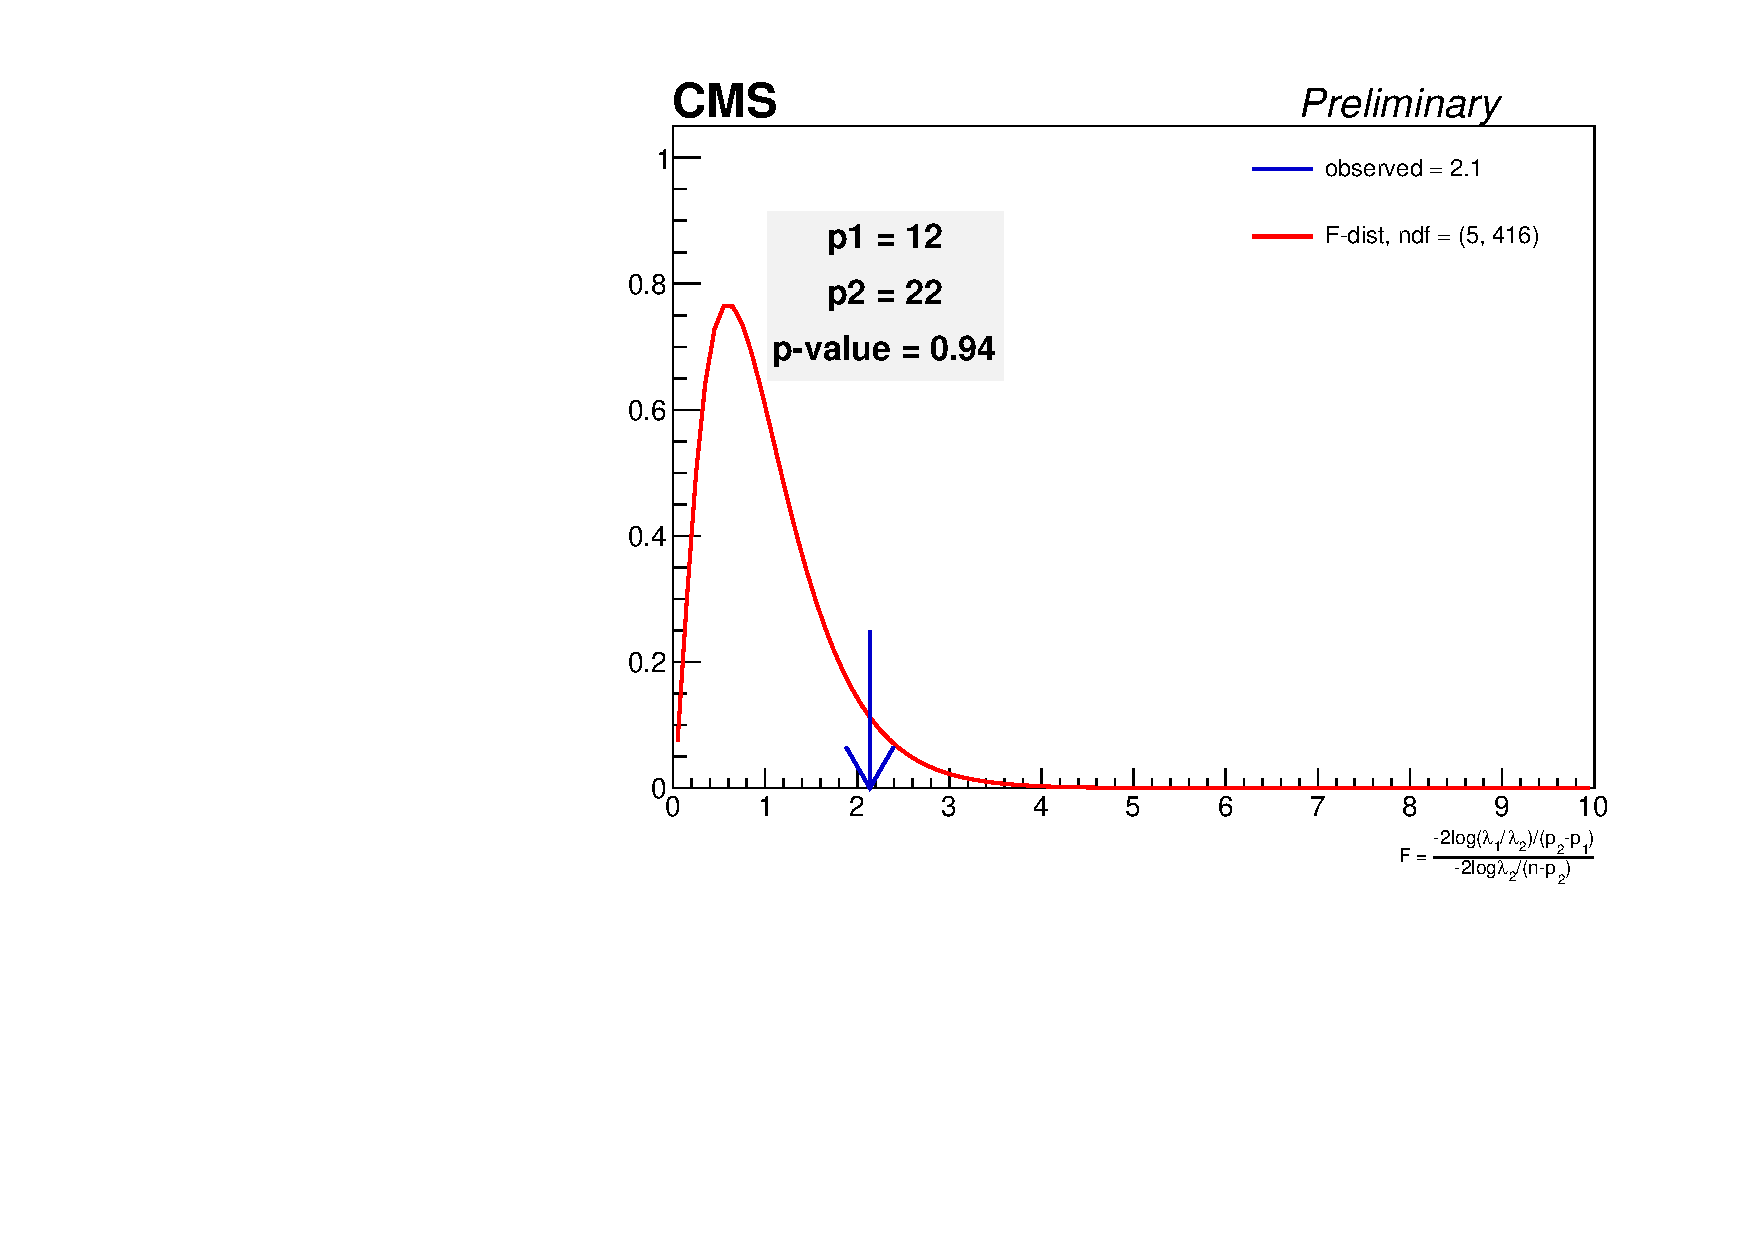
\includegraphics[width=0.4\textwidth]{Figures/ftest_vs_FTESTBNEWpol12_pol22_notoys.pdf}
	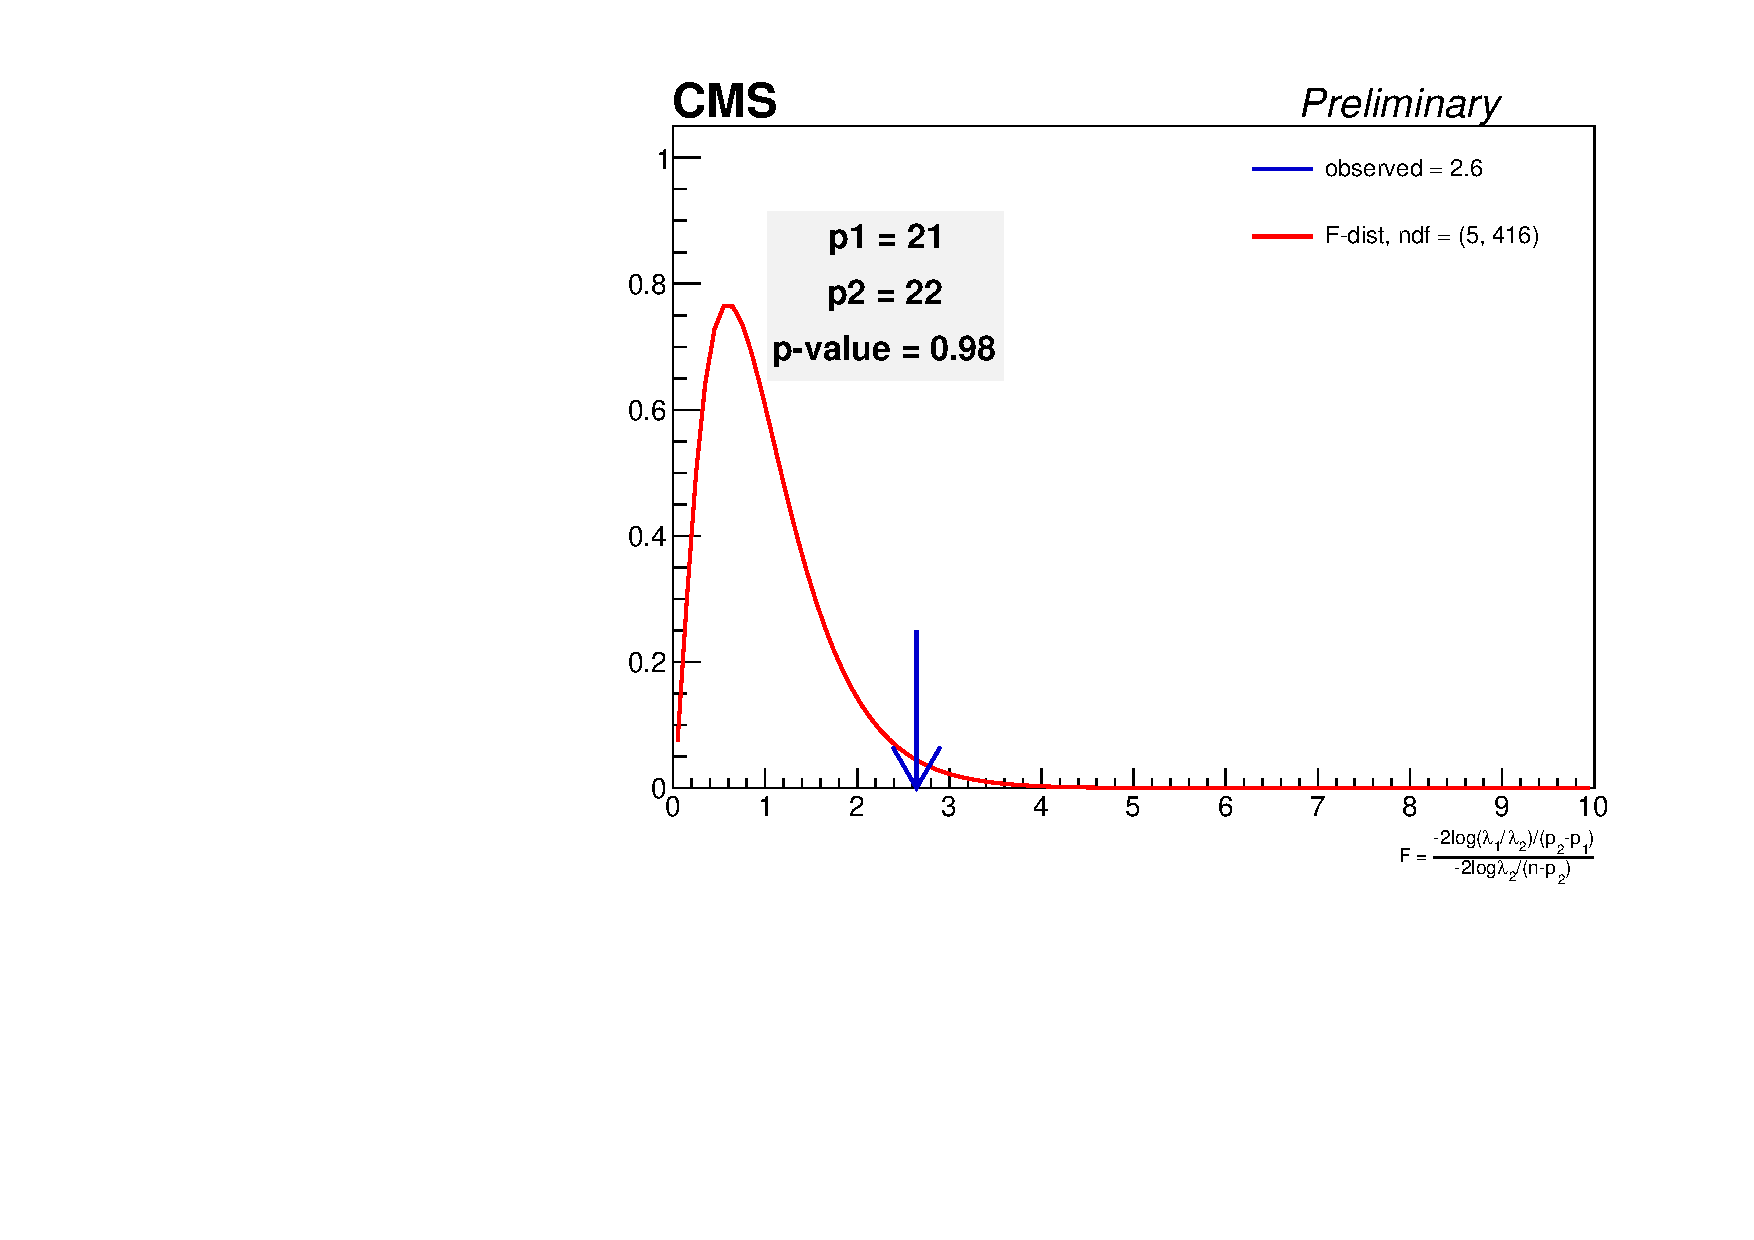
\includegraphics[width=0.4\textwidth]{Figures/ftest_vs_FTESTBNEWpol21_pol22_notoys.pdf}
	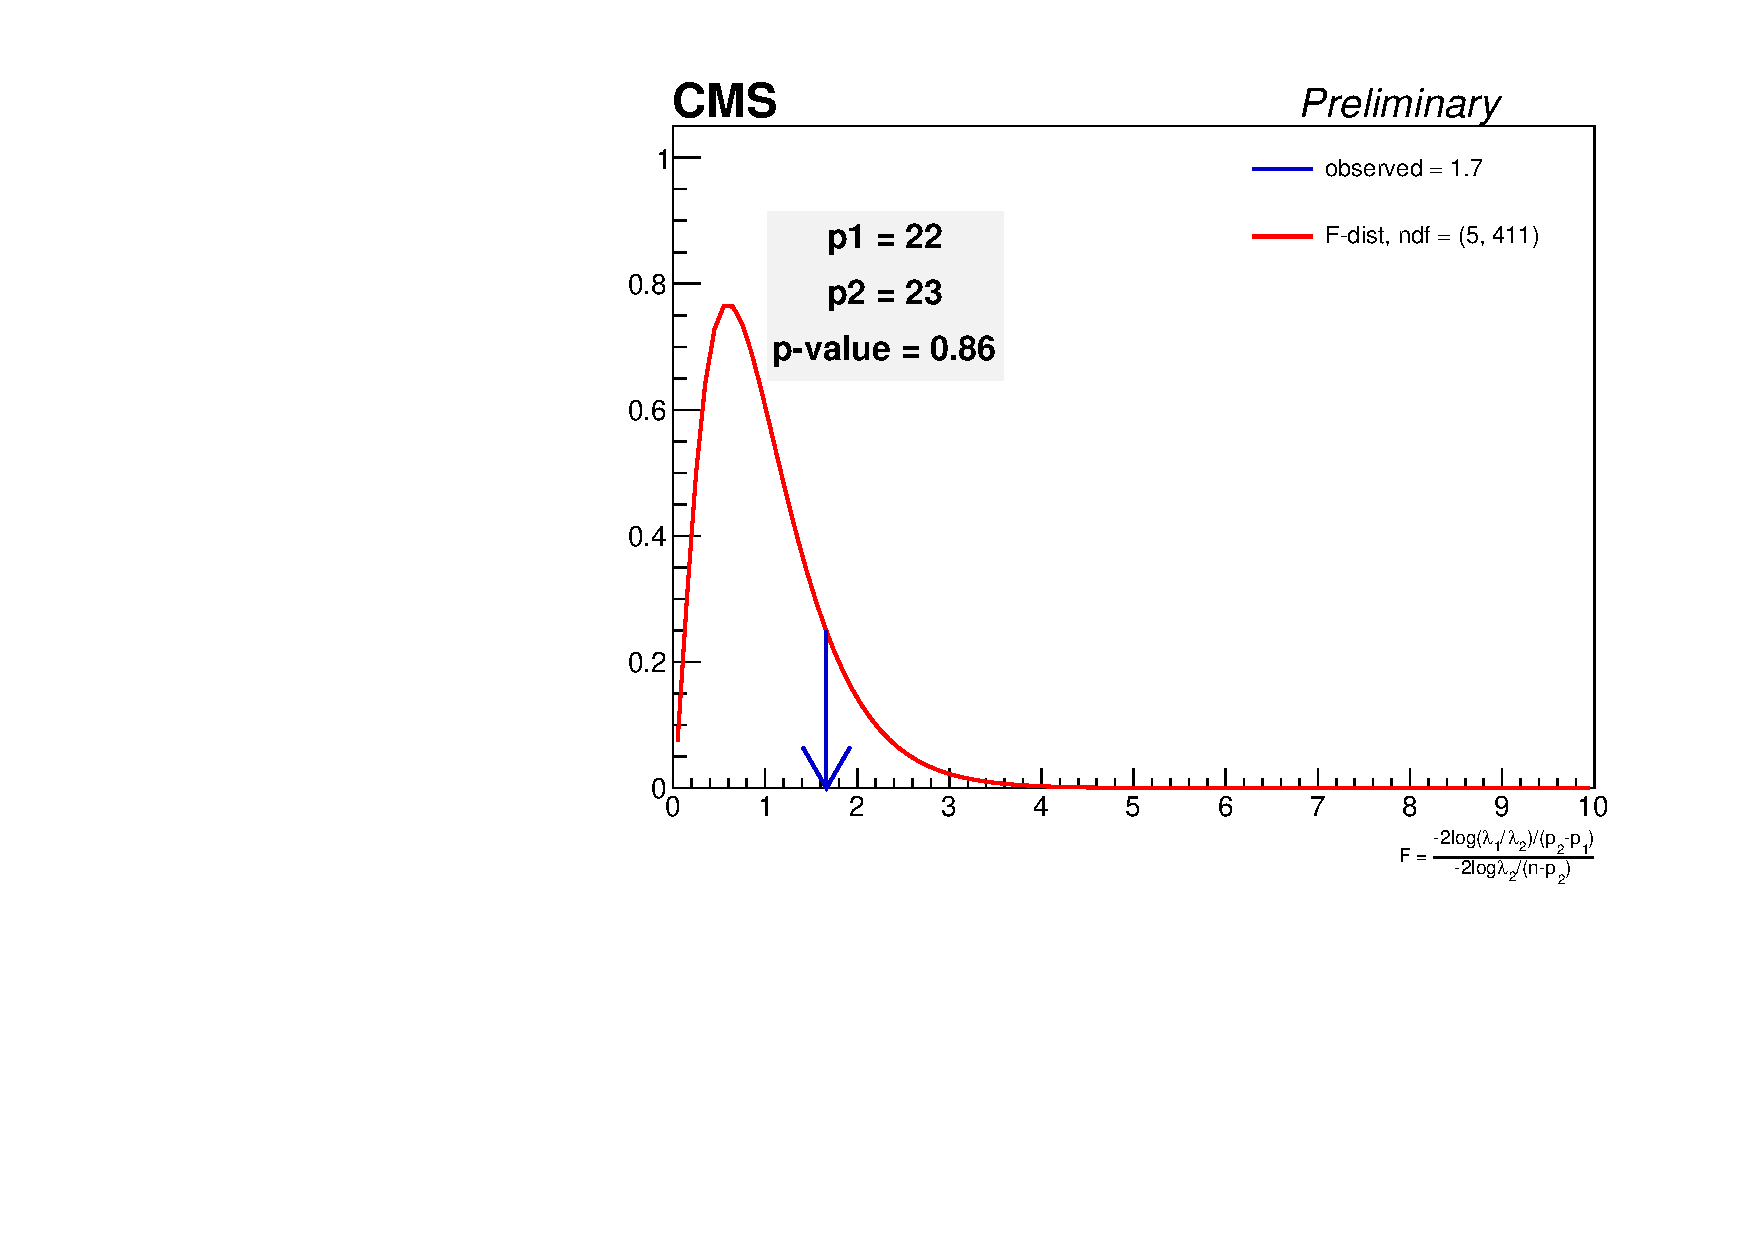
\includegraphics[width=0.4\textwidth]{Figures/ftest_vs_FTESTBNEWpol22_pol23_notoys.pdf}
	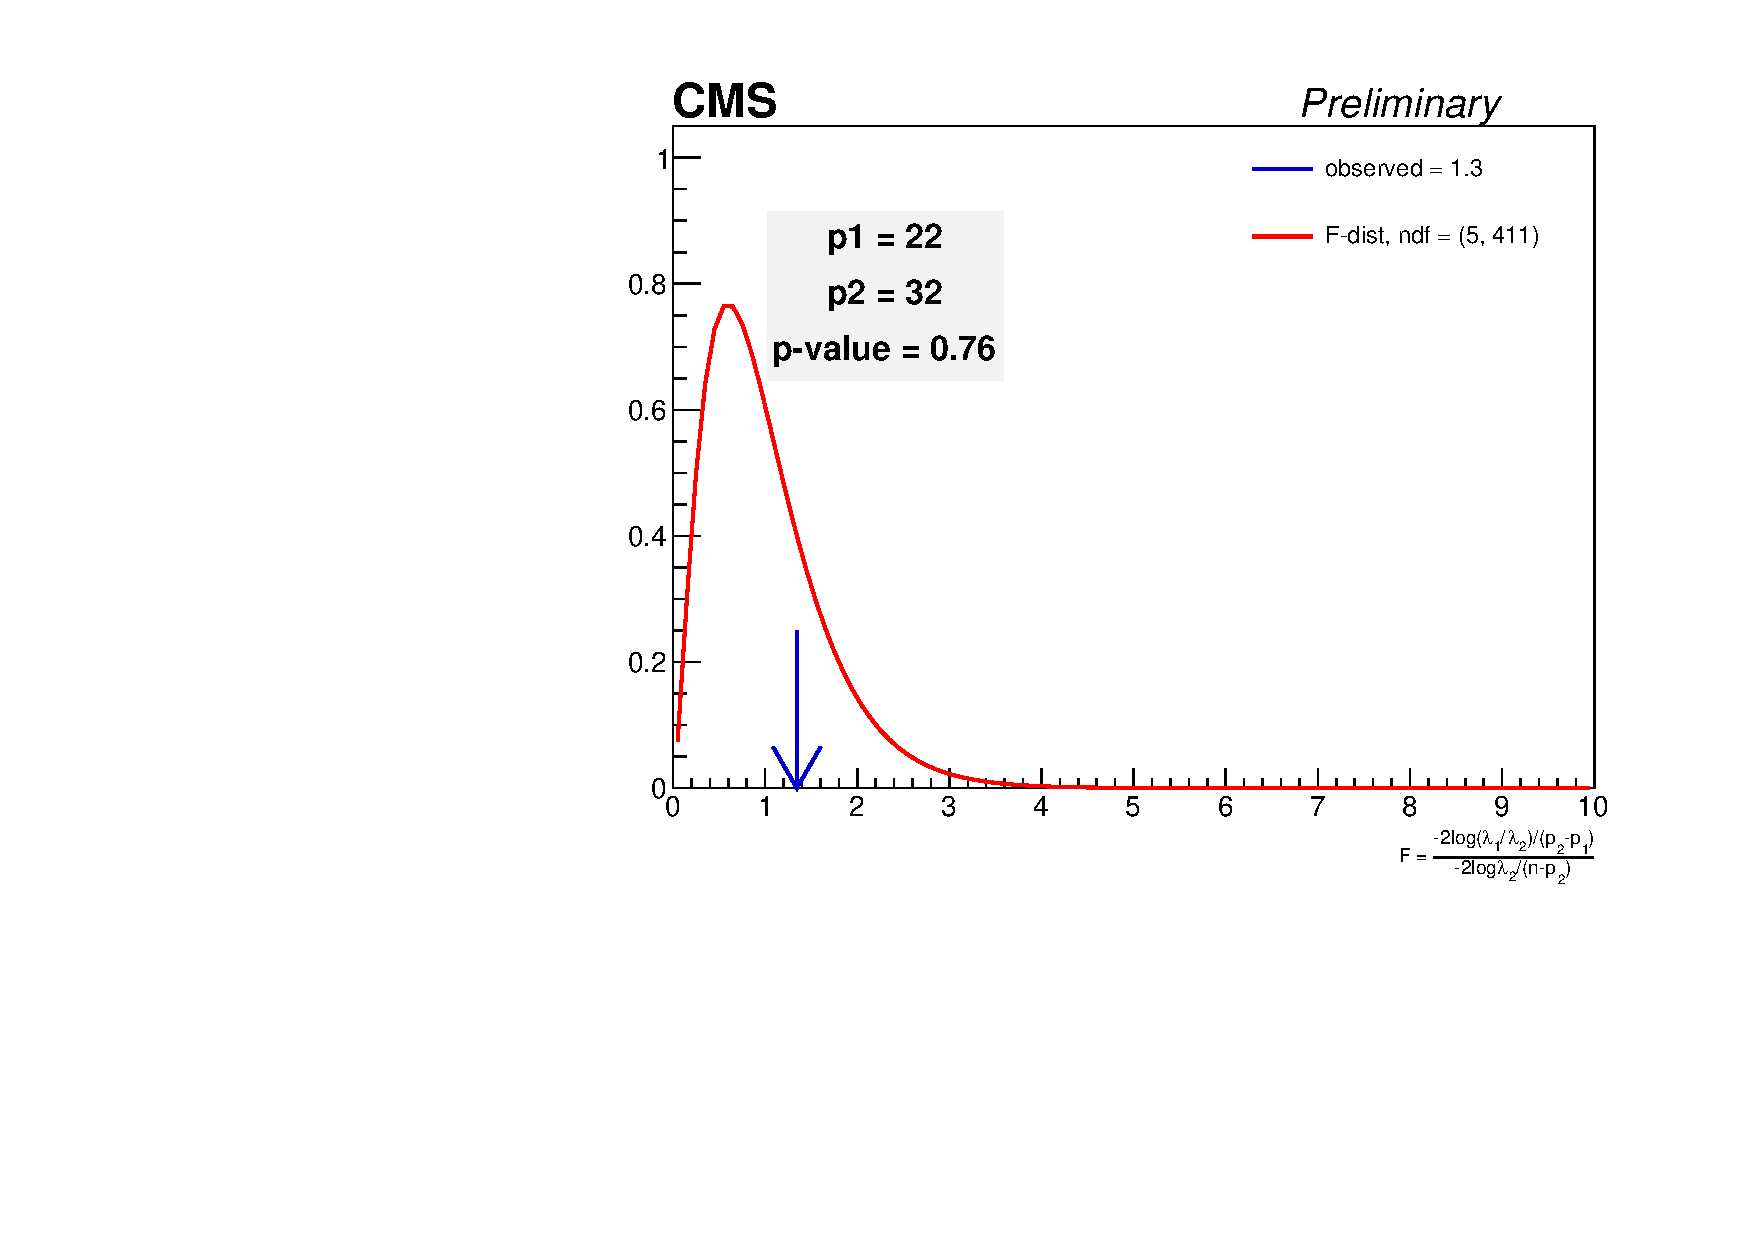
\includegraphics[width=0.4\textwidth]{Figures/ftest_vs_FTESTBNEWpol22_pol32_notoys.pdf}
	\caption{F-test plots showing that the 2x2 fit function is the most optimal. When reading these plot, p1 is the base fit function and p2 is the function that is being compared as an improvement. Whether for p1 or p2, the designation pol gives the 
	order of the polynomial fit function in $\mjred$, $\mred$ in order. Pol11 means 1st order polynomial in $\mjred$ and 1st order polynomial in $\mred$.}
	\label{fig:ftest_plots}
\end{figure} 
% \begin{figure}[!htb]
% 	\centering
% 	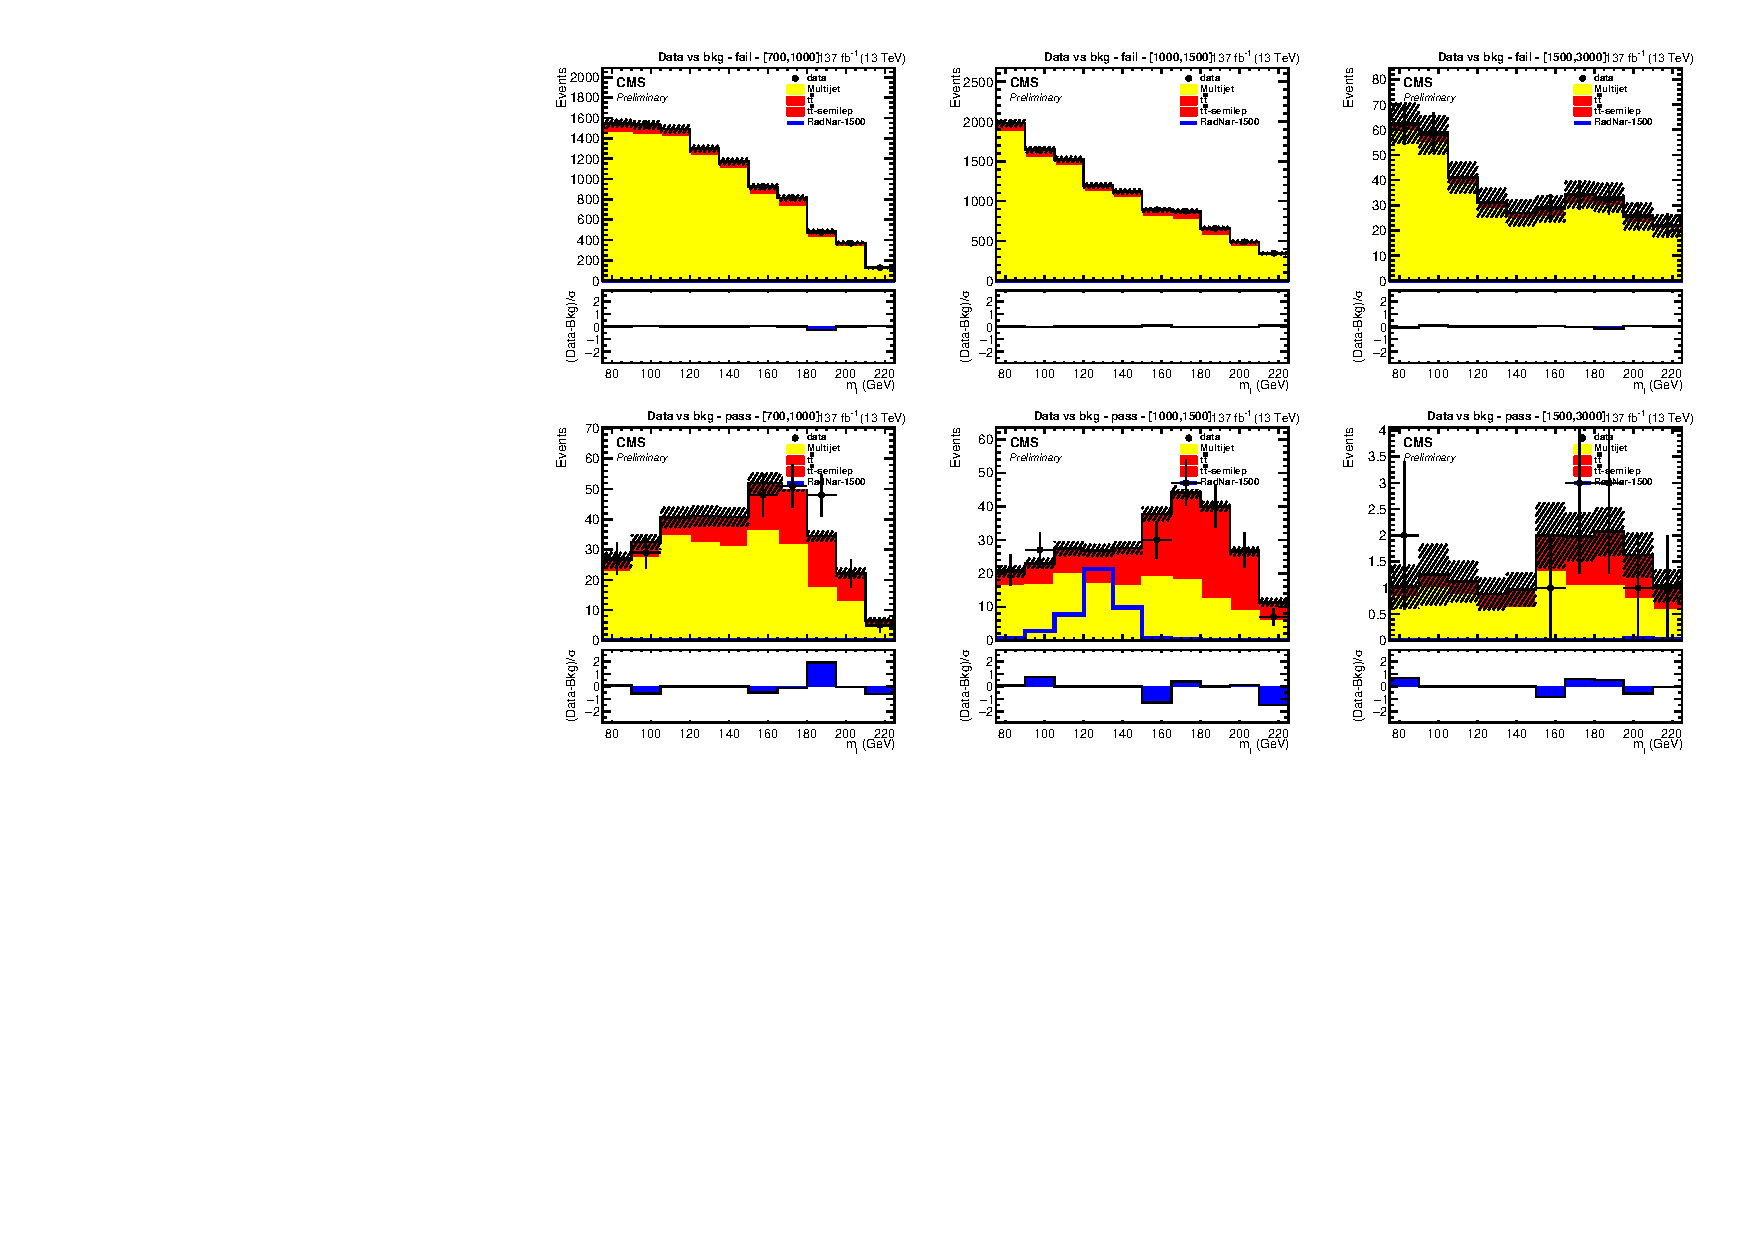
\includegraphics[width=1\textwidth]{Figures/postfit_projx_fitb_2x2TT.pdf}
% 	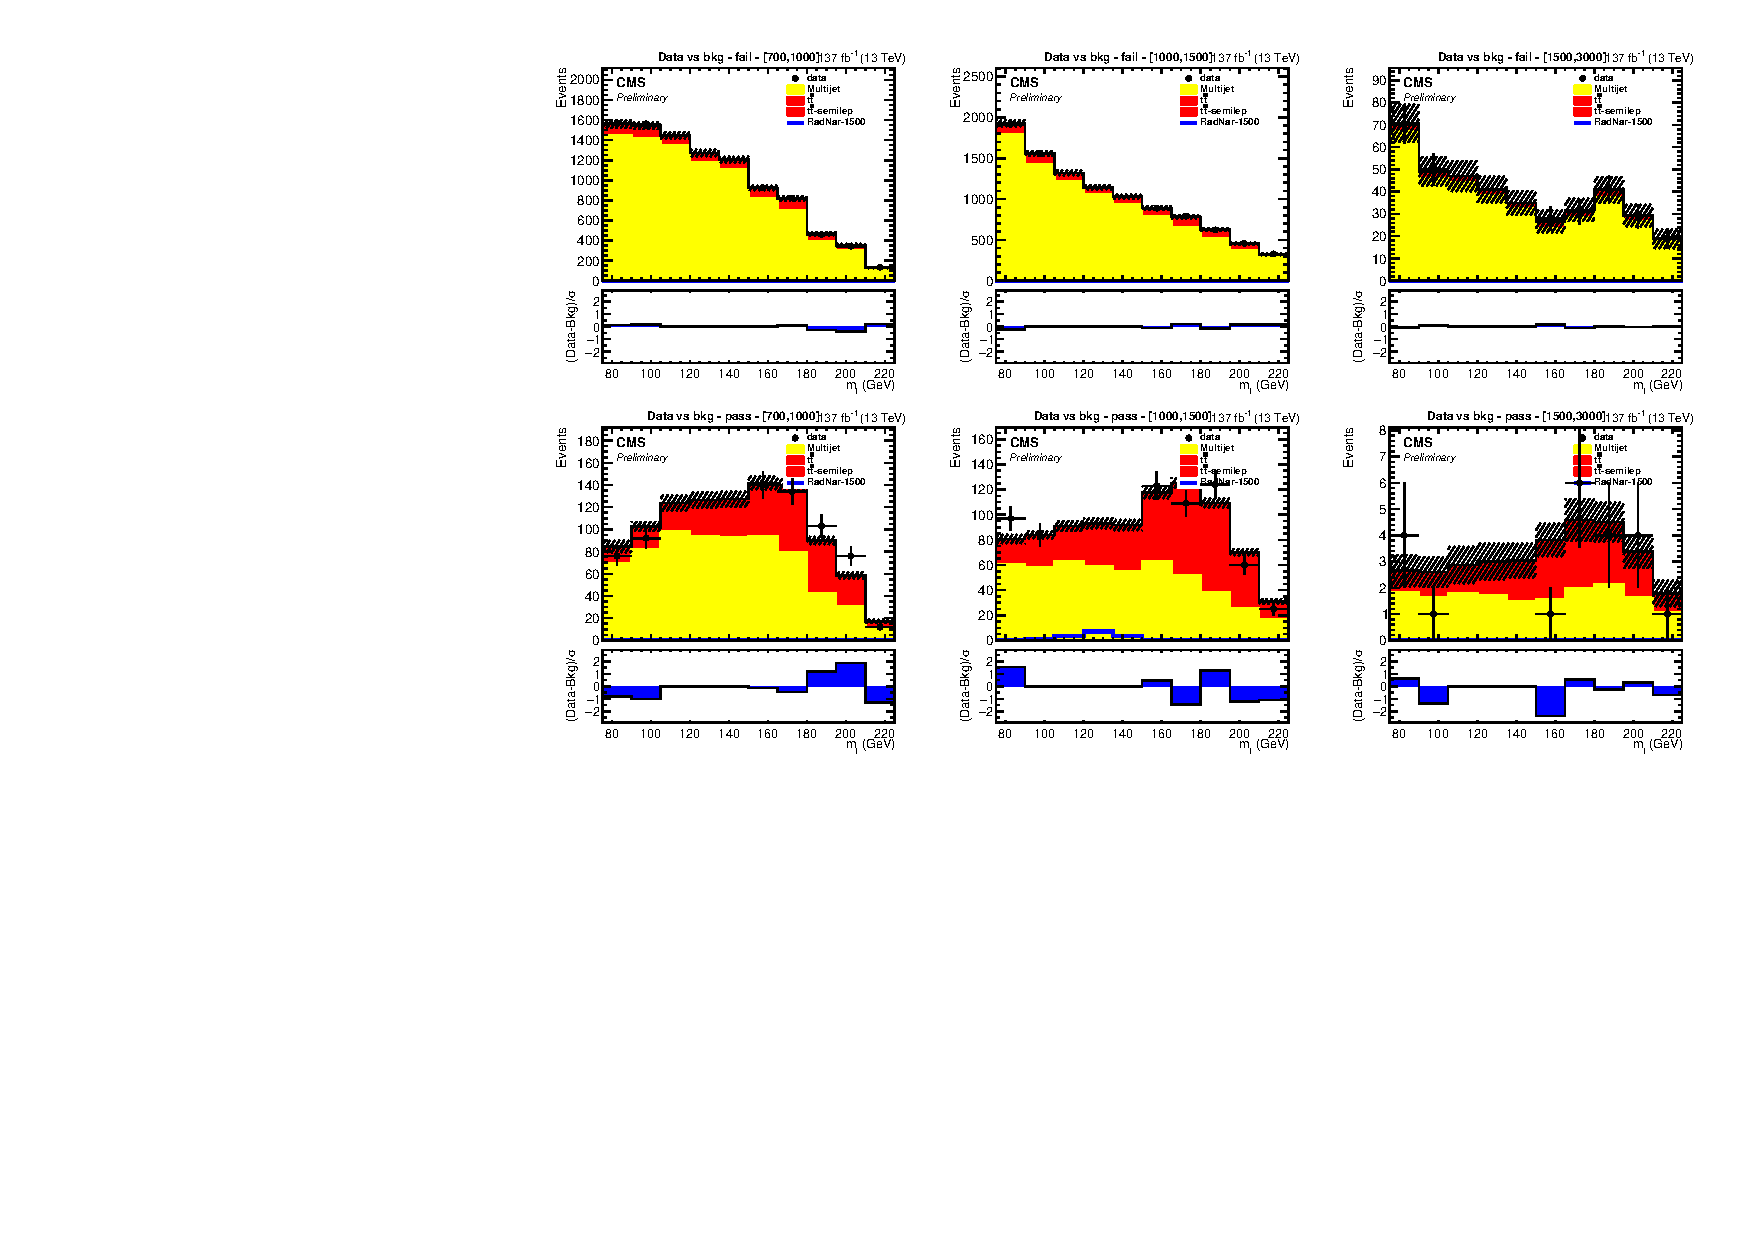
\includegraphics[width=1\textwidth]{Figures/postfit_projx_fitb_2x2LL.pdf}
% 	\caption{Full Run 2 Tight Tight background only fits for $M_j$ axis and $M_{jj}^{red}$ axis including expected Radion 1500 GeV signal, normalized to the signal strength found by the fit.}
% 	\label{fig:ftest_fits}
% \end{figure}
\clearpage
\section{2D Alphabet Validation Study}
We are interested in knowing how well the 2D Alphabet method compares to the previous method used in \cite{CMS-PAS-B2G-16-026}. Here we present multiple limits:
\begin{itemize}
	\item The 2016 Double B tagger limit from \cite{CMS-PAS-B2G-16-026}.
	\item The 2016 Double B tagger limit made by using 2Dalphabet in 1D and including the $\tau_{21}$ cut.
	% \item The 2016 Double B tagger limit from \cite{CMS-PAS-B2G-16-026} but scaled by $\sqrt(luminosity)$.
	\item The 2016 Double B Tagger limit made with 2D Alphabet.
	\item The full run 2 Double B Tagger limit made with 2D Alphabet
	\item The full run 2 dak8MDHbb limit made with 2D Alphabet
\end{itemize}
We present the comparison in the following plot:
\begin{figure}[!htb]
	\centering
	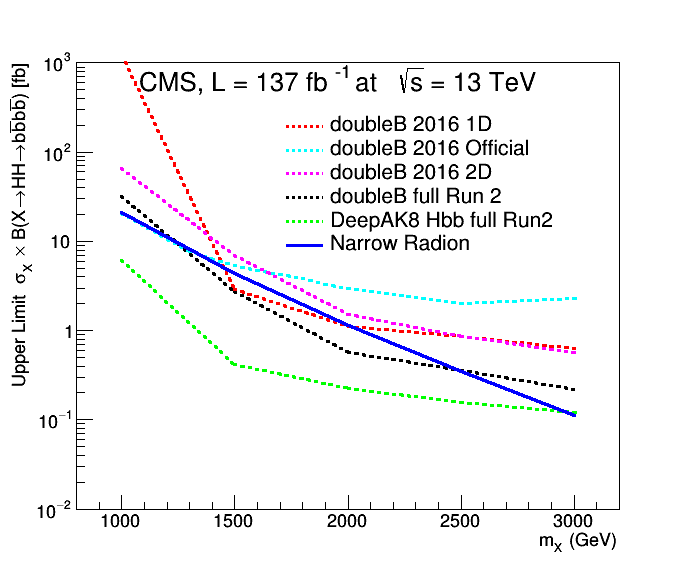
\includegraphics[width=0.5\textwidth]{Figures/limits_HH_combine_137fb_fullrun2_limit_comparison_RadNar.png}
	\caption{Comparison plot of various limits.}
	\label{fig:compplot}
\end{figure}
\section{Example Combine Card}
The combine cards for this analysis are stored in git and may be viewed here: \\
\url{https://github.com/dbrehm/JHUanalyzer/tree/rdfHH4b/Framework/AnalysisModules/B2G-20-004/DataCards}

\section{$\tau_{21}$ Study}
We studied the effect of the $\tau_{21}$ cut used in the original analysis. We plot the results of this study:
\begin{figure}[!htb]
	\centering
	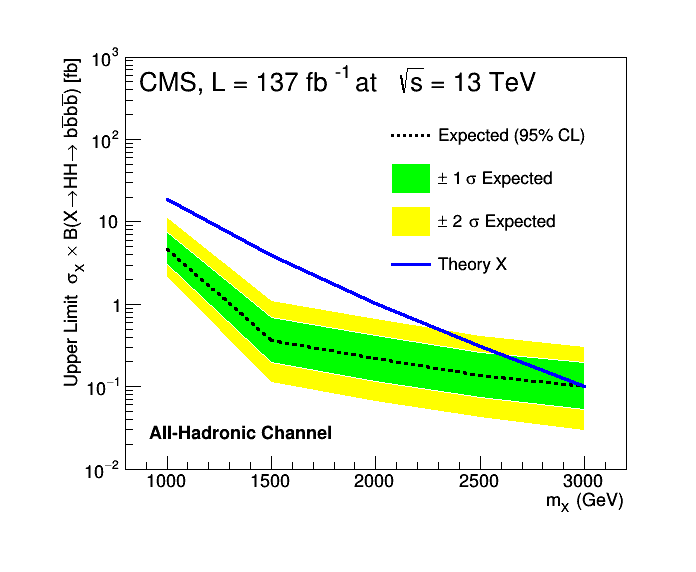
\includegraphics[width=0.4\textwidth]{Figures/limits_combine_137fb_dak8MDHbb_signalsAll_RadNar_750rmcut_yestau21.png}
	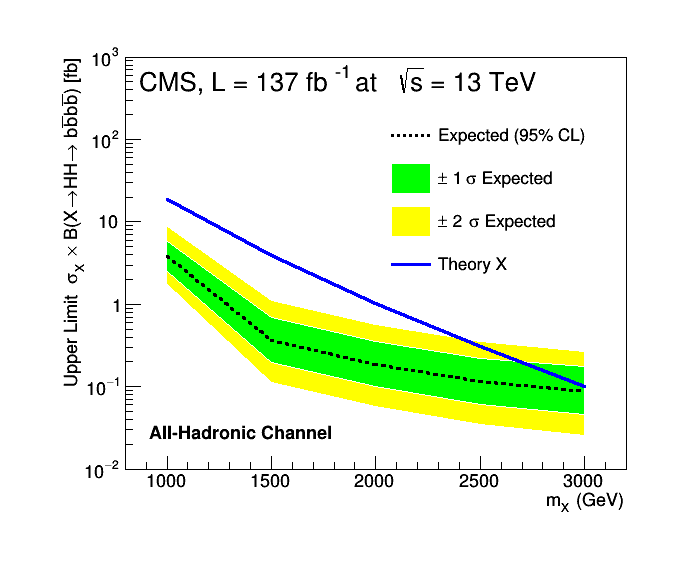
\includegraphics[width=0.4\textwidth]{Figures/limits_combine_137fb_dak8MDHbb_signalsAll_RadNar_750rmcut_notau21.png}
	\caption{Comparison of limits with and without $\tau_{21}$ cut. The plot on the right is with the cut and the plot on the left is without the cut.}
	\label{fig:tau21study}
\end{figure}
It is easy to see here that there is very little difference in the above plots. This is helpful because we then gain on statistics and systematic uncertainties as the $\tau_{21}$ scale factor uncertainty is not applied to the above limit plots.
\pagebreak
\section{By Year Fits}
Previous version of this analysis fit each year by itself. The current version of the fitting procedure combined each year so that there are only the three regions to be fit. These are the plots generated when the fit was done by year. 
\\
\textbf{These plots don't necessarily correspond to the latest fixes/updates/optimizations that were made to the full run 2 fit. Until we are able to confirm that the by year fit can happen with our latest methodology, the plots in this
section should be considered to be in need of fixing.} \\
% \subsection{Closure Test in Data\label{ss:BkgValInDataByYear}}
% \begin{figure}[!htb]
% 	\centering
% 	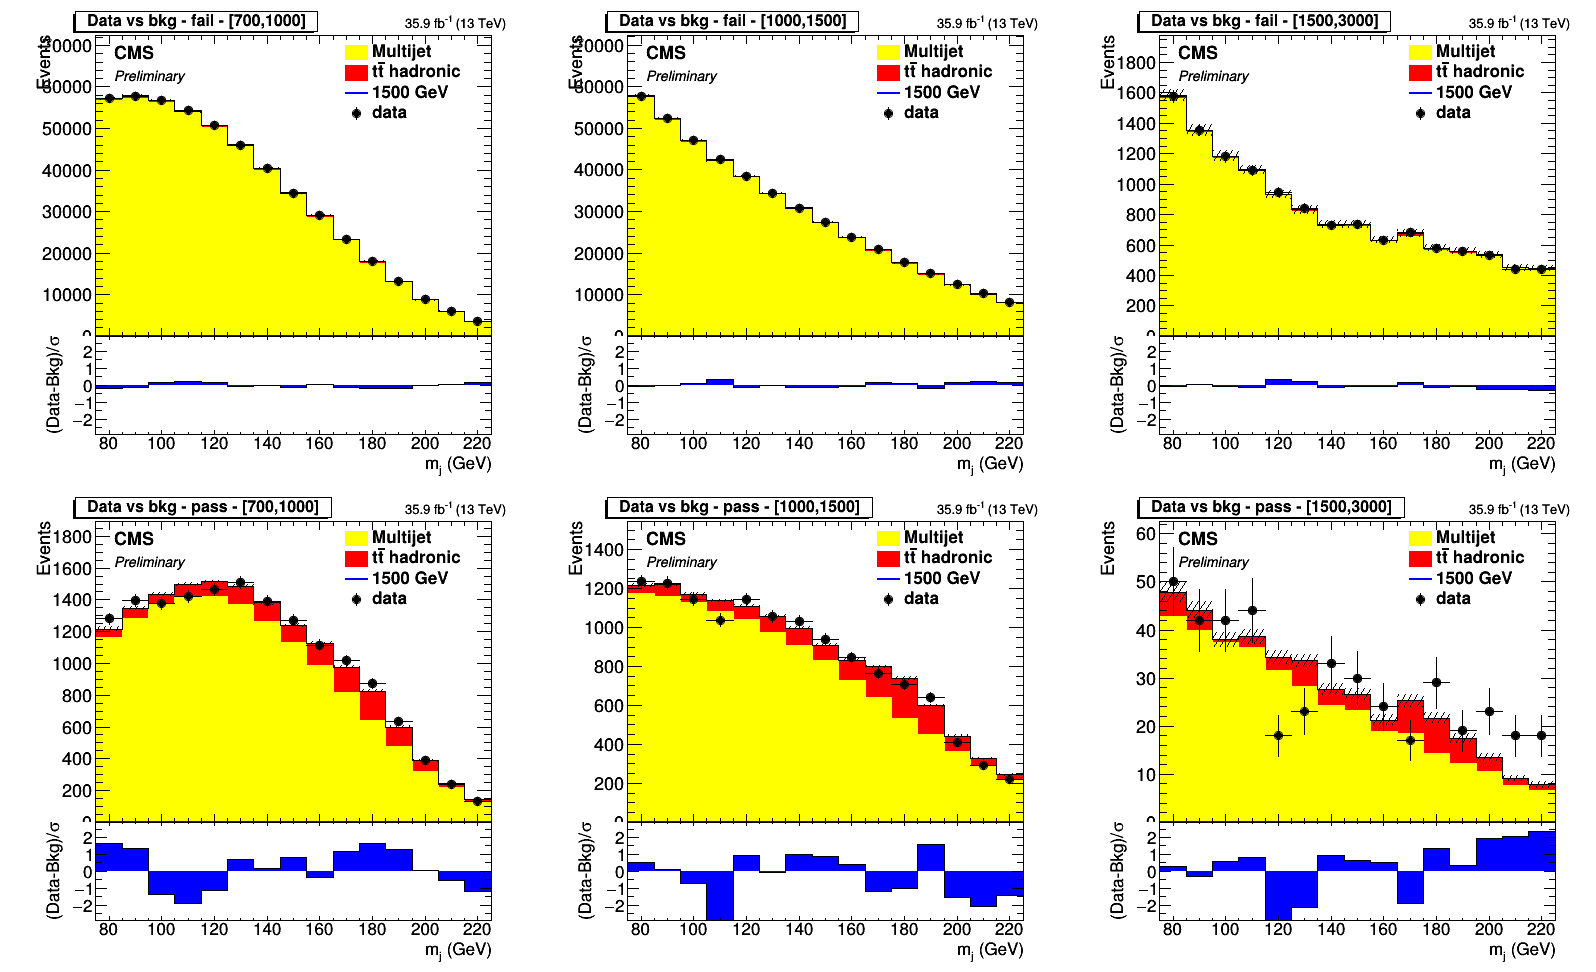
\includegraphics[width=1\textwidth]{Figures/postfit_projx_fitb_16CR.png}
% 	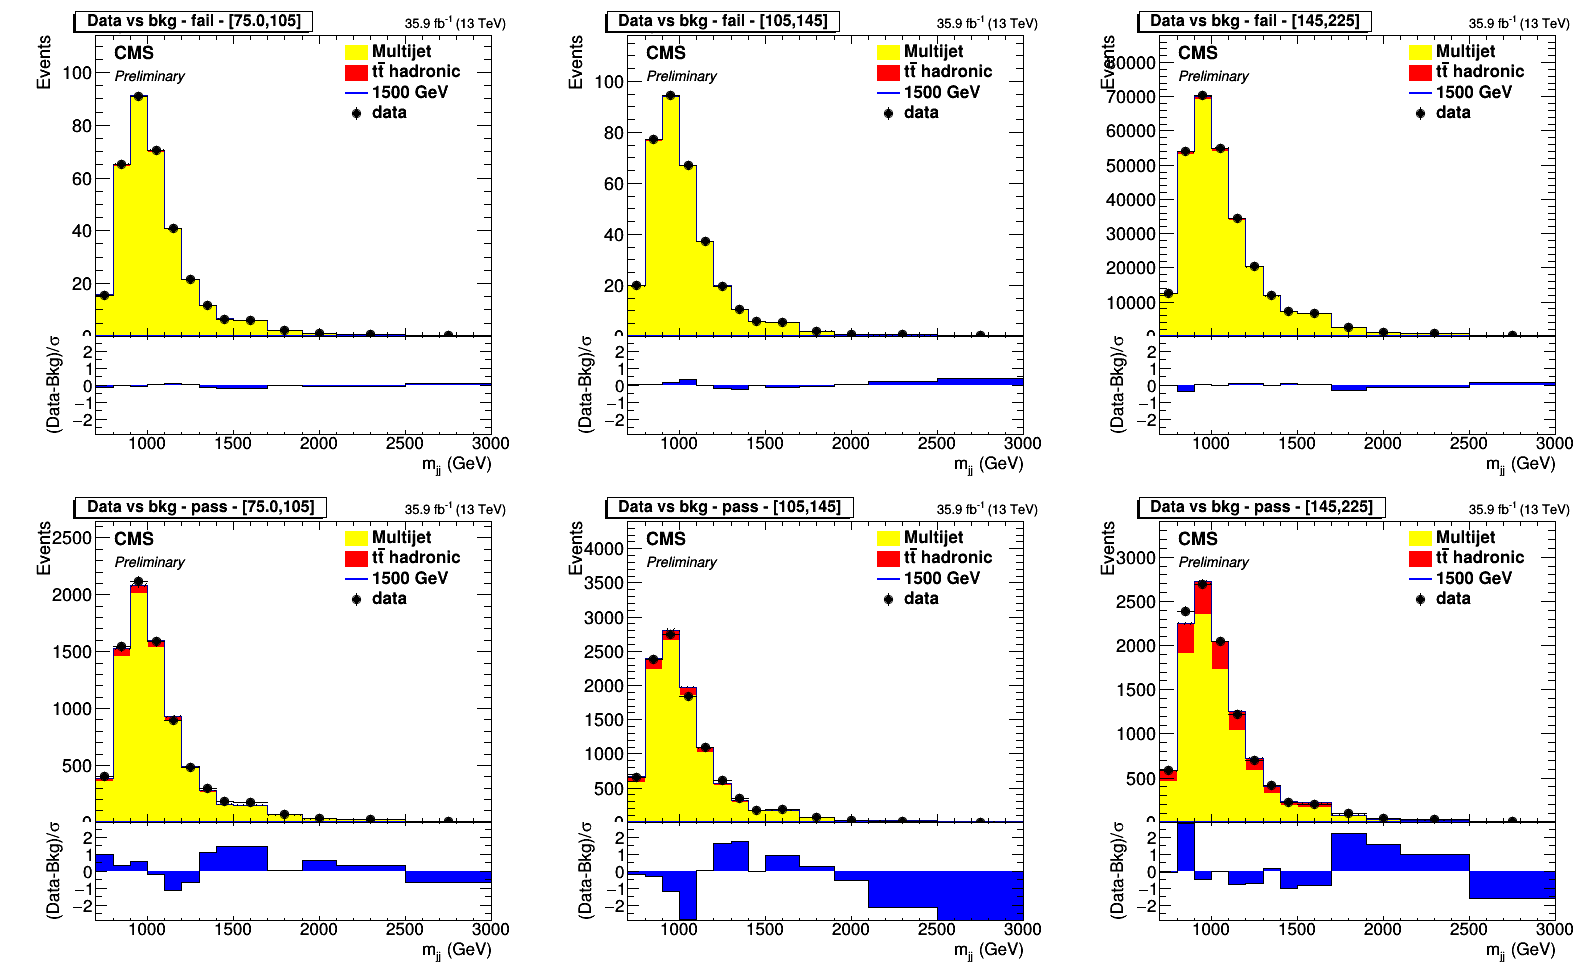
\includegraphics[width=1\textwidth]{Figures/postfit_projy_fitb_16CR.png}
% 	\caption{2016 CR fits for $M_j$ axis and $M_{jj}$ axis.}
% 	\label{fig:16CR}
% \end{figure}
% \begin{figure}[!htb]
% 	\centering
% 	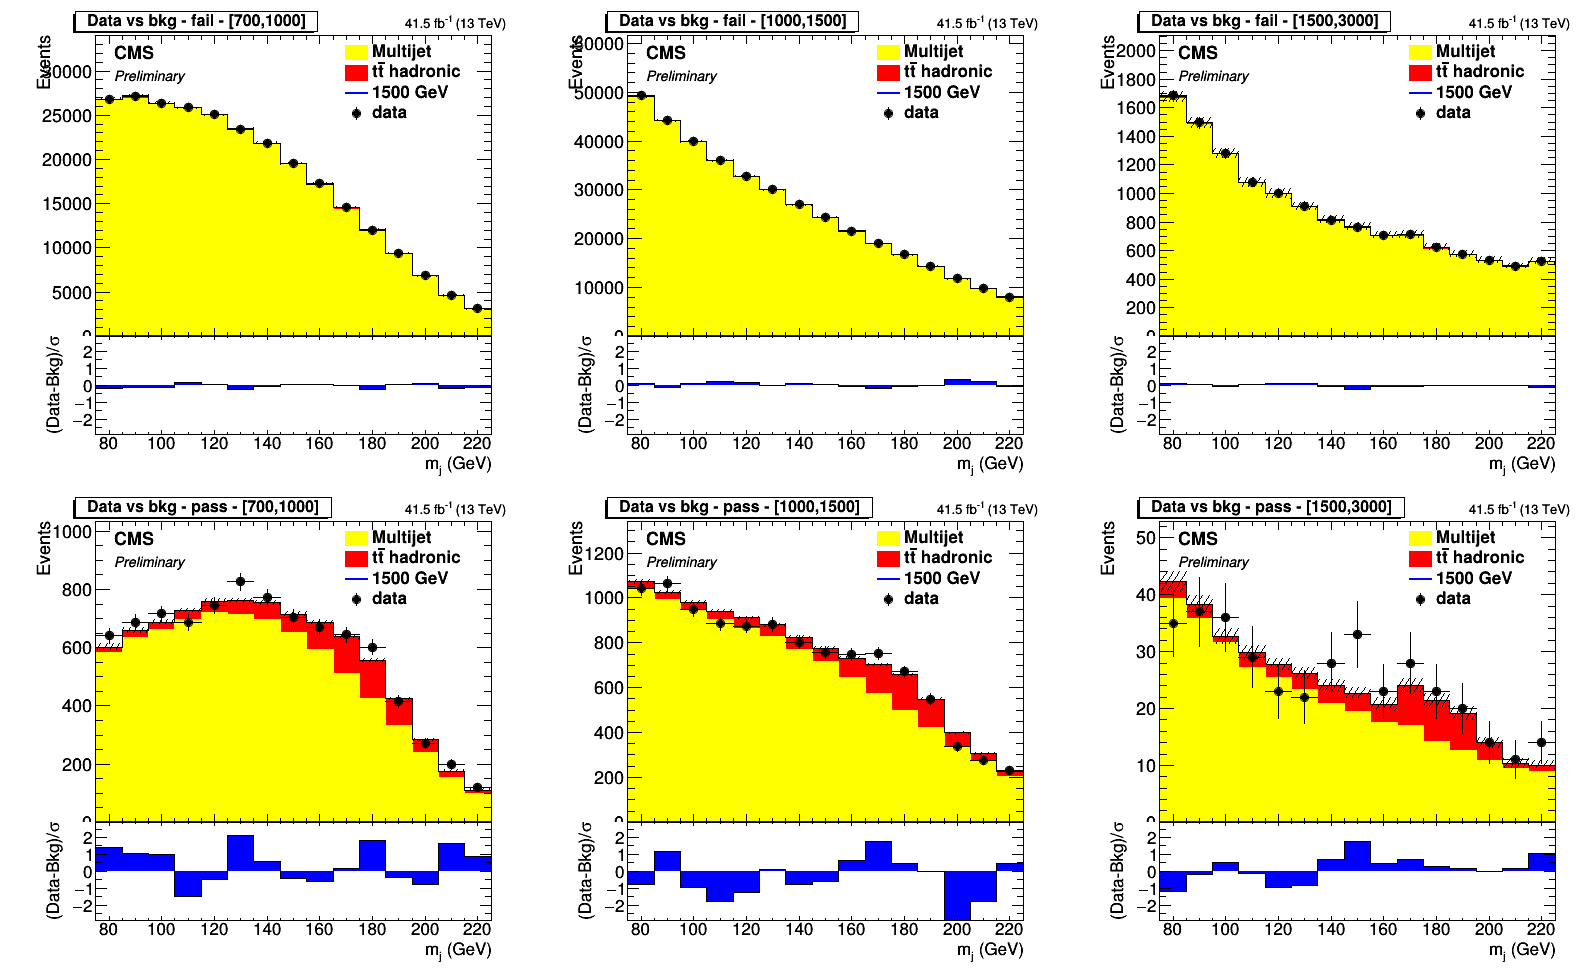
\includegraphics[width=1\textwidth]{Figures/postfit_projx_fitb_17CR.png}
% 	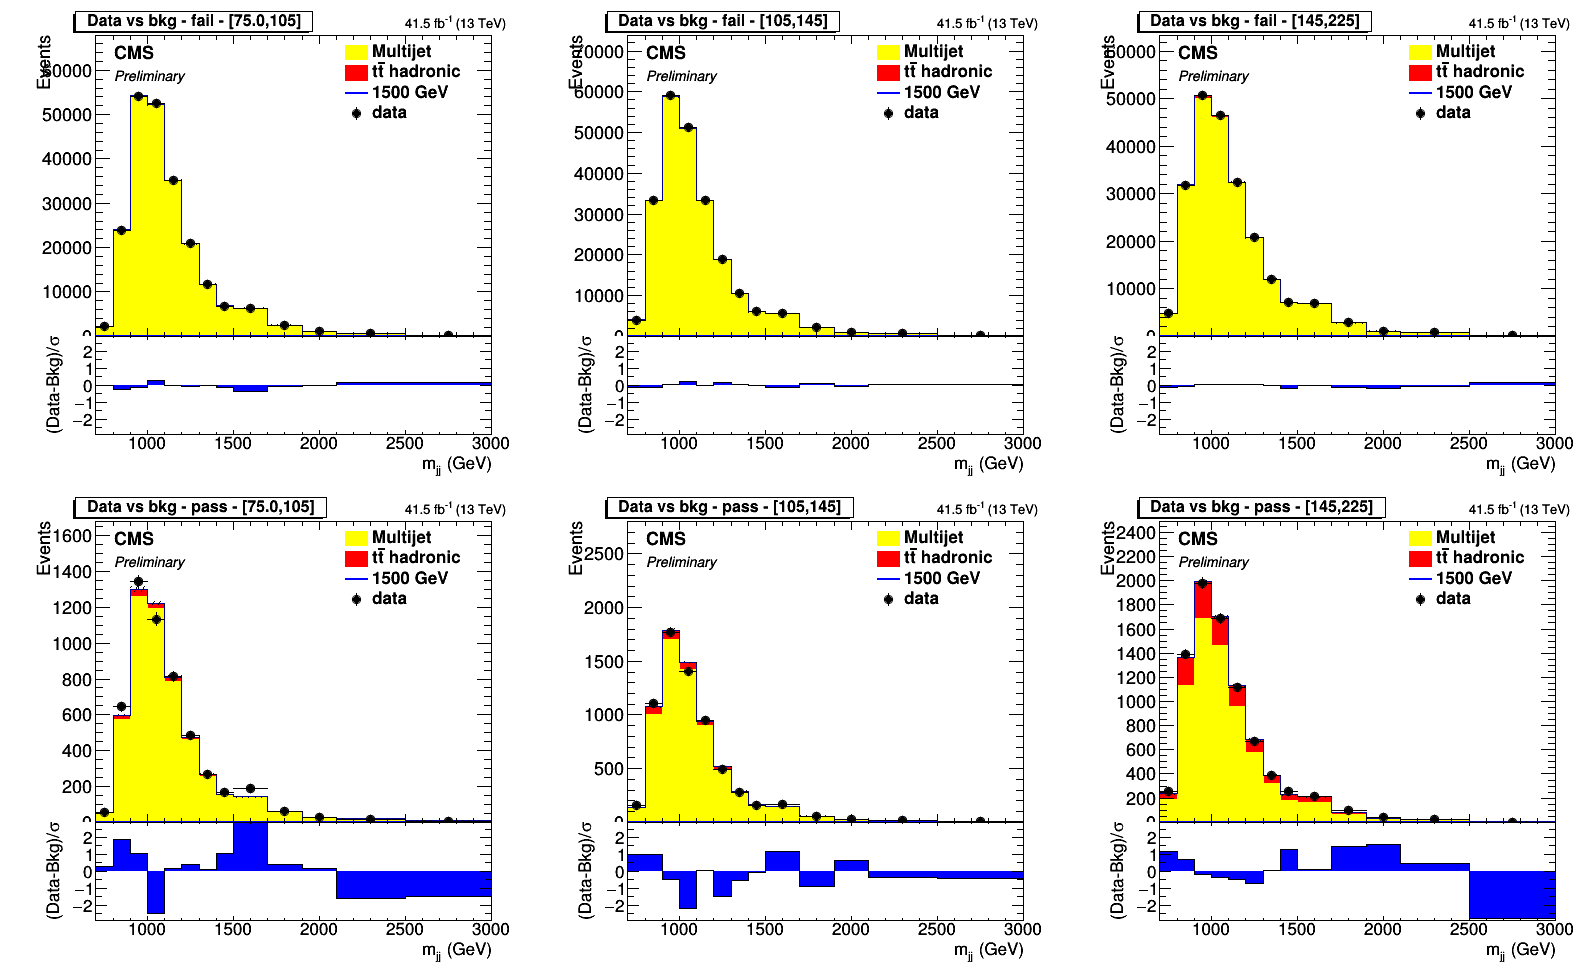
\includegraphics[width=1\textwidth]{Figures/postfit_projy_fitb_17CR.png}
% 	\caption{2017 CR background fits for $M_j$ axis and $M_{jj}$ axis.}
% 	\label{fig:17CR}
% \end{figure}
% \begin{figure}[!htb]
% 	\centering
% 	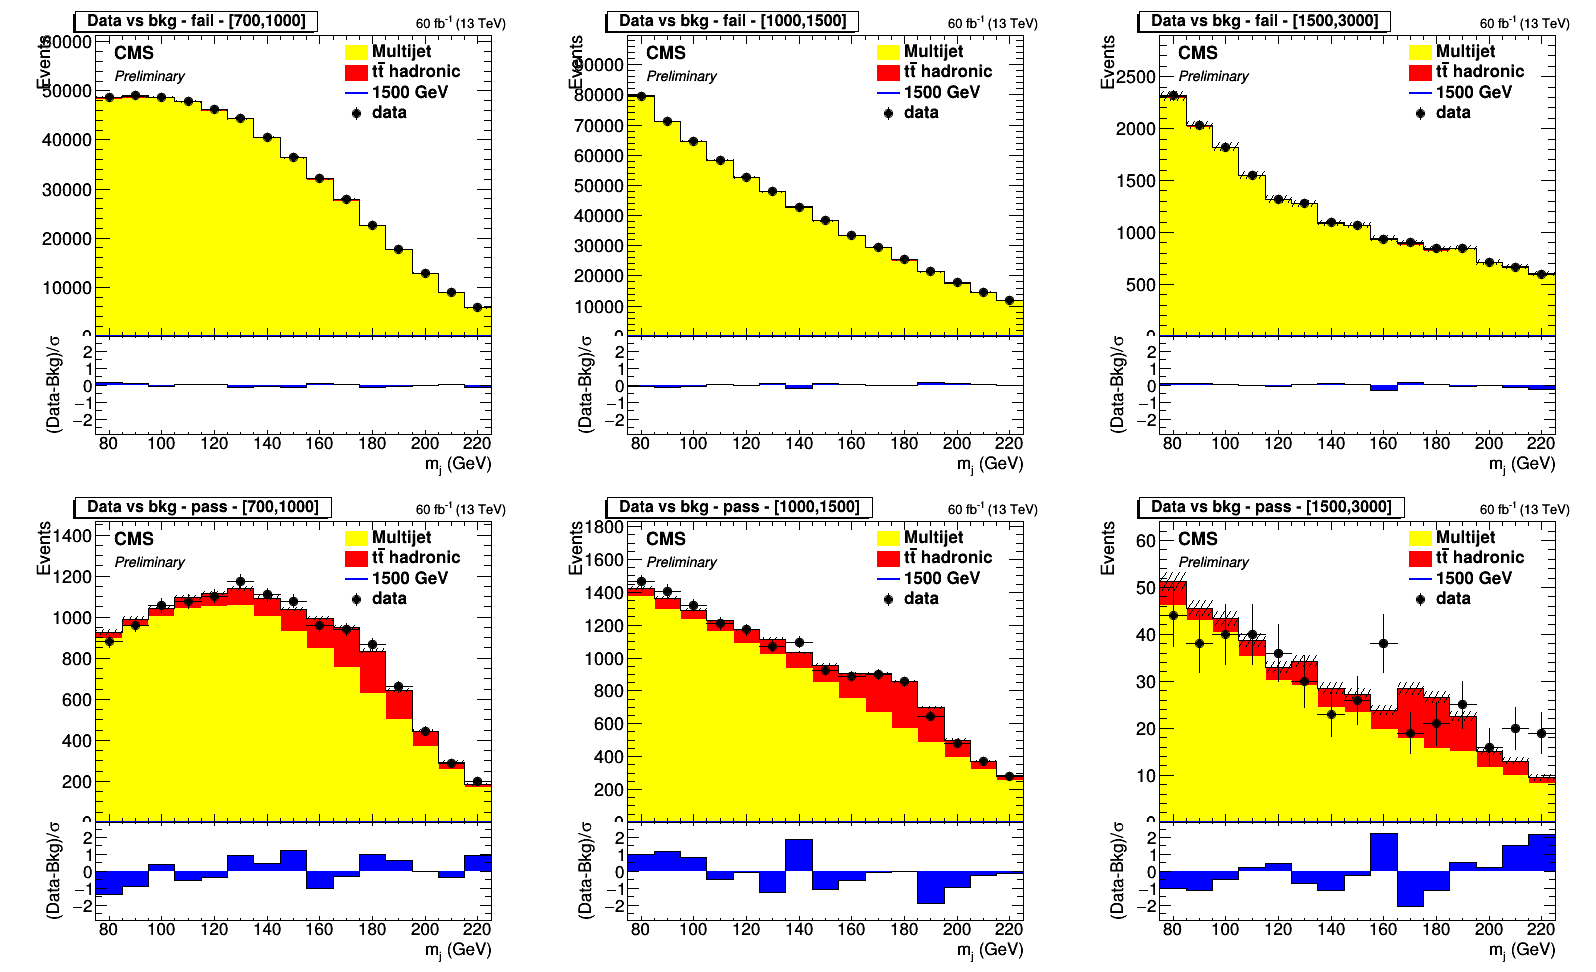
\includegraphics[width=1\textwidth]{Figures/postfit_projx_fitb_18CR.png}
% 	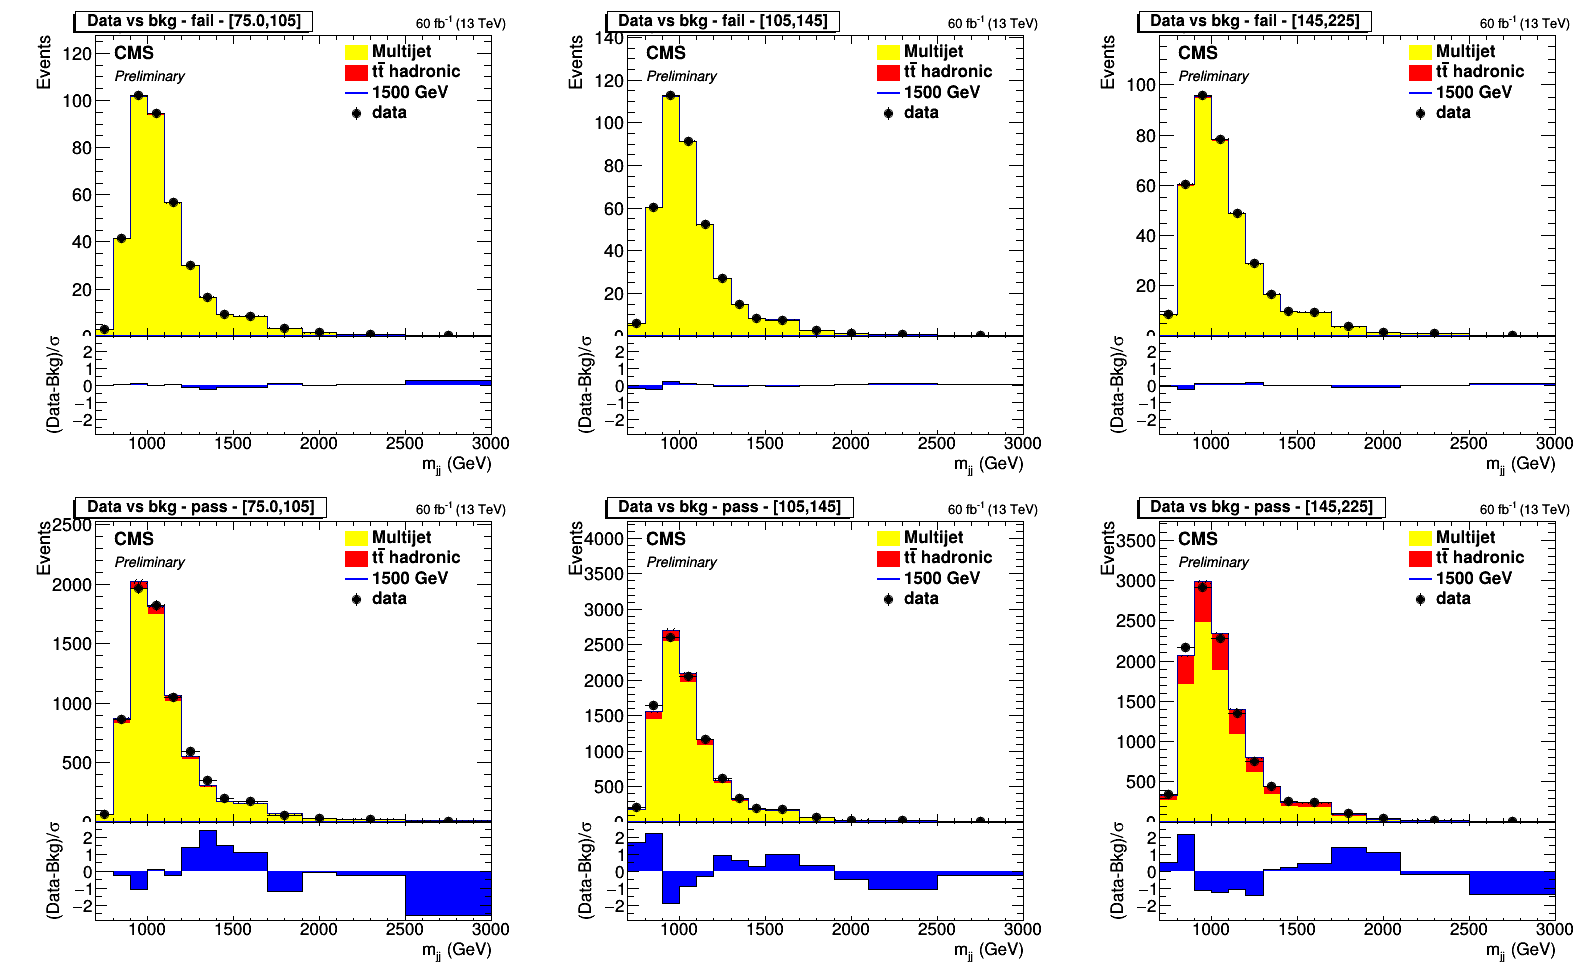
\includegraphics[width=1\textwidth]{Figures/postfit_projy_fitb_18CR.png}
% 	\caption{2018 CR background fits for $M_j$ axis and $M_{jj}$ axis.}
% 	\label{fig:18CR}
% \end{figure}
\subsection{Signal Regions Prediction By Year\label{ss:BkgInSigRegionByYear}}
\begin{figure}[!htb]
	\centering
	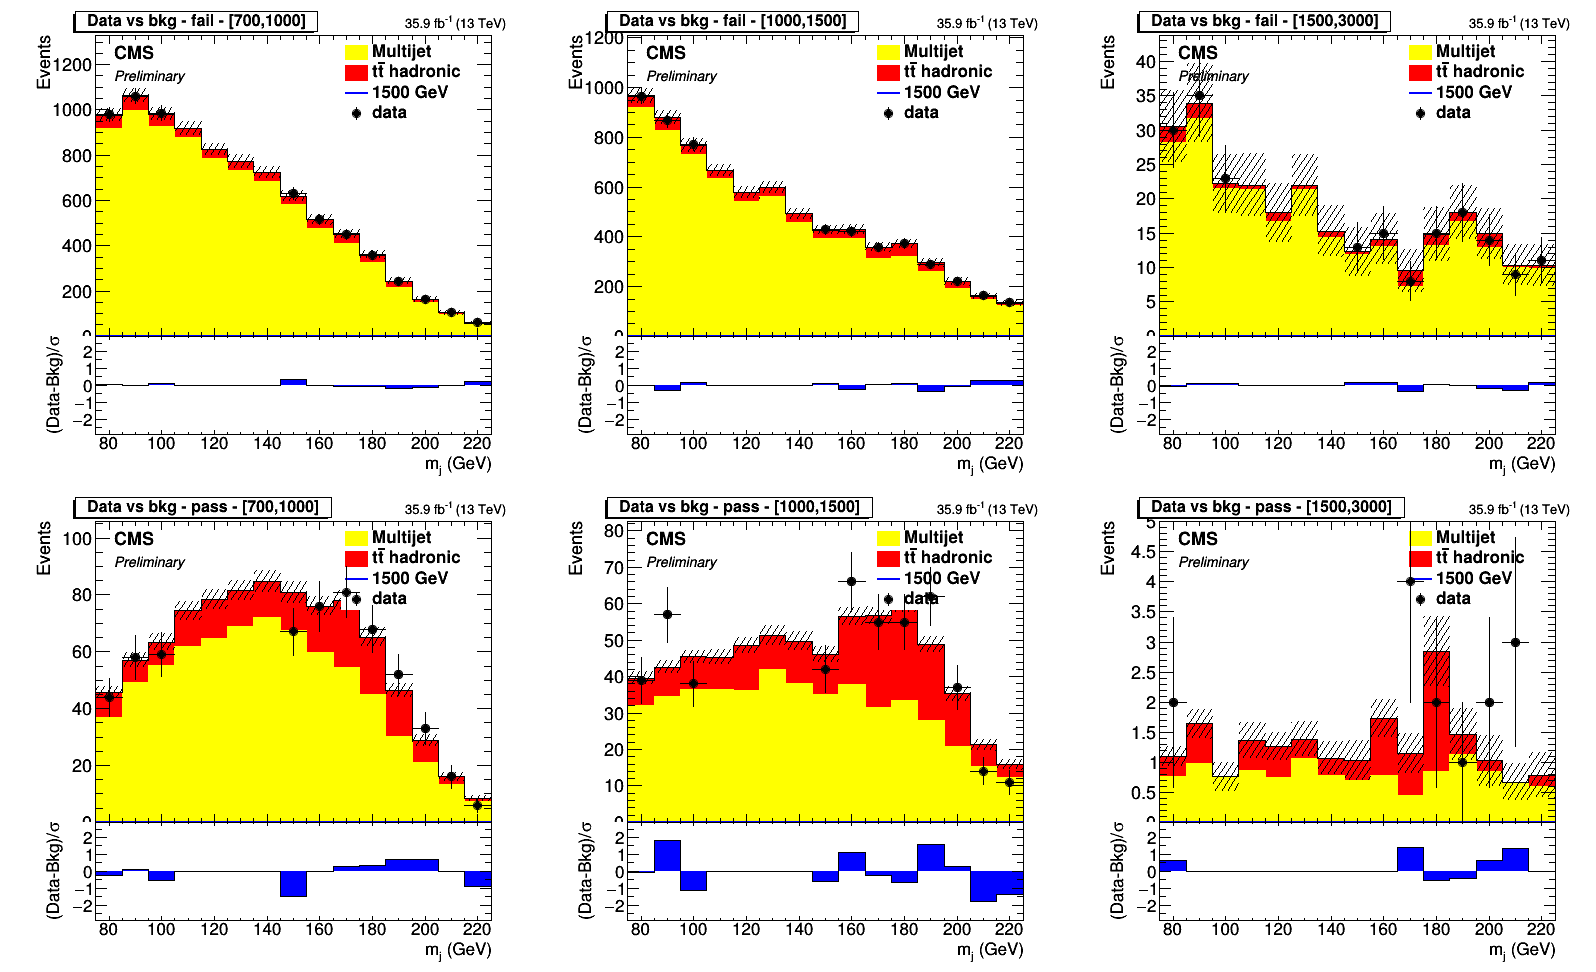
\includegraphics[width=1\textwidth]{Figures/postfit_projx_fits_16LL.png}
	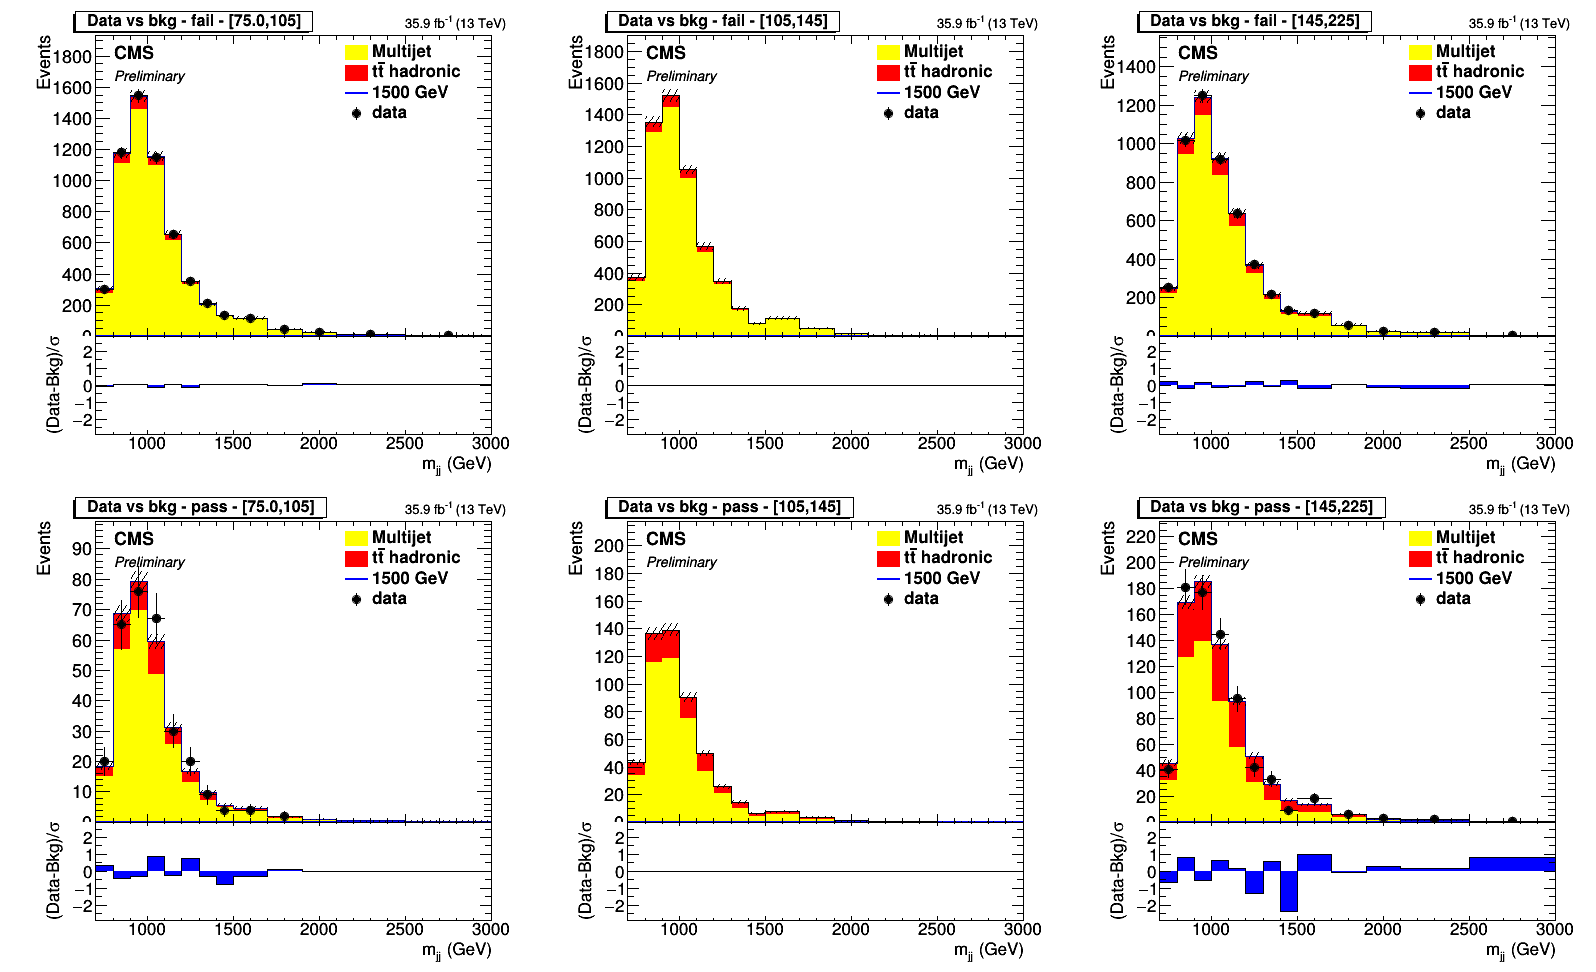
\includegraphics[width=1\textwidth]{Figures/postfit_projy_fits_16LL.png}
	\caption{2016 Loose Loose background fits for $M_j$ axis and $M_{jj}^{red}$ axis including expected Radion 1500 GeV signal, normalized to the signal strength found by the fit.}
	\label{fig:16LL}
\end{figure}
\begin{figure}[!htb]
	\centering
	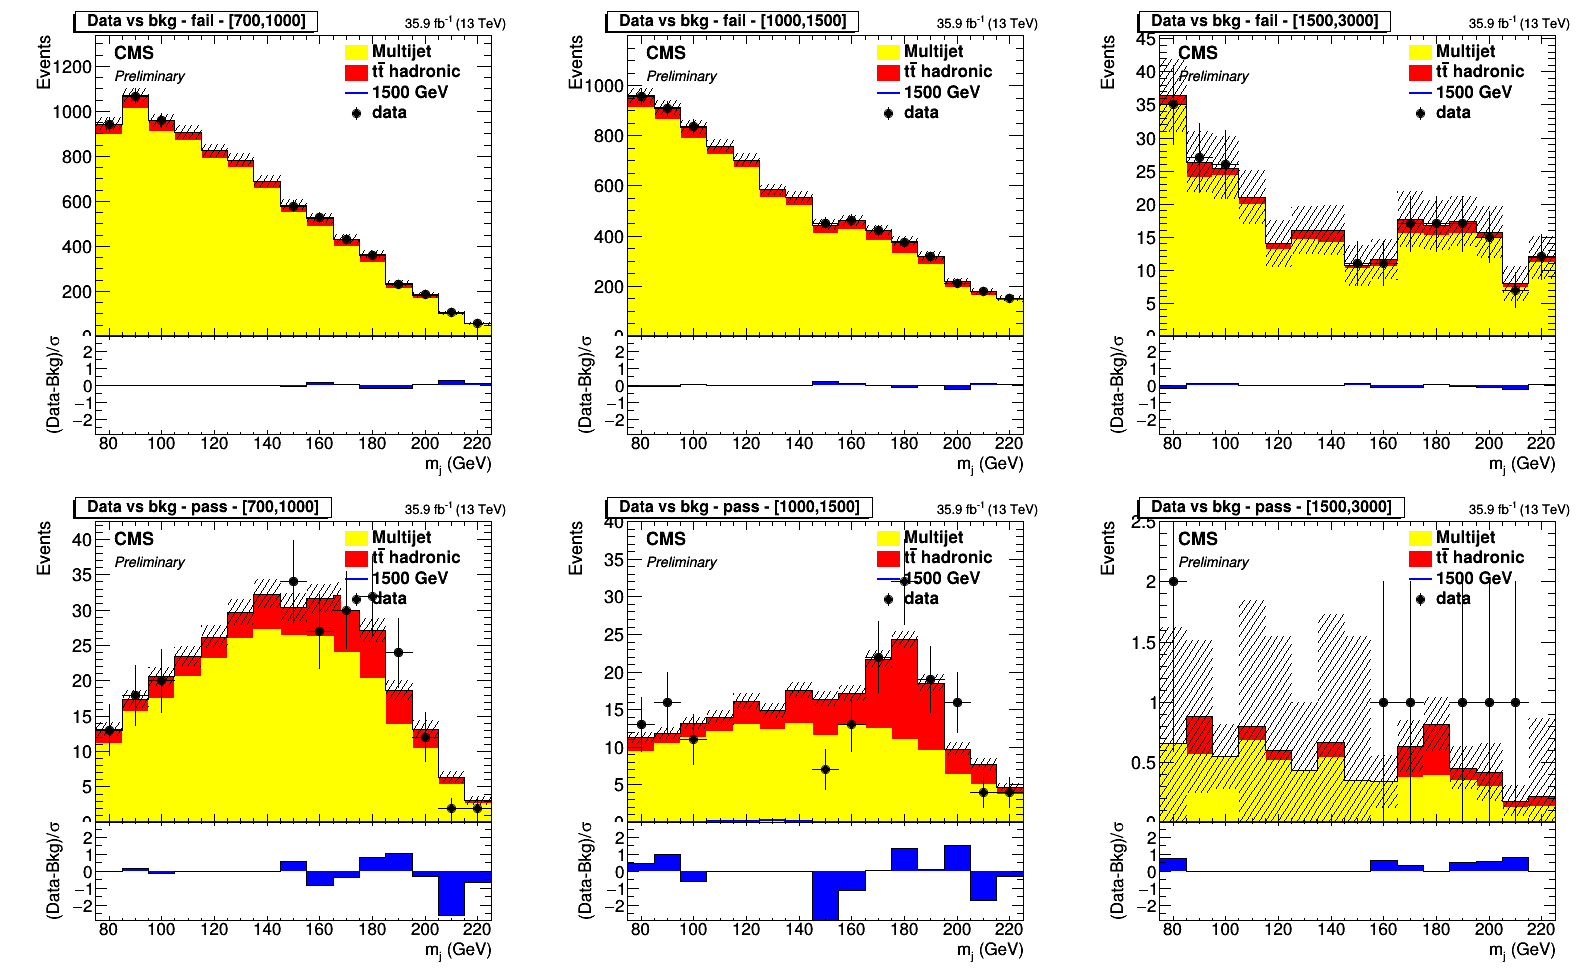
\includegraphics[width=1\textwidth]{Figures/postfit_projx_fits_16TT.png}
	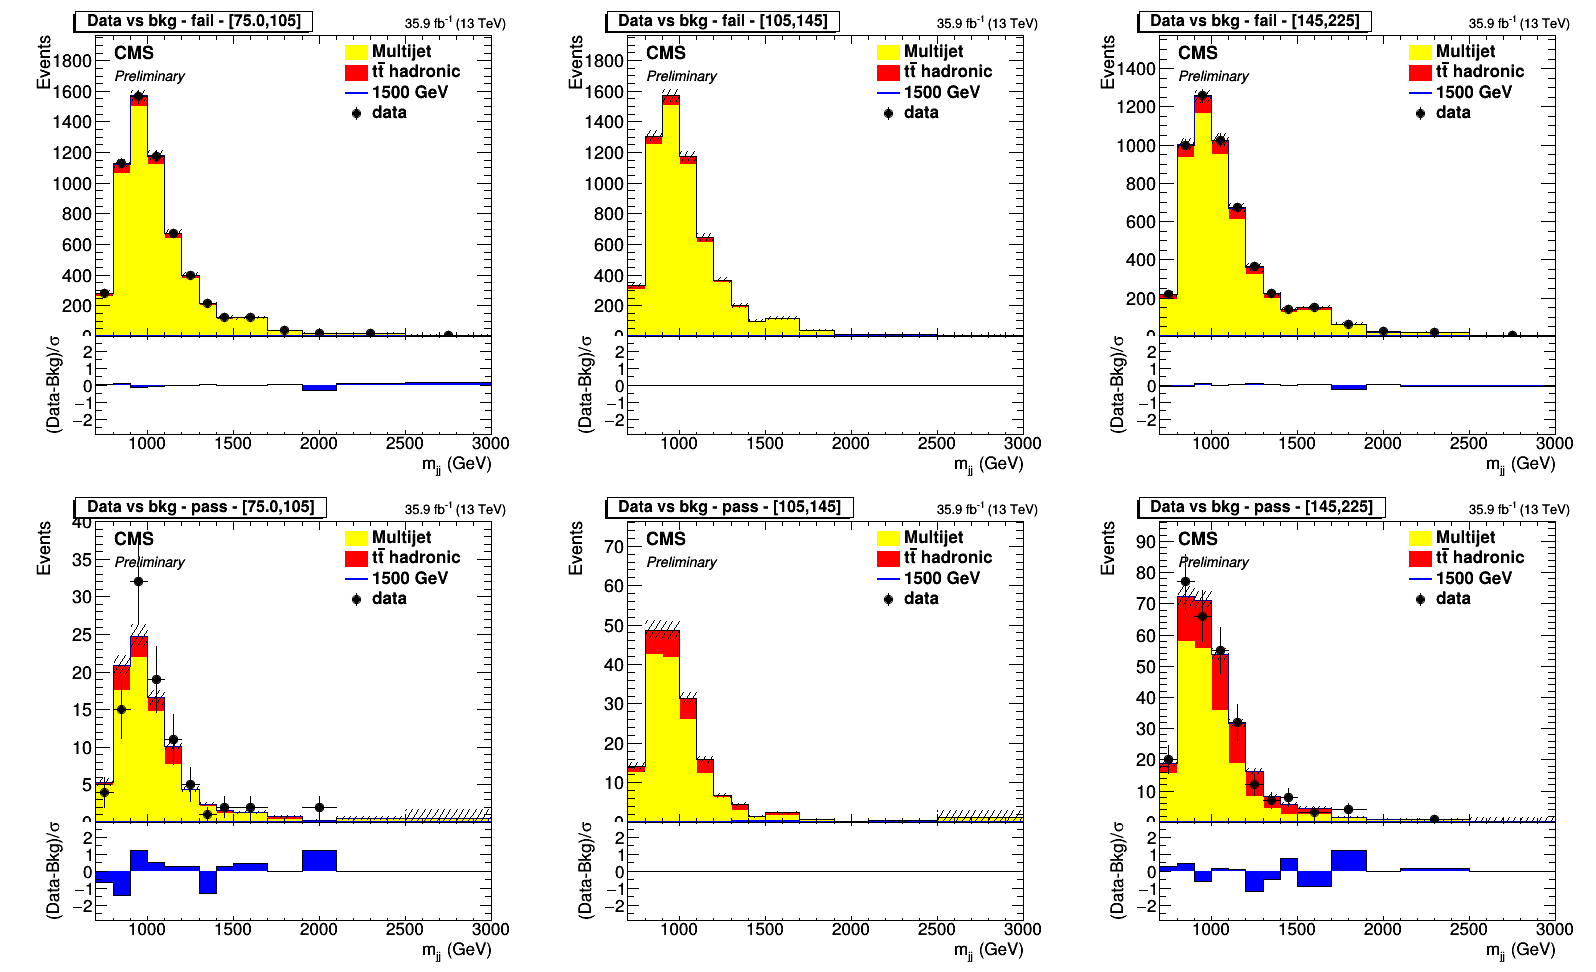
\includegraphics[width=1\textwidth]{Figures/postfit_projy_fits_16TT.png}
	\caption{2016 Tight Tight background fits for $M_j$ axis and $M_{jj}^{red}$ axis including expected Radion 1500 GeV signal, normalized to the signal strength found by the fit.}
	\label{fig:16TT}
\end{figure}
\begin{figure}[!htb]
	\centering
	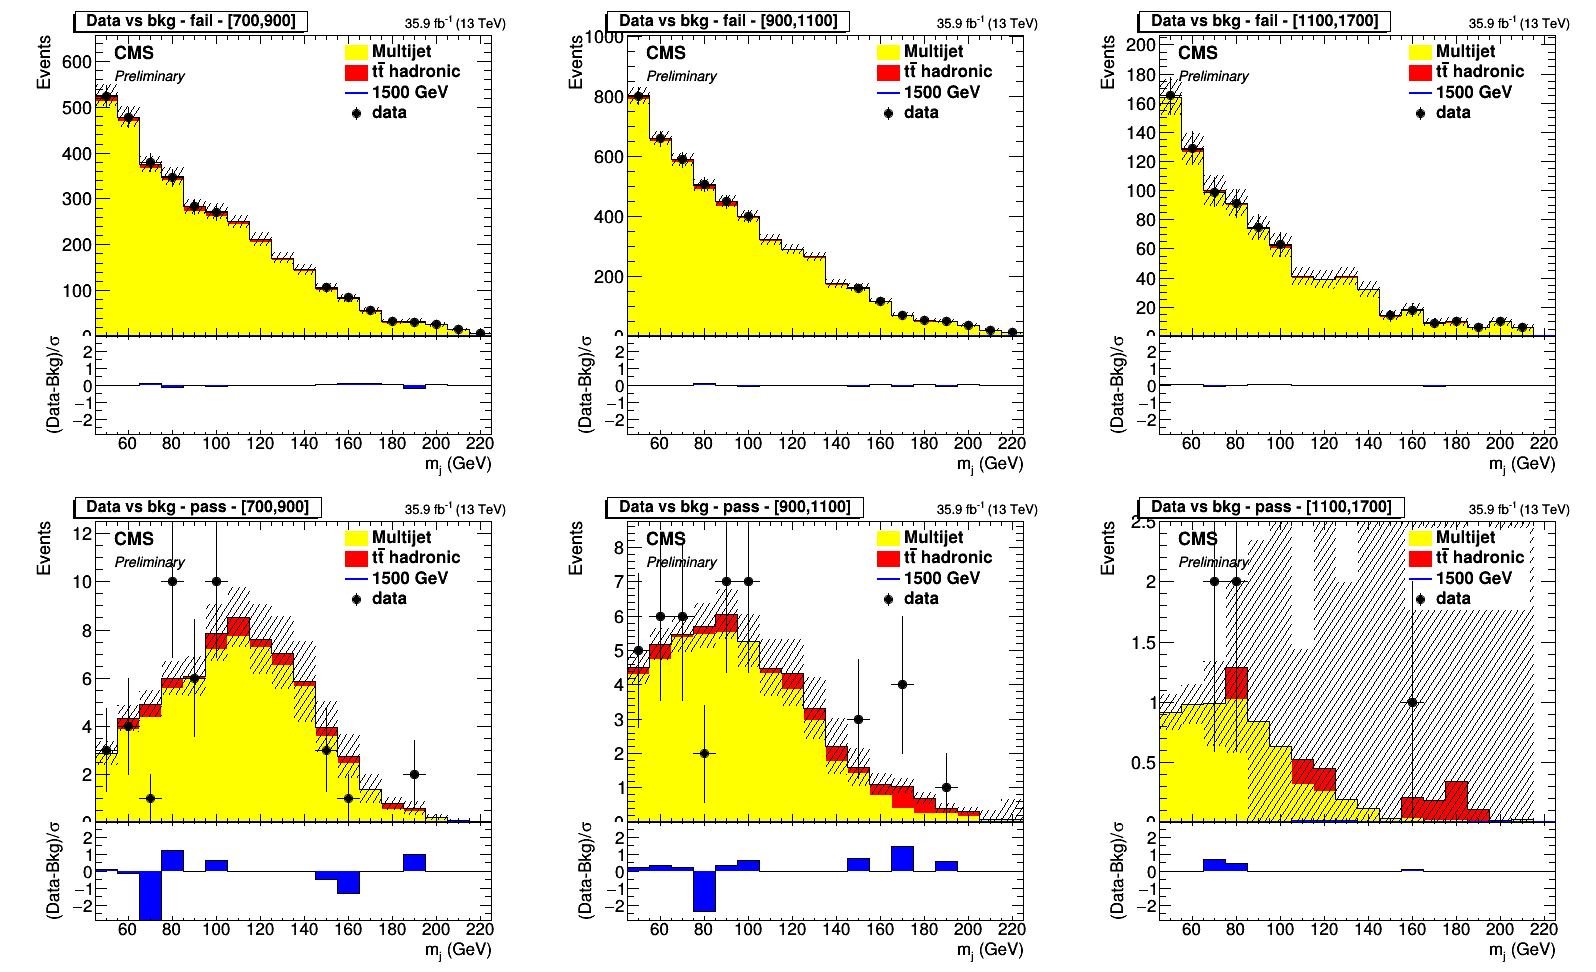
\includegraphics[width=1\textwidth]{Figures/postfit_projx_fits_1621.png}
	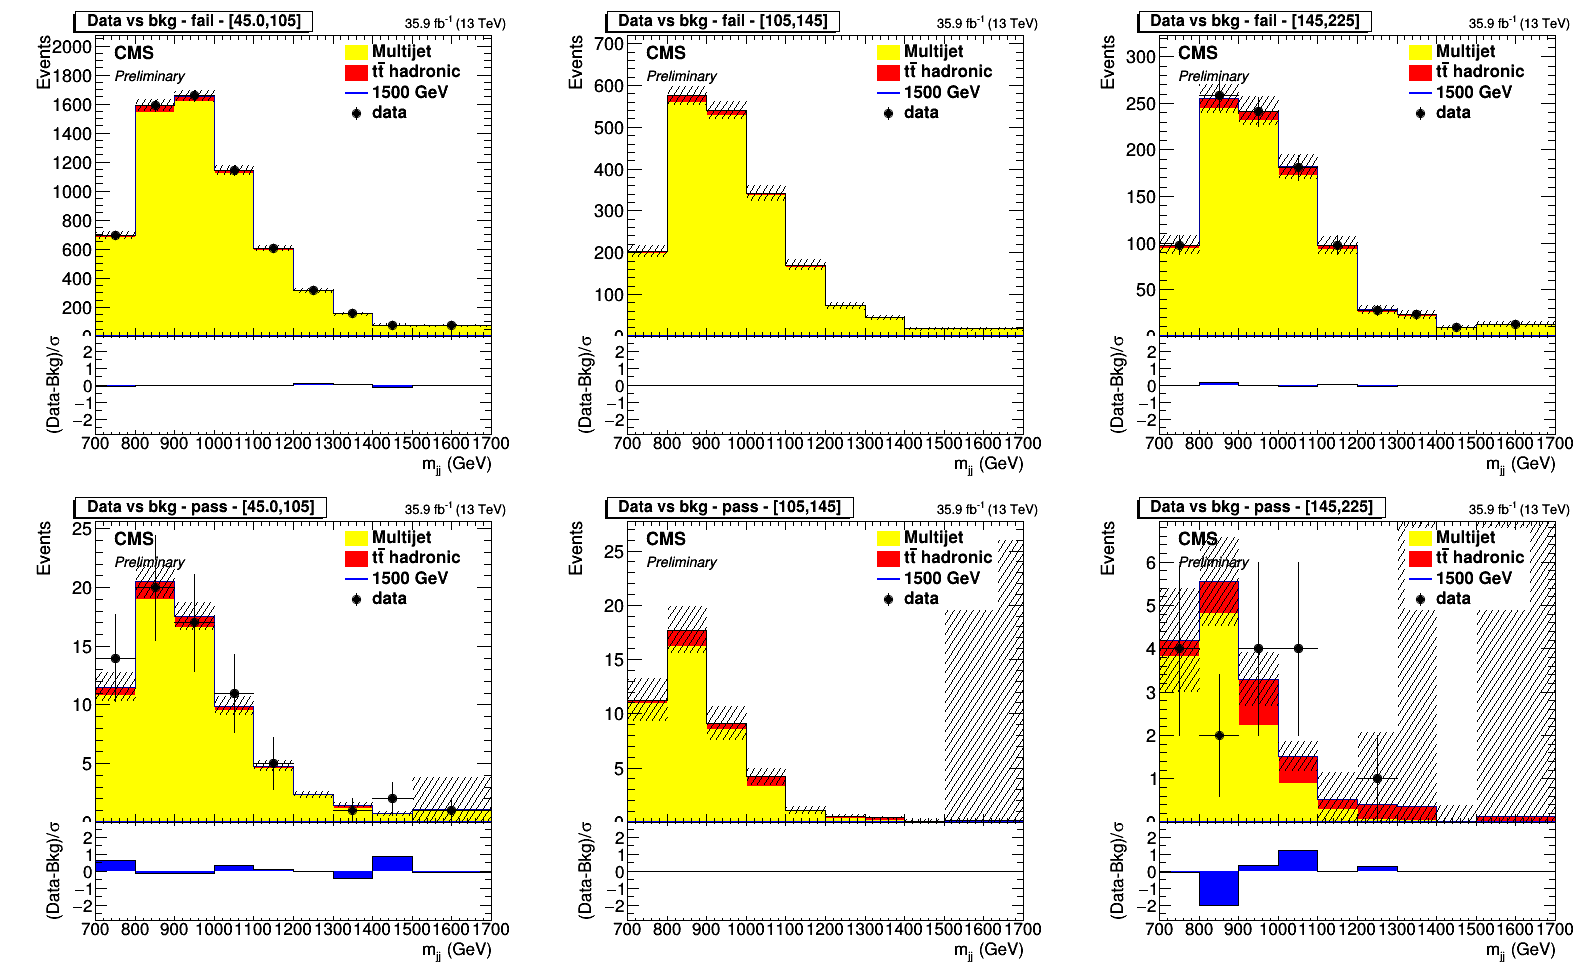
\includegraphics[width=1\textwidth]{Figures/postfit_projy_fits_1621.png}
	\caption{2016 2$+$1 background fits for $M_j$ axis and $M_{jj}^{red}$ axis including expected Radion 1500 GeV signal, normalized to the signal strength found by the fit.}
	\label{fig:1621}
\end{figure}
\begin{figure}[!htb]
	\centering
	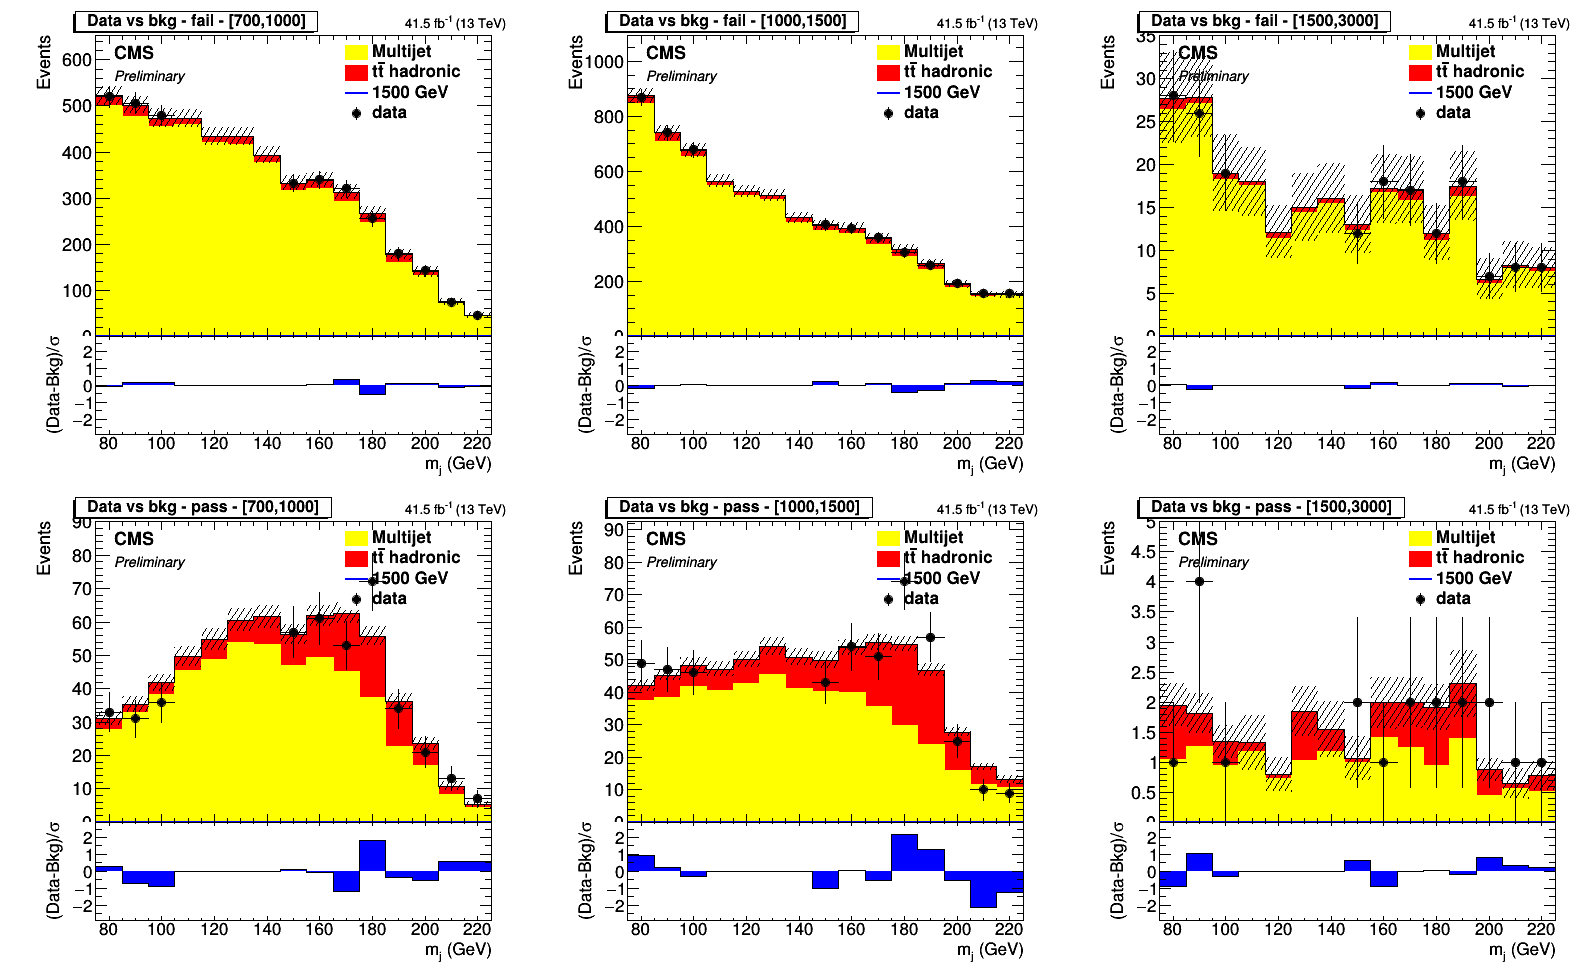
\includegraphics[width=1\textwidth]{Figures/postfit_projx_fits_17LL.png}
	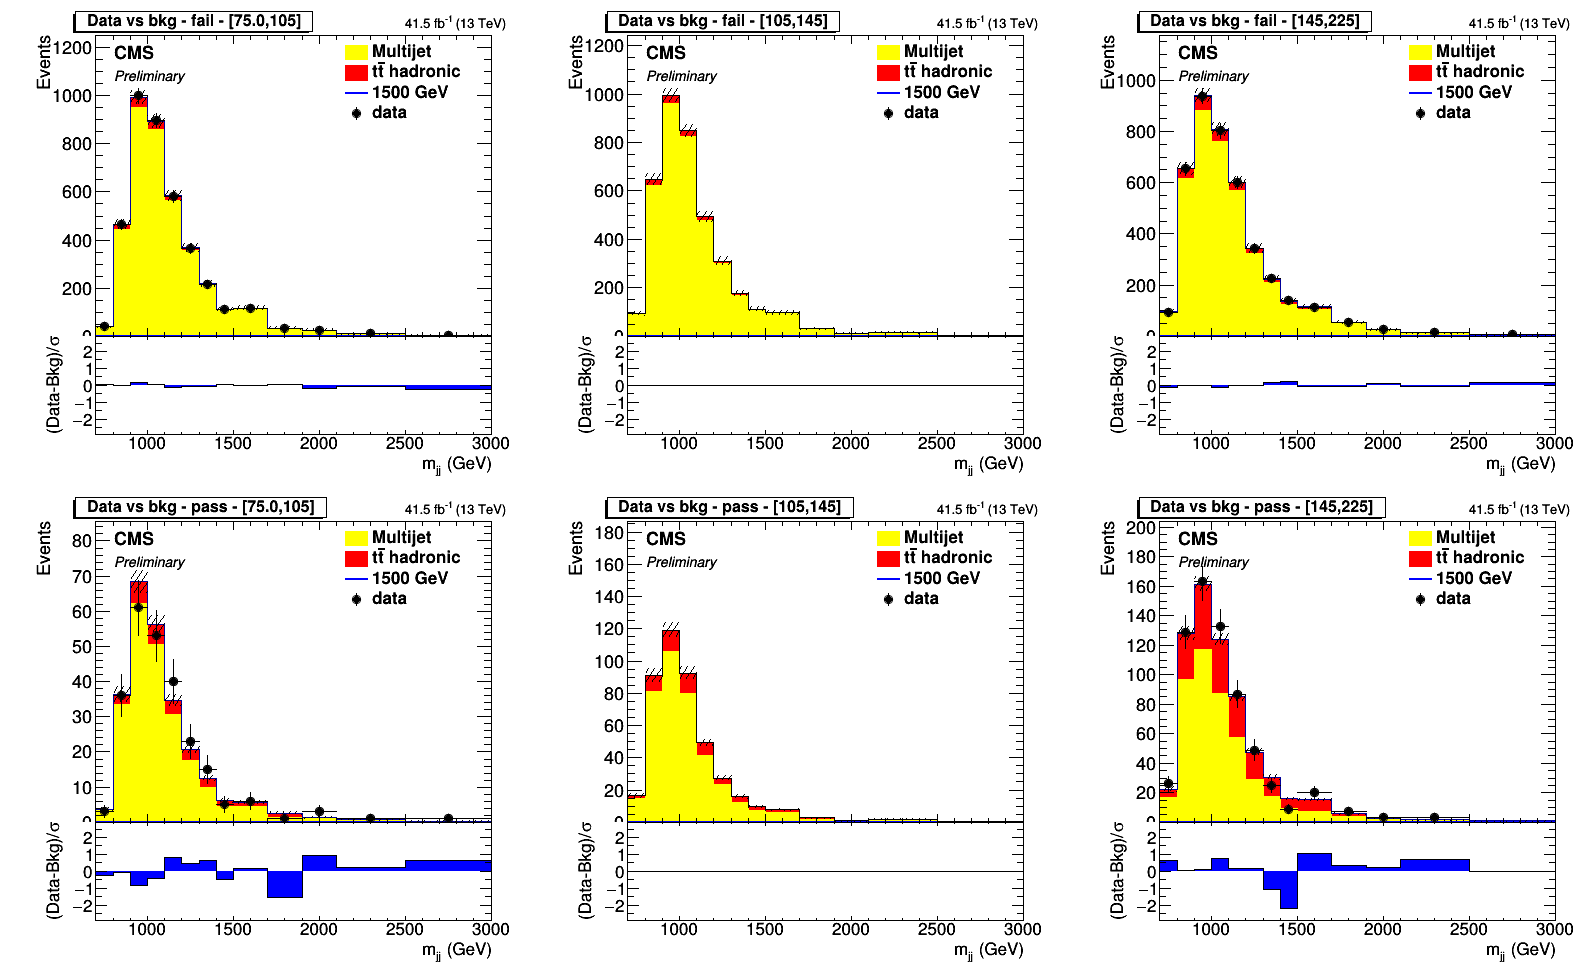
\includegraphics[width=1\textwidth]{Figures/postfit_projy_fits_17LL.png}
	\caption{2017 Loose Loose background fits for $M_j$ axis and $M_{jj}^{red}$ axis including expected Radion 1500 GeV signal, normalized to the signal strength found by the fit.}
	\label{fig:17LL}
\end{figure}
\begin{figure}[!htb]
	\centering
	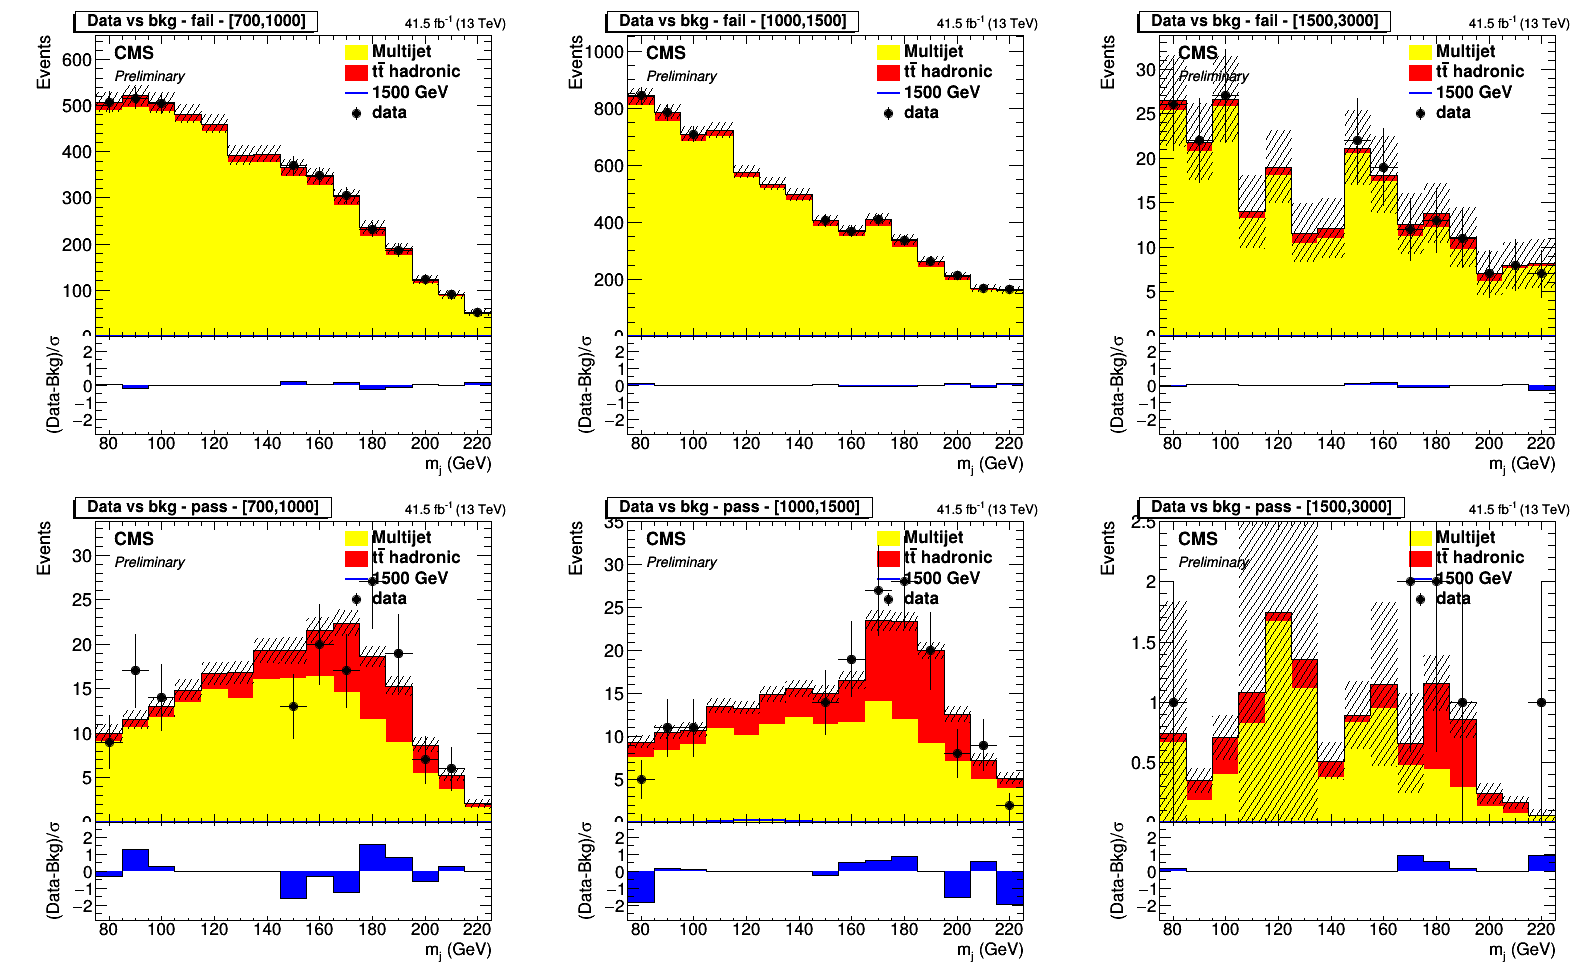
\includegraphics[width=\textwidth]{Figures/postfit_projx_fits_17TT.png}
	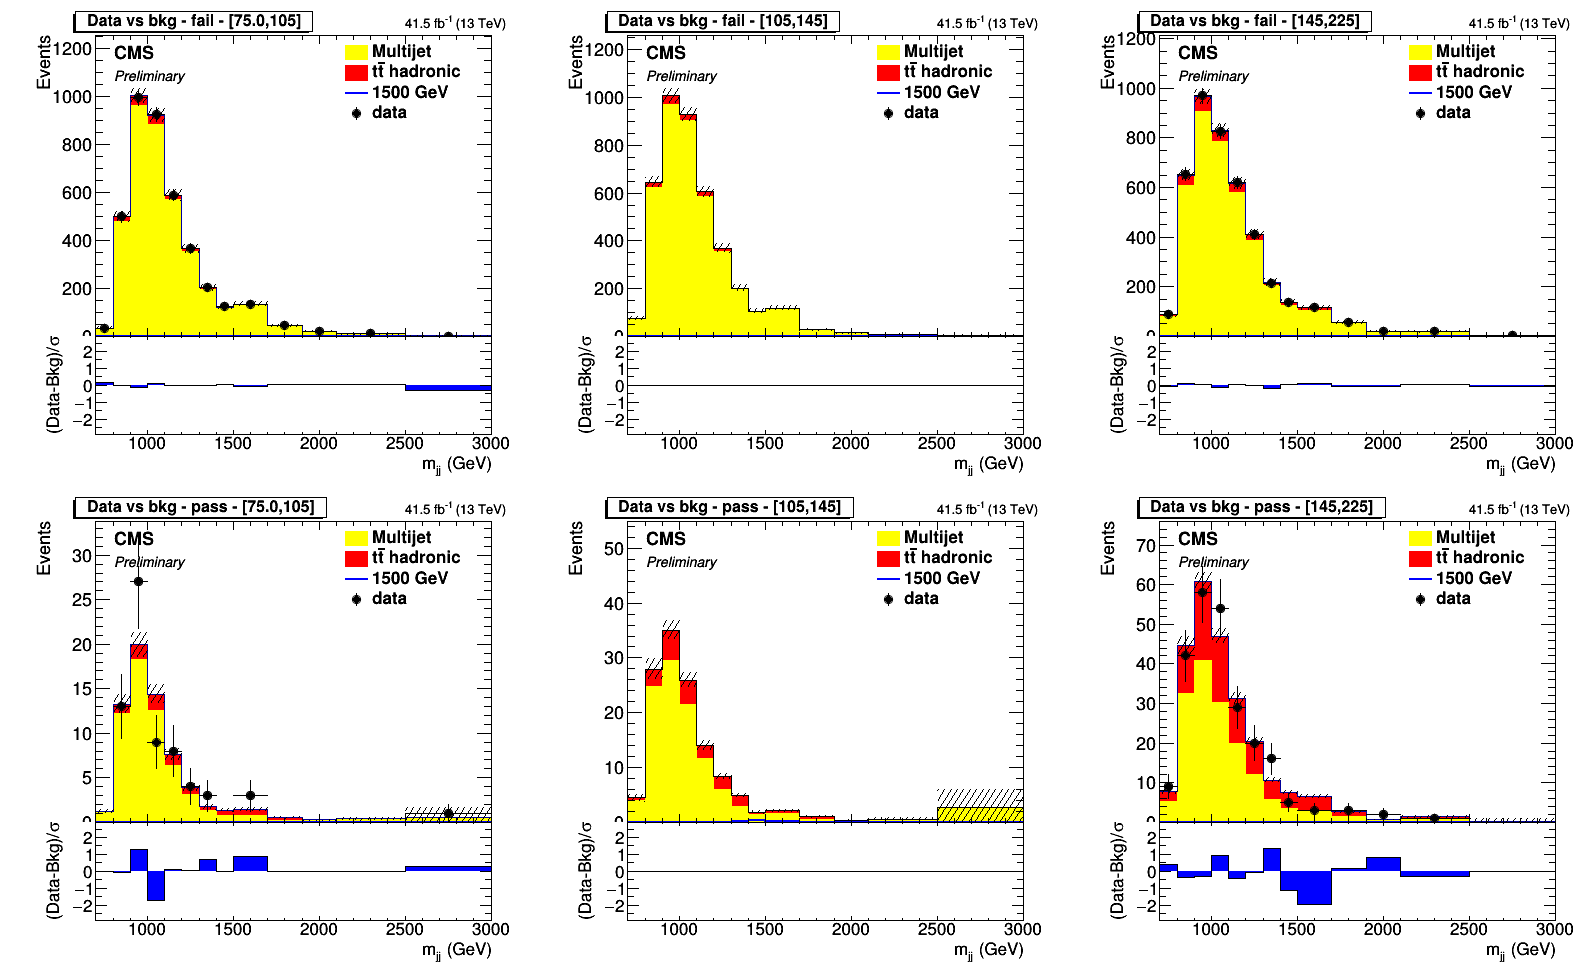
\includegraphics[width=1\textwidth]{Figures/postfit_projy_fits_17TT.png}
	\caption{2017 Tight Tight background fits for $M_j$ axis and $M_{jj}^{red}$ axis including expected Radion 1500 GeV signal, normalized to the signal strength found by the fit.}
	\label{fig:17TT}
\end{figure}
\begin{figure}[!htb]
	\centering
	\includegraphics[width=1\textwidth]{Figures/postfit_projx_fits_1721.png}
	\includegraphics[width=1\textwidth]{Figures/postfit_projy_fits_1721.png}
	\caption{2017 2$+$1 background fits for $M_j$ axis and $M_{jj}^{red}$ axis including expected Radion 1500 GeV signal, normalized to the signal strength found by the fit.}
	\label{fig:1721}
\end{figure}
\begin{figure}[!htb]
	\centering
	\includegraphics[width=1\textwidth]{Figures/postfit_projx_fits_18LL.png}
	\includegraphics[width=1\textwidth]{Figures/postfit_projy_fits_18LL.png}
	\caption{2018 Loose Loose background fits for $M_j$ axis and $M_{jj}^{red}$ axis including expected Radion 1500 GeV signal, normalized to the signal strength found by the fit.}
	\label{fig:18LL}
\end{figure}
\begin{figure}[!htb]
	\centering
	\includegraphics[width=1\textwidth]{Figures/postfit_projx_fits_18TT.png}
	\includegraphics[width=1\textwidth]{Figures/postfit_projy_fits_18TT.png}
	\caption{2018 Tight Tight background fits for $M_j$ axis and $M_{jj}^{red}$ axis including expected Radion 1500 GeV signal, normalized to the signal strength found by the fit.}
	\label{fig:18TT}
\end{figure}
\begin{figure}[!htb]
	\centering
	\includegraphics[width=1\textwidth]{Figures/postfit_projx_fits_1821.png}
	\includegraphics[width=1\textwidth]{Figures/postfit_projy_fits_1821.png}
	\caption{2018 2$+$1 background fits for $M_j$ axis and $M_{jj}^{red}$ axis including expected Radion 1500 GeV signal, normalized to the signal strength found by the fit.}
	\label{fig:1821}
\end{figure}
\begin{figure}[!htb]
	\centering
	\includegraphics[width=0.75\textwidth]{Figures/nuisance_pulls_byYear.pdf}
	\caption{Full Run 2 Nuissance Pulls Plot.}
	\label{fig:nuissancesAppend}
\end{figure}
\begin{figure}[!htb]
	\centering
	\includegraphics[width=0.75\textwidth]{Figures/impacts_byYear.pdf}
	\caption{Full Run 2 Impacts plot.}
	\label{fig:ImpactsplotAppend}
\end{figure}
\begin{figure}[!htb]
	\centering
	\includegraphics[width=1\textwidth]{Figures/postfit_projy_fits_log_16LL.png}
	\caption{2016 Loose Loose background fit for $M_{jj}^{red}$ log-scale axis including expected Radion 1500 GeV signal, normalized to the signal strength found by the fit.}
	\label{fig:16LLlog}
\end{figure}
\begin{figure}[!htb]
	\centering
	\includegraphics[width=1\textwidth]{Figures/postfit_projy_fits_log_16TT.png}
	\caption{2016 Tight Tight background fits for $M_{jj}^{red}$ log-scale axis including expected Radion 1500 GeV signal, normalized to the signal strength found by the fit.}
	\label{fig:16TTlog}
\end{figure}
\begin{figure}[!htb]
	\centering
	\includegraphics[width=1\textwidth]{Figures/postfit_projy_fits_log_17LL.png}
	\caption{2017 Loose Loose background fits for $M_{jj}^{red}$ log-scale axis including expected Radion 1500 GeV signal, normalized to the signal strength found by the fit.}
	\label{fig:17LLlog}
\end{figure}
\begin{figure}[!htb]
	\centering
	\includegraphics[width=1\textwidth]{Figures/postfit_projy_fits_log_17TT.png}
	\caption{2017 Tight Tight background fits for $M_{jj}^{red}$ log-scale axis including expected Radion 1500 GeV signal, normalized to the signal strength found by the fit.}
	\label{fig:17TTlog}
\end{figure}
\begin{figure}[!htb]
	\centering
	\includegraphics[width=1\textwidth]{Figures/postfit_projy_fits_log_18LL.png}
	\caption{2018 Loose Loose background fits for $M_{jj}^{red}$ log-scale axis including expected Radion 1500 GeV signal, normalized to the signal strength found by the fit.}
	\label{fig:18LLlog}
\end{figure}
\begin{figure}[!htb]
	\centering
	\includegraphics[width=1\textwidth]{Figures/postfit_projy_fits_log_18TT.png}
	\caption{2018 Tight Tight background fits for $M_{jj}^{red}$ log-scale axis including expected Radion 1500 GeV signal, normalized to the signal strength found by the fit.}
	\label{fig:18TTlog}
\end{figure}
\clearpage
\subsection{MC distributions before applying Selections\label{ss:beforeDistbyYear}}
The kinematic variables before the application of H->bb tagger(s), are shown in Figs.\ref{fig:prePtlead} through \ref{fig:preMred}. Here, the distributions are normalized to luminosity and the signal is normalized to 50\%. Also, the difference between TT and LL distributions is in the weight used for each. Since the deepTagMD$\_$HbbvsQCD tagger has not been applied yet, these differences may be small and not show up in these plots.
\begin{figure}[!htb]
	\centering
	\includegraphics[width=0.4\textwidth]{Figures/pt0LL_16_deepTagMD_HbbvsQCD.png}
	\includegraphics[width=0.4\textwidth]{Figures/pt0LL_17_deepTagMD_HbbvsQCD.png}
	\includegraphics[width=0.4\textwidth]{Figures/pt0LL_18_deepTagMD_HbbvsQCD.png}
	\includegraphics[width=0.4\textwidth]{Figures/pt0TT_16_deepTagMD_HbbvsQCD.png}
	\includegraphics[width=0.4\textwidth]{Figures/pt0TT_17_deepTagMD_HbbvsQCD.png}
	\includegraphics[width=0.4\textwidth]{Figures/pt0TT_18_deepTagMD_HbbvsQCD.png}
	\caption{Pre deepTagMD$\_$HbbvsQCD selection $p_T$ distribution of leading jet}
	\label{fig:prePtleadBY}
\end{figure}
\begin{figure}[!htb]
	\centering
	\includegraphics[width=0.4\textwidth]{Figures/pt1LL_16_deepTagMD_HbbvsQCD.png}
	\includegraphics[width=0.4\textwidth]{Figures/pt1LL_17_deepTagMD_HbbvsQCD.png}
	\includegraphics[width=0.4\textwidth]{Figures/pt1LL_18_deepTagMD_HbbvsQCD.png}
	\includegraphics[width=0.4\textwidth]{Figures/pt1TT_16_deepTagMD_HbbvsQCD.png}
	\includegraphics[width=0.4\textwidth]{Figures/pt1TT_17_deepTagMD_HbbvsQCD.png}
	\includegraphics[width=0.4\textwidth]{Figures/pt1TT_18_deepTagMD_HbbvsQCD.png}
	\caption{Pre deepTagMD$\_$HbbvsQCD selection $p_T$ distribution of subleading jet}
	\label{fig:prePtsubBY}
\end{figure}
\begin{figure}[!htb]
	\centering
	\includegraphics[width=0.4\textwidth]{Figures/eta0LL_16_deepTagMD_HbbvsQCD.png}
	\includegraphics[width=0.4\textwidth]{Figures/eta0LL_17_deepTagMD_HbbvsQCD.png}
	\includegraphics[width=0.4\textwidth]{Figures/eta0LL_18_deepTagMD_HbbvsQCD.png}
	\includegraphics[width=0.4\textwidth]{Figures/eta0TT_16_deepTagMD_HbbvsQCD.png}
	\includegraphics[width=0.4\textwidth]{Figures/eta0TT_17_deepTagMD_HbbvsQCD.png}
	\includegraphics[width=0.4\textwidth]{Figures/eta0TT_18_deepTagMD_HbbvsQCD.png}
	\caption{Pre deepTagMD$\_$HbbvsQCD selection $\eta$ distribution of leading jet}
	\label{fig:preEtaleadBY}
\end{figure}
\begin{figure}[!htb]
	\centering
	\includegraphics[width=0.4\textwidth]{Figures/eta1LL_16_deepTagMD_HbbvsQCD.png}
	\includegraphics[width=0.4\textwidth]{Figures/eta1LL_17_deepTagMD_HbbvsQCD.png}
	\includegraphics[width=0.4\textwidth]{Figures/eta1LL_18_deepTagMD_HbbvsQCD.png}
	\includegraphics[width=0.4\textwidth]{Figures/eta1TT_16_deepTagMD_HbbvsQCD.png}
	\includegraphics[width=0.4\textwidth]{Figures/eta1TT_17_deepTagMD_HbbvsQCD.png}
	\includegraphics[width=0.4\textwidth]{Figures/eta1TT_18_deepTagMD_HbbvsQCD.png}
	\caption{Pre deepTagMD$\_$HbbvsQCD selection $\eta$ distribution of subleading jet}
	\label{fig:preEtasubBY}
\end{figure}
\begin{figure}[!htb]
	\centering
	\includegraphics[width=0.4\textwidth]{Figures/deltaEtaLL_16_deepTagMD_HbbvsQCD.png}
	\includegraphics[width=0.4\textwidth]{Figures/deltaEtaLL_17_deepTagMD_HbbvsQCD.png}
	\includegraphics[width=0.4\textwidth]{Figures/deltaEtaLL_18_deepTagMD_HbbvsQCD.png}
	\includegraphics[width=0.4\textwidth]{Figures/deltaEtaTT_16_deepTagMD_HbbvsQCD.png}
	\includegraphics[width=0.4\textwidth]{Figures/deltaEtaTT_17_deepTagMD_HbbvsQCD.png}
	\includegraphics[width=0.4\textwidth]{Figures/deltaEtaTT_18_deepTagMD_HbbvsQCD.png}
	\caption{Pre deepTagMD$\_$HbbvsQCD selection $\Delta \eta$ distribution}
	\label{fig:predeltaEtaBY}
\end{figure}
\begin{figure}[!htb]
	\centering
	\includegraphics[width=0.4\textwidth]{Figures/msd0LL_16_deepTagMD_HbbvsQCD.png}
	\includegraphics[width=0.4\textwidth]{Figures/msd0LL_17_deepTagMD_HbbvsQCD.png}
	\includegraphics[width=0.4\textwidth]{Figures/msd0LL_18_deepTagMD_HbbvsQCD.png}
	\includegraphics[width=0.4\textwidth]{Figures/msd0TT_16_deepTagMD_HbbvsQCD.png}
	\includegraphics[width=0.4\textwidth]{Figures/msd0TT_17_deepTagMD_HbbvsQCD.png}
	\includegraphics[width=0.4\textwidth]{Figures/msd0TT_18_deepTagMD_HbbvsQCD.png}
	\caption{Pre deepTagMD$\_$HbbvsQCD selection $m_{j}$ distribution}
	\label{fig:premsd0BY}
\end{figure}
\begin{figure}[!htb]
	\centering
	\includegraphics[width=0.4\textwidth]{Figures/mredLL_16_deepTagMD_HbbvsQCD.png}
	\includegraphics[width=0.4\textwidth]{Figures/mredLL_17_deepTagMD_HbbvsQCD.png}
	\includegraphics[width=0.4\textwidth]{Figures/mredLL_18_deepTagMD_HbbvsQCD.png}
	\includegraphics[width=0.4\textwidth]{Figures/mredTT_16_deepTagMD_HbbvsQCD.png}
	\includegraphics[width=0.4\textwidth]{Figures/mredTT_17_deepTagMD_HbbvsQCD.png}
	\includegraphics[width=0.4\textwidth]{Figures/mredTT_18_deepTagMD_HbbvsQCD.png}
	\caption{Pre deepTagMD$\_$HbbvsQCD selection $m_{jj}$ distribution}
	\label{fig:preMredBY}
\end{figure}
\clearpage
\section{Limits by Year}
\begin{figure}[!htb]
	\centering
	\includegraphics[width=0.4\textwidth]{Figures/limits_combine_35_9fb_dak8MDHbb_signals16_RadNar.png}
	\includegraphics[width=0.4\textwidth]{Figures/limits_combine_45_5fb_dak8MDHbb_signals17_RadNar.png}
	\includegraphics[width=0.4\textwidth]{Figures/limits_combine_59_6fb_dak8MDHbb_signals18_RadNar.png}
	\caption{2016,2017,2018 Radion Limits for 1+1 and 2+1 using the Deep AK8 Mass Decorrelated Hbb Tagger.}
	\label{fig:RadionLimit161718}
\end{figure}

\begin{figure}[!htb]
	\centering
	\includegraphics[width=0.4\textwidth]{Figures/limits_combine_35_9fb_dak8MDHbb_signals16_GravNar.png}
	\includegraphics[width=0.4\textwidth]{Figures/limits_combine_45_5fb_dak8MDHbb_signals17_GravNar.png}
	\includegraphics[width=0.4\textwidth]{Figures/limits_combine_59_6fb_dak8MDHbb_signals18_GravNar.png}
	\caption{2016,2017,2018 Graviton Limits for 1+1 and 2+1 using the Deep AK8 Mass Decorrelated Hbb Tagger.}
	\label{fig:GravitonLimit161718}
\end{figure}
\clearpage
\section{Deep AK8 MD Hbb Tagger Working Point Study}
The following study was conducted to optimize the working points for the boosted and semi-resolved analysis since official working points are not available for this tagger. We scan the deepAK8 score and find that we should choose a working point as close to $1$ as possible without totally eliminating the background in order to do a background estimate. 
We originally chose 0.95 for the TT working point but ended up relaxing it to 0.9 because of the extreme nature of the cut. Here we present just the 1500 GeV mass point for Narrow Radion and Bulk Graviton but the other mass points have the same conclusion. We also do the same study with just \ttbar as a background to make sure the same conclusion is reached, which it is.
\begin{figure}[!htb]
	\centering
	\includegraphics[width=0.5\textwidth]{Figures/wp_RadNar1500.png}
	\includegraphics[width=0.5\textwidth]{Figures/wp_GravNar1500.png}
	\caption{Optimization of dak8MDHbb tagger using $S/\sqrt{B}$ for Narrow Radion and Bulk Graviton 1500 Gev.}
	\label{fig:SoversqrtBstudy}
\end{figure}
\begin{figure}[!htb]
	\centering
	\includegraphics[width=0.5\textwidth]{Figures/wp_RadNar1500_ttbar.png}
	\includegraphics[width=0.5\textwidth]{Figures/wp_GravNar1500_ttbar.png}
	\caption{Optimization of dak8MDHbb tagger using $S/\sqrt{B}$ for Narrow Radion and Bulk Graviton 1500 Gev with just \ttbar as a background.}
	\label{fig:SoversqrtBstudyttbar}
\end{figure}
\clearpage
\section{Trigger Scale Factor}
In previous version of this analysis, the trigger efficiency in data was used to correct the trigger response in MC. The latest method is documented in \ref{s:trigger}. Here we show the comparison of the two methods.
\begin{figure}[!htb]
	\centering
	\includegraphics[width=0.5\textwidth]{Figures/triggerMethodComparisonstudy2016.png}
	\caption{Comparison of trigger scale factors for 2016.}
	\label{fig:triggerStudy16}
\end{figure}
\begin{figure}[!htb]
	\centering
	\includegraphics[width=0.5\textwidth]{Figures/triggerMethodComparisonstudy2017.png}
	\caption{Comparison of trigger scale factors for 2017.}
	\label{fig:triggerStudy17}
\end{figure}
\begin{figure}[!htb]
	\centering
	\includegraphics[width=0.5\textwidth]{Figures/triggerMethodComparisonstudy2018.png}
	\caption{Comparison of trigger scale factors for 2018.}
	\label{fig:triggerStudy18}
\end{figure}
\clearpage
\section{Jet Energy Resolution Template Examples\label{s:jerExamples}}
Here we show example Jet Energy and Mass correction templates of both resolution and scale for Radion at 1500 GeV and $\ttbar$, for the year 2016 and the TT region as an example. 
\begin{figure}[!htb]
	\centering
	\includegraphics[width=0.4\textwidth]{Figures/Uncertainty_16_RadNar-1500_jer16failX.png}
	\includegraphics[width=0.4\textwidth]{Figures/Uncertainty_16_RadNar-1500_jer16passX.png}
	\includegraphics[width=0.4\textwidth]{Figures/Uncertainty_16_RadNar-1500_jer16failY.png}
	\includegraphics[width=0.4\textwidth]{Figures/Uncertainty_16_RadNar-1500_jer16passY.png}
	\caption{2016 Narrow Radion 1500 GeV JER pass and fail templates for $M_j$ axis and $M_{jj}^{red}$ axis.}
	\label{fig:jerRadion1}
\end{figure}
\begin{figure}[!htb]
	\centering
	\includegraphics[width=0.4\textwidth]{Figures/Uncertainty_16_ttbar_smoothed_1_2_jer16failX.png}
	\includegraphics[width=0.4\textwidth]{Figures/Uncertainty_16_ttbar_smoothed_1_2_jer16passX.png}
	\includegraphics[width=0.4\textwidth]{Figures/Uncertainty_16_ttbar_smoothed_1_2_jer16failY.png}
	\includegraphics[width=0.4\textwidth]{Figures/Uncertainty_16_ttbar_smoothed_1_2_jer16passY.png}
	\caption{2016 $\ttbar$ JER pass and fail templates for $M_j$ axis and $M_{jj}^{red}$ axis.}
	\label{fig:jerttbar1}
\end{figure}

\begin{figure}[!htb]
	\centering
	\includegraphics[width=0.4\textwidth]{Figures/Uncertainty_16_RadNar-1500_jes16failX.png}
	\includegraphics[width=0.4\textwidth]{Figures/Uncertainty_16_RadNar-1500_jes16passX.png}
	\includegraphics[width=0.4\textwidth]{Figures/Uncertainty_16_RadNar-1500_jes16failY.png}
	\includegraphics[width=0.4\textwidth]{Figures/Uncertainty_16_RadNar-1500_jes16passY.png}
	\caption{2016 Narrow Radion 1500 GeV JES pass and fail templates for $M_j$ axis and $M_{jj}^{red}$ axis.}
	\label{fig:jesRadion2}
\end{figure}
\begin{figure}[!htb]
	\centering
	\includegraphics[width=0.4\textwidth]{Figures/Uncertainty_16_ttbar_smoothed_1_2_jes16failX.png}
	\includegraphics[width=0.4\textwidth]{Figures/Uncertainty_16_ttbar_smoothed_1_2_jes16passX.png}
	\includegraphics[width=0.4\textwidth]{Figures/Uncertainty_16_ttbar_smoothed_1_2_jes16failY.png}
	\includegraphics[width=0.4\textwidth]{Figures/Uncertainty_16_ttbar_smoothed_1_2_jes16passY.png}
	\caption{2016 $\ttbar$ JES pass and fail templates for $M_j$ axis and $M_{jj}^{red}$ axis.}
	\label{fig:jesttbar2}
\end{figure}

\begin{figure}[!htb]
	\centering
	\includegraphics[width=0.4\textwidth]{Figures/Uncertainty_16_RadNar-1500_jmr16failX.png}
	\includegraphics[width=0.4\textwidth]{Figures/Uncertainty_16_RadNar-1500_jmr16passX.png}
	\includegraphics[width=0.4\textwidth]{Figures/Uncertainty_16_RadNar-1500_jmr16failY.png}
	\includegraphics[width=0.4\textwidth]{Figures/Uncertainty_16_RadNar-1500_jmr16passY.png}
	\caption{2016 Narrow Radion 1500 GeV JMR pass and fail templates for $M_j$ axis and $M_{jj}^{red}$ axis.}
	\label{fig:jerRadionAppend}
\end{figure}
\begin{figure}[!htb]
	\centering
	\includegraphics[width=0.4\textwidth]{Figures/Uncertainty_16_ttbar_smoothed_1_2_jmr16failX.png}
	\includegraphics[width=0.4\textwidth]{Figures/Uncertainty_16_ttbar_smoothed_1_2_jmr16passX.png}
	\includegraphics[width=0.4\textwidth]{Figures/Uncertainty_16_ttbar_smoothed_1_2_jmr16failY.png}
	\includegraphics[width=0.4\textwidth]{Figures/Uncertainty_16_ttbar_smoothed_1_2_jmr16passY.png}
	\caption{2016 $\ttbar$ JMR pass and fail templates for $M_j$ axis and $M_{jj}^{red}$ axis.}
	\label{fig:jerttbarAppend}
\end{figure}

\begin{figure}[!htb]
	\centering
	\includegraphics[width=0.4\textwidth]{Figures/Uncertainty_16_RadNar-1500_jms16failX.png}
	\includegraphics[width=0.4\textwidth]{Figures/Uncertainty_16_RadNar-1500_jms16passX.png}
	\includegraphics[width=0.4\textwidth]{Figures/Uncertainty_16_RadNar-1500_jms16failY.png}
	\includegraphics[width=0.4\textwidth]{Figures/Uncertainty_16_RadNar-1500_jms16passY.png}
	\caption{2016 Narrow Radion 1500 GeV JMS pass and fail templates for $M_j$ axis and $M_{jj}^{red}$ axis.}
	\label{fig:jesRadionAppend}
\end{figure}
\begin{figure}[!htb]
	\centering
	\includegraphics[width=0.4\textwidth]{Figures/Uncertainty_16_ttbar_smoothed_1_2_jms16failX.png}
	\includegraphics[width=0.4\textwidth]{Figures/Uncertainty_16_ttbar_smoothed_1_2_jms16passX.png}
	\includegraphics[width=0.4\textwidth]{Figures/Uncertainty_16_ttbar_smoothed_1_2_jms16failY.png}
	\includegraphics[width=0.4\textwidth]{Figures/Uncertainty_16_ttbar_smoothed_1_2_jms16passY.png}
	\caption{2016 $\ttbar$ JMS pass and fail templates for $M_j$ axis and $M_{jj}^{red}$ axis.}
	\label{fig:jesttbarAppend}
\end{figure}
\clearpage
\section{$\mred$ Dependent $\Delta \eta_{jj}$ Cut studies\label{s:mredDeltaEta}}
We studied the effect on both the signal efficiency and the limits of introducing a $\mred$ dependent $\Delta \eta_{jj}$ cut in order to try to capture any lost signal, particularly at higher resonance masses.
We concluded that although the signal efficiency for each region and resonance mass point increases, it does not do so enough to make a difference in the expected limits and therefore we do not implement this change.
\begin{figure}[!htb]
	\centering
	\includegraphics[width=0.5\textwidth]{Figures/sigEffrad_combined_Run2_deepTagMD_HbbvsQCD_base.png}
	\caption{Radion Signal Efficiency for full Run 2.}
	\label{fig:sigEffRad}
\end{figure}
\begin{figure}[!htb]
	\centering
	\includegraphics[width=0.5\textwidth]{Figures/sigEffgrav_combined_Run2_deepTagMD_HbbvsQCD_base.png}
	\caption{Radion Signal Efficiency for full Run 2.}
	\label{fig:sigEffGrav}
\end{figure}

\begin{figure}[!htb]
	\centering
	\includegraphics[width=0.5\textwidth]{Figures/sigEffrad_combined_Run2_deepTagMD_HbbvsQCD_mred.png}
	\caption{Radion Signal Efficiency for full Run 2 with $\mred$ Dependent $\Delta \eta_{jj}$ Cut.}
	\label{fig:sigEffRadmred}
\end{figure}
\begin{figure}[!htb]
	\centering
	\includegraphics[width=0.5\textwidth]{Figures/sigEffgrav_combined_Run2_deepTagMD_HbbvsQCD_mred.png}
	\caption{Radion Signal Efficiency for full Run 2 with $\mred$ Dependent $\Delta \eta_{jj}$ Cut.}
	\label{fig:sigEffGravmred}
\end{figure}
\begin{figure}[!htb]
	\centering
	\includegraphics[width=0.5\textwidth]{Figures/limits_HH_combine_137fb_deltaEtaComparison_RadNar_fixedmredDeltaEtaCheckRadion.pdf}
	\caption{Full Run 2 Radion Limit comparison with $\mred$ Dependent $\Delta \eta_{jj}$ Cut.}
	\label{fig:RadionLimitFULLmred}
\end{figure}

\begin{figure}[!htb]
	\centering
	\includegraphics[width=0.5\textwidth]{Figures/limits_HH_combine_137fb_deltaEtaComparison_GravNar_fixedmredDeltaEtaCheckGraviton.pdf}
	\caption{Full Run 2 Graviton Limit comparison with $\mred$ Dependent $\Delta \eta_{jj}$ Cut.}
	\label{fig:GravitonLimitFULLmred}
\end{figure}
\clearpage
\section{Wide Resonances}
We perform this analysis for resonances with a higher width as a check of the validity of the background estimate. Here we show both the unblinded results for the bulk graviton and radion signal samples with a 10\% width. 
\begin{figure}[!htb]
	\centering
	\includegraphics[width=1\textwidth]{Figures/postfit_projx_fits_LLwide.pdf}
	\caption{Full Run 2 Loose Loose fits for $M_j$ axis including expected Radion 2000 GeV wide signal, normalized to the signal strength found by the fit.}
	\label{fig:LLmjwide}
\end{figure}
\begin{figure}[!htb]
	\centering
	\includegraphics[width=1\textwidth]{Figures/postfit_projy_fits_LLwide.pdf}
	\caption{Full Run 2 Loose Loose fits for $M_{jj}^{red}$ axis including expected Radion 2000 GeV wide signal, normalized to the signal strength found by the fit.}
	\label{fig:LLmjjwide}
\end{figure}
\begin{figure}[!htb]
	\centering
	\includegraphics[width=1\textwidth]{Figures/postfit_projx_fits_TTwide.pdf}
	\caption{Full Run 2 Tight Tight fits for $M_j$ axis including expected Radion 2000 GeV wide signal, normalized to the signal strength found by the fit.}
	\label{fig:TTmjwide}
\end{figure}
\begin{figure}[!htb]
	\centering
	\includegraphics[width=1\textwidth]{Figures/postfit_projy_fits_TTwide.pdf}
	\caption{Full Run 2 Tight Tight fits for $M_{jj}^{red}$ axis including expected Radion 2000 GeV wide signal, normalized to the signal strength found by the fit.}
	\label{fig:TTmjjwide}
\end{figure}
\begin{figure}[!htb]
	\centering
	\includegraphics[width=1\textwidth]{Figures/postfit_projx_fits_21wide.pdf}
	\caption{Full Run 2 2$+$1 fits for $M_j$ axis including expected Radion 2000 GeV wide signal, normalized to the signal strength found by the fit.}
	\label{fig:21mjwide}
\end{figure}
\begin{figure}[!htb]
	\centering
	\includegraphics[width=1\textwidth]{Figures/postfit_projy_fits_21wide.pdf}
	\caption{Full Run 2 2$+$1 fits for $M_{jj}^{red}$ axis including expected Radion 2000 GeV wide signal, normalized to the signal strength found by the fit.}
	\label{fig:21mjjwide}
\end{figure}
\begin{figure}[!htb]
	\centering
	\includegraphics[width=1\textwidth]{Figures/nuisance_pulls_wide.pdf}
	\caption{Full Run 2 Nuissance Pulls Plot for 2 TeV wide Radion signal.}
	\label{fig:nuissanceswide}
\end{figure}

\begin{figure}[!htb]
	\centering
	\includegraphics[width=0.75\textwidth]{Figures/gof_plot_wide.pdf}
	\caption{Full Run 2 Goodness of Fit test plot with 500 toys for 2 TeV wide Radion signal.}
	\label{fig:gofplotwide}
\end{figure}
\begin{figure}[!htb]
	\centering
	\includegraphics[width=0.75\textwidth]{Figures/correlation_matrix_wide.png}
	\caption{Full Run 2 Correlation Matrix for 2 TeV wide Radion signal.}
	\label{fig:corrMatrixplotwide}
\end{figure}
\begin{figure}[!htb]
	\centering
	\includegraphics[width=0.4\textwidth]{Figures/signalInjection0_500_sigpull_1000wide.png}
	\includegraphics[width=0.4\textwidth]{Figures/signalInjection0_500_sigstrength_1000wide.png}
	\includegraphics[width=0.4\textwidth]{Figures/signalInjection1_500_sigpull_1000wide.png}
	\includegraphics[width=0.4\textwidth]{Figures/signalInjection1_500_sigstrength_1000wide.png}
	\includegraphics[width=0.4\textwidth]{Figures/signalInjection3_500_sigpull_1000wide.png}
	\includegraphics[width=0.4\textwidth]{Figures/signalInjection3_500_sigstrength_1000wide.png}
	\caption{Wide Signal (Left Column is Pull and Right is Strength) Injection for Full Run 2 at 1 TeV for r = 0, 1, 3 with 500 toys.}
	\label{fig:signalInjection1000plotwide}
\end{figure}

\begin{figure}[!htb]
	\centering
	\includegraphics[width=0.4\textwidth]{Figures/signalInjection0_500_sigpull_2000wide.png}
	\includegraphics[width=0.4\textwidth]{Figures/signalInjection0_500_sigstrength_2000wide.png}
	\includegraphics[width=0.4\textwidth]{Figures/signalInjection1_500_sigpull_2000wide.png}
	\includegraphics[width=0.4\textwidth]{Figures/signalInjection1_500_sigstrength_2000wide.png}
	\includegraphics[width=0.4\textwidth]{Figures/signalInjection3_500_sigpull_2000wide.png}
	\includegraphics[width=0.4\textwidth]{Figures/signalInjection3_500_sigstrength_2000wide.png}
	\caption{Wide Signal (Left Column is Pull and Right is Strength) Injection for Full Run 2 at 2 TeV for r = 0, 1, 3 with 500 toys.}
	\label{fig:signalInjection2000plotwide}
\end{figure}

\begin{figure}[!htb]
	\centering
	\includegraphics[width=0.4\textwidth]{Figures/signalInjection0_500_sigpull_3000wide.png}
	\includegraphics[width=0.4\textwidth]{Figures/signalInjection0_500_sigstrength_3000wide.png}
	\includegraphics[width=0.4\textwidth]{Figures/signalInjection1_500_sigpull_3000wide.png}
	\includegraphics[width=0.4\textwidth]{Figures/signalInjection1_500_sigstrength_3000wide.png}
	\includegraphics[width=0.4\textwidth]{Figures/signalInjection3_500_sigpull_3000wide.png}
	\includegraphics[width=0.4\textwidth]{Figures/signalInjection3_500_sigstrength_3000wide.png}
	\caption{Wide Signal (Left Column is Pull and Right is Strength) Injection for Full Run 2 at 3 TeV for r = 0, 1, 3 with 500 toys.}
	\label{fig:signalInjection3000plotwide}
\end{figure}